% Options for packages loaded elsewhere
\PassOptionsToPackage{unicode}{hyperref}
\PassOptionsToPackage{hyphens}{url}
%
\documentclass[
]{book}
\usepackage{lmodern}
\usepackage{amsmath}
\usepackage{ifxetex,ifluatex}
\ifnum 0\ifxetex 1\fi\ifluatex 1\fi=0 % if pdftex
  \usepackage[T1]{fontenc}
  \usepackage[utf8]{inputenc}
  \usepackage{textcomp} % provide euro and other symbols
  \usepackage{amssymb}
\else % if luatex or xetex
  \usepackage{unicode-math}
  \defaultfontfeatures{Scale=MatchLowercase}
  \defaultfontfeatures[\rmfamily]{Ligatures=TeX,Scale=1}
\fi
% Use upquote if available, for straight quotes in verbatim environments
\IfFileExists{upquote.sty}{\usepackage{upquote}}{}
\IfFileExists{microtype.sty}{% use microtype if available
  \usepackage[]{microtype}
  \UseMicrotypeSet[protrusion]{basicmath} % disable protrusion for tt fonts
}{}
\makeatletter
\@ifundefined{KOMAClassName}{% if non-KOMA class
  \IfFileExists{parskip.sty}{%
    \usepackage{parskip}
  }{% else
    \setlength{\parindent}{0pt}
    \setlength{\parskip}{6pt plus 2pt minus 1pt}}
}{% if KOMA class
  \KOMAoptions{parskip=half}}
\makeatother
\usepackage{xcolor}
\IfFileExists{xurl.sty}{\usepackage{xurl}}{} % add URL line breaks if available
\IfFileExists{bookmark.sty}{\usepackage{bookmark}}{\usepackage{hyperref}}
\hypersetup{
  pdftitle={Анализ данных для лингвистов},
  pdfauthor={Г. А. Мороз},
  hidelinks,
  pdfcreator={LaTeX via pandoc}}
\urlstyle{same} % disable monospaced font for URLs
\usepackage{color}
\usepackage{fancyvrb}
\newcommand{\VerbBar}{|}
\newcommand{\VERB}{\Verb[commandchars=\\\{\}]}
\DefineVerbatimEnvironment{Highlighting}{Verbatim}{commandchars=\\\{\}}
% Add ',fontsize=\small' for more characters per line
\usepackage{framed}
\definecolor{shadecolor}{RGB}{248,248,248}
\newenvironment{Shaded}{\begin{snugshade}}{\end{snugshade}}
\newcommand{\AlertTok}[1]{\textcolor[rgb]{0.94,0.16,0.16}{#1}}
\newcommand{\AnnotationTok}[1]{\textcolor[rgb]{0.56,0.35,0.01}{\textbf{\textit{#1}}}}
\newcommand{\AttributeTok}[1]{\textcolor[rgb]{0.77,0.63,0.00}{#1}}
\newcommand{\BaseNTok}[1]{\textcolor[rgb]{0.00,0.00,0.81}{#1}}
\newcommand{\BuiltInTok}[1]{#1}
\newcommand{\CharTok}[1]{\textcolor[rgb]{0.31,0.60,0.02}{#1}}
\newcommand{\CommentTok}[1]{\textcolor[rgb]{0.56,0.35,0.01}{\textit{#1}}}
\newcommand{\CommentVarTok}[1]{\textcolor[rgb]{0.56,0.35,0.01}{\textbf{\textit{#1}}}}
\newcommand{\ConstantTok}[1]{\textcolor[rgb]{0.00,0.00,0.00}{#1}}
\newcommand{\ControlFlowTok}[1]{\textcolor[rgb]{0.13,0.29,0.53}{\textbf{#1}}}
\newcommand{\DataTypeTok}[1]{\textcolor[rgb]{0.13,0.29,0.53}{#1}}
\newcommand{\DecValTok}[1]{\textcolor[rgb]{0.00,0.00,0.81}{#1}}
\newcommand{\DocumentationTok}[1]{\textcolor[rgb]{0.56,0.35,0.01}{\textbf{\textit{#1}}}}
\newcommand{\ErrorTok}[1]{\textcolor[rgb]{0.64,0.00,0.00}{\textbf{#1}}}
\newcommand{\ExtensionTok}[1]{#1}
\newcommand{\FloatTok}[1]{\textcolor[rgb]{0.00,0.00,0.81}{#1}}
\newcommand{\FunctionTok}[1]{\textcolor[rgb]{0.00,0.00,0.00}{#1}}
\newcommand{\ImportTok}[1]{#1}
\newcommand{\InformationTok}[1]{\textcolor[rgb]{0.56,0.35,0.01}{\textbf{\textit{#1}}}}
\newcommand{\KeywordTok}[1]{\textcolor[rgb]{0.13,0.29,0.53}{\textbf{#1}}}
\newcommand{\NormalTok}[1]{#1}
\newcommand{\OperatorTok}[1]{\textcolor[rgb]{0.81,0.36,0.00}{\textbf{#1}}}
\newcommand{\OtherTok}[1]{\textcolor[rgb]{0.56,0.35,0.01}{#1}}
\newcommand{\PreprocessorTok}[1]{\textcolor[rgb]{0.56,0.35,0.01}{\textit{#1}}}
\newcommand{\RegionMarkerTok}[1]{#1}
\newcommand{\SpecialCharTok}[1]{\textcolor[rgb]{0.00,0.00,0.00}{#1}}
\newcommand{\SpecialStringTok}[1]{\textcolor[rgb]{0.31,0.60,0.02}{#1}}
\newcommand{\StringTok}[1]{\textcolor[rgb]{0.31,0.60,0.02}{#1}}
\newcommand{\VariableTok}[1]{\textcolor[rgb]{0.00,0.00,0.00}{#1}}
\newcommand{\VerbatimStringTok}[1]{\textcolor[rgb]{0.31,0.60,0.02}{#1}}
\newcommand{\WarningTok}[1]{\textcolor[rgb]{0.56,0.35,0.01}{\textbf{\textit{#1}}}}
\usepackage{longtable,booktabs}
\usepackage{calc} % for calculating minipage widths
% Correct order of tables after \paragraph or \subparagraph
\usepackage{etoolbox}
\makeatletter
\patchcmd\longtable{\par}{\if@noskipsec\mbox{}\fi\par}{}{}
\makeatother
% Allow footnotes in longtable head/foot
\IfFileExists{footnotehyper.sty}{\usepackage{footnotehyper}}{\usepackage{footnote}}
\makesavenoteenv{longtable}
\usepackage{graphicx}
\makeatletter
\def\maxwidth{\ifdim\Gin@nat@width>\linewidth\linewidth\else\Gin@nat@width\fi}
\def\maxheight{\ifdim\Gin@nat@height>\textheight\textheight\else\Gin@nat@height\fi}
\makeatother
% Scale images if necessary, so that they will not overflow the page
% margins by default, and it is still possible to overwrite the defaults
% using explicit options in \includegraphics[width, height, ...]{}
\setkeys{Gin}{width=\maxwidth,height=\maxheight,keepaspectratio}
% Set default figure placement to htbp
\makeatletter
\def\fps@figure{htbp}
\makeatother
\setlength{\emergencystretch}{3em} % prevent overfull lines
\providecommand{\tightlist}{%
  \setlength{\itemsep}{0pt}\setlength{\parskip}{0pt}}
\setcounter{secnumdepth}{5}
\usepackage{booktabs}
\usepackage[utf8]{inputenc}
\usepackage[english,russian]{babel}
\usepackage{fontspec}
\setmainfont[Ligatures=TeX,
             Path=font/,
             BoldFont=brillb,
             ItalicFont=brilli,
             BoldItalicFont=brillbi]{brill}
\setmonofont[Scale=0.7,
             Path=font/]{iosevka-regular}

\usepackage{longtable}
\usepackage[bf,singlelinecheck=off]{caption}

\usepackage{framed,color}
\definecolor{shadecolor}{RGB}{248,248,248}

\renewcommand{\textfraction}{0.05}
\renewcommand{\topfraction}{0.8}
\renewcommand{\bottomfraction}{0.8}
\renewcommand{\floatpagefraction}{0.75}

\let\oldhref\href
\renewcommand{\href}[2]{#2\footnote{\url{#1}}}
  \makeatletter
  \newenvironment{kframe}{%
    \medskip{}
    \setlength{\fboxsep}{.8em}
    \def\at@end@of@kframe{}%
    \ifinner\ifhmode%
    \def\at@end@of@kframe{\end{minipage}}%
    \begin{minipage}{\columnwidth}%
    \fi\fi%
    \def\FrameCommand##1{\hskip\@totalleftmargin \hskip-\fboxsep
    \colorbox{shadecolor}{##1}\hskip-\fboxsep
      % There is no \\@totalrightmargin, so:
        \hskip-\linewidth \hskip-\@totalleftmargin \hskip\columnwidth}%
    \MakeFramed {\advance\hsize-\width
      \@totalleftmargin\z@ \linewidth\hsize
      \@setminipage}}%
  {\par\unskip\endMakeFramed%
    \at@end@of@kframe}
  \makeatother
  
  \makeatletter
  \@ifundefined{Shaded}{
  }{\renewenvironment{Shaded}{\begin{kframe}}{\end{kframe}}}
  \makeatother
  
  \newenvironment{rmdblock}[1]
  {
    \begin{itemize}
    \renewcommand{\labelitemi}{
      \raisebox{-.7\height}[0pt][0pt]{
        {\setkeys{Gin}{width=3em,keepaspectratio}\includegraphics{images/#1}}
        }
        }
        \setlength{\fboxsep}{1em}
        \begin{kframe}
        \item
      }
      {
        \end{kframe}
        \end{itemize}
      }
      \newenvironment{rmdtask}
      {\begin{rmdblock}{task}}
      {\end{rmdblock}}
      
      \usepackage{makeidx}
      \makeindex
      
      \urlstyle{tt}
      
      \usepackage{amsthm}
      \makeatletter
      \def\thm@space@setup{%
        \thm@preskip=8pt plus 2pt minus 4pt
        \thm@postskip=\thm@preskip
      }
      \makeatother
\ifluatex
  \usepackage{selnolig}  % disable illegal ligatures
\fi
\usepackage[]{natbib}
\bibliographystyle{apalike}

\title{Анализ данных для лингвистов}
\author{Г. А. Мороз}
\date{}

\begin{document}
\maketitle

{
\setcounter{tocdepth}{1}
\tableofcontents
}
\hypertarget{ux43e-ux43aux443ux440ux441ux435}{%
\chapter{О курсе}\label{ux43e-ux43aux443ux440ux441ux435}}

Материалы для курса Анализа данных для лингвистов, Школа лингвистики НИУ ВШЭ.

\begin{itemize}
\tightlist
\item
  \href{https://youtu.be/HmLcBJnfipk}{запись лекции 2021.01.13}
\item
  \href{https://youtu.be/V_c_K_wBMuY}{запись лекции 2021.01.15}
\item
  \href{https://youtu.be/cRc5z9F3XNw}{запись лекции 2021.01.20}
\item
  \href{https://youtu.be/zj-1-invsGM}{запись лекции 2021.01.22}
\item
  \href{https://youtu.be/2YRAdMLT4N0}{запись лекции 2021.01.27}
\item
  \href{https://youtu.be/FA-_Qbpmb6s}{запись лекции 2021.01.29}
\item
  \href{https://youtu.be/DkNnGeJT2K0}{запись лекции 2021.02.03}
\item
  \href{https://youtu.be/c2mej30JnRM}{запись лекции 2021.02.05}
\item
  \href{https://youtu.be/9ltNRMQmt0U}{запись лекции 2021.02.10}
\end{itemize}

\hypertarget{ux434ux43eux43cux430ux448ux43dux438ux435-ux437ux430ux434ux430ux43dux438ux44f}{%
\section{Домашние задания}\label{ux434ux43eux43cux430ux448ux43dux438ux435-ux437ux430ux434ux430ux43dux438ux44f}}

\begin{itemize}
\tightlist
\item
  домашнее задание к лекции 29.01.2021:

  \begin{itemize}
  \tightlist
  \item
    вспомните пожалуйста, условные вероятности, формулу Байеса и при каких условиях ее применяют;
  \item
    посмотрите освежающие материалы про \href{http://setosa.io/conditional/}{условную вероятность} и \href{https://www.youtube.com/watch?v=HZGCoVF3YvM}{формулу Байеса}.
  \end{itemize}
\item
  \href{https://classroom.github.com/a/4HZBlHhX}{домашнее задание 1. (дедлайны: 2021.02.10, 2021.02.13)}
\end{itemize}

\hypertarget{ux438ux441ux43fux43eux43bux44cux437ux443ux435ux43cux44bux435-ux43fux430ux43aux435ux442ux44b}{%
\section{Используемые пакеты}\label{ux438ux441ux43fux43eux43bux44cux437ux443ux435ux43cux44bux435-ux43fux430ux43aux435ux442ux44b}}

\begin{Shaded}
\begin{Highlighting}[]
\FunctionTok{packageVersion}\NormalTok{(}\StringTok{"tidyverse"}\NormalTok{)}
\end{Highlighting}
\end{Shaded}

\begin{verbatim}
## [1] '1.3.0'
\end{verbatim}

\begin{Shaded}
\begin{Highlighting}[]
\FunctionTok{packageVersion}\NormalTok{(}\StringTok{"fitdistrplus"}\NormalTok{)}
\end{Highlighting}
\end{Shaded}

\begin{verbatim}
## [1] '1.1.3'
\end{verbatim}

\begin{Shaded}
\begin{Highlighting}[]
\FunctionTok{packageVersion}\NormalTok{(}\StringTok{"mixtools"}\NormalTok{)}
\end{Highlighting}
\end{Shaded}

\begin{verbatim}
## [1] '1.2.0'
\end{verbatim}

\hypertarget{ux440ux430ux441ux43fux440ux435ux434ux435ux43bux435ux43dux438ux44f}{%
\chapter{Распределения}\label{ux440ux430ux441ux43fux440ux435ux434ux435ux43bux435ux43dux438ux44f}}

\begin{Shaded}
\begin{Highlighting}[]
\FunctionTok{library}\NormalTok{(tidyverse)}
\end{Highlighting}
\end{Shaded}

\hypertarget{ux440ux430ux441ux43fux440ux435ux434ux435ux43bux435ux43dux438ux44f-ux432-r}{%
\section{Распределения в R}\label{ux440ux430ux441ux43fux440ux435ux434ux435ux43bux435ux43dux438ux44f-ux432-r}}

В R встроено какое-то количество известных распределений. Все они представлены четырьмя функциями:

\begin{itemize}
\tightlist
\item
  \texttt{d...} (функция плотности, probability density function),
\item
  \texttt{p...} (функция распределения, cumulative distribution function) --- интеграл площади под кривой от начала до указанной квантили
\item
  \texttt{q...} (обратная функции распределения, inverse cumulative distribution function) --- значение \emph{p}-той квантили распределения
\item
  и \texttt{r...} (рандомные числа из заданного распределения).
\end{itemize}

Рассмотрим все это на примере нормального распределения.

\begin{Shaded}
\begin{Highlighting}[]
\FunctionTok{tibble}\NormalTok{(}\AttributeTok{x =} \DecValTok{1}\SpecialCharTok{:}\DecValTok{100}\NormalTok{,}
       \AttributeTok{PDF =} \FunctionTok{dnorm}\NormalTok{(}\AttributeTok{x =}\NormalTok{ x, }\AttributeTok{mean =} \DecValTok{50}\NormalTok{, }\AttributeTok{sd =} \DecValTok{10}\NormalTok{)) }\SpecialCharTok{\%\textgreater{}\%} 
  \FunctionTok{ggplot}\NormalTok{(}\FunctionTok{aes}\NormalTok{(x, PDF))}\SpecialCharTok{+}
  \FunctionTok{geom\_point}\NormalTok{()}\SpecialCharTok{+}
  \FunctionTok{geom\_line}\NormalTok{()}\SpecialCharTok{+}
  \FunctionTok{labs}\NormalTok{(}\AttributeTok{title =} \StringTok{"PDF нормального распределения (μ = 50, sd = 10)"}\NormalTok{)}
\end{Highlighting}
\end{Shaded}

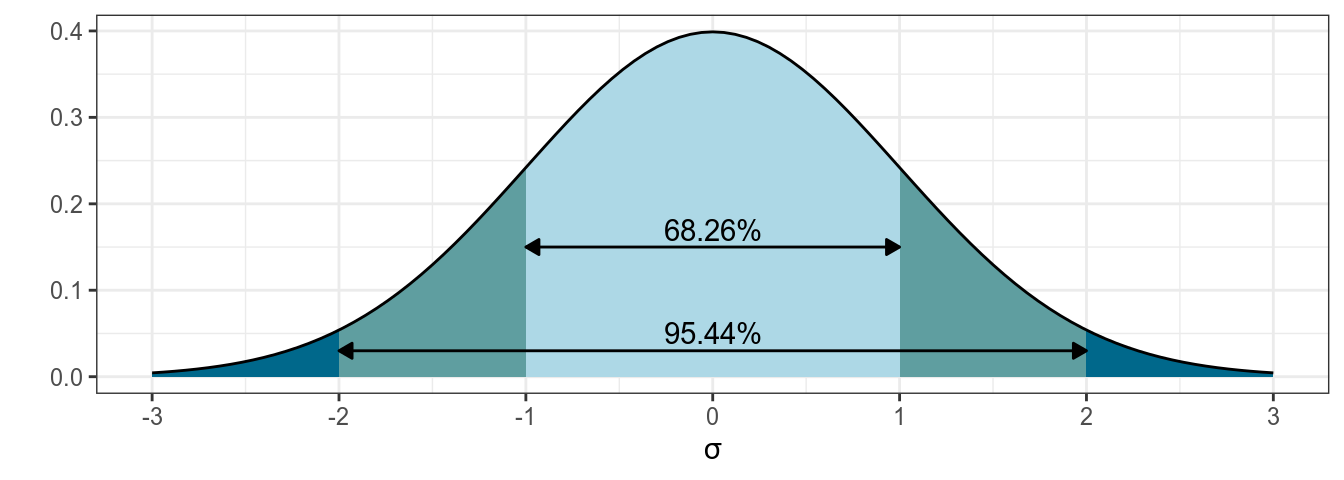
\includegraphics{da4l_files/figure-latex/unnamed-chunk-3-1.pdf}

\begin{Shaded}
\begin{Highlighting}[]
\FunctionTok{tibble}\NormalTok{(}\AttributeTok{x =} \DecValTok{1}\SpecialCharTok{:}\DecValTok{100}\NormalTok{,}
       \AttributeTok{CDF =} \FunctionTok{pnorm}\NormalTok{(x, }\AttributeTok{mean =} \DecValTok{50}\NormalTok{, }\AttributeTok{sd =} \DecValTok{10}\NormalTok{)) }\SpecialCharTok{\%\textgreater{}\%} 
  \FunctionTok{ggplot}\NormalTok{(}\FunctionTok{aes}\NormalTok{(x, CDF))}\SpecialCharTok{+}
  \FunctionTok{geom\_point}\NormalTok{()}\SpecialCharTok{+}
  \FunctionTok{geom\_line}\NormalTok{()}\SpecialCharTok{+}
  \FunctionTok{labs}\NormalTok{(}\AttributeTok{title =} \StringTok{"CDF нормального распределения (μ = 50, sd = 10)"}\NormalTok{)}
\end{Highlighting}
\end{Shaded}

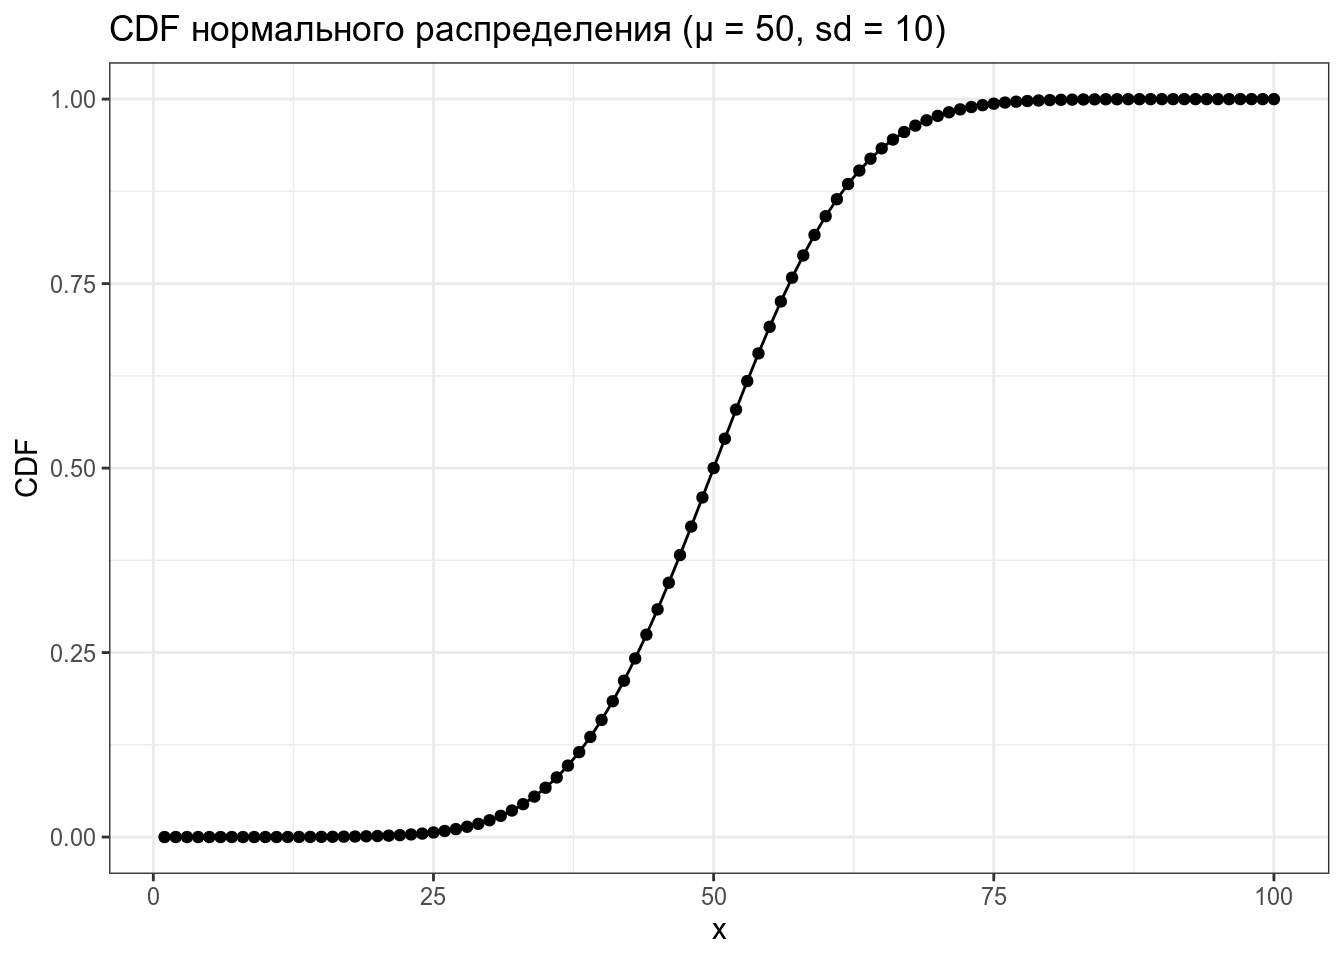
\includegraphics{da4l_files/figure-latex/unnamed-chunk-3-2.pdf}

\begin{Shaded}
\begin{Highlighting}[]
\FunctionTok{tibble}\NormalTok{(}\AttributeTok{quantiles =} \FunctionTok{seq}\NormalTok{(}\DecValTok{0}\NormalTok{, }\DecValTok{1}\NormalTok{, }\AttributeTok{by =} \FloatTok{0.01}\NormalTok{),}
       \AttributeTok{value =} \FunctionTok{qnorm}\NormalTok{(quantiles, }\AttributeTok{mean =} \DecValTok{50}\NormalTok{, }\AttributeTok{sd =} \DecValTok{10}\NormalTok{)) }\SpecialCharTok{\%\textgreater{}\%} 
  \FunctionTok{ggplot}\NormalTok{(}\FunctionTok{aes}\NormalTok{(quantiles, value))}\SpecialCharTok{+}
  \FunctionTok{geom\_point}\NormalTok{()}\SpecialCharTok{+}
  \FunctionTok{geom\_line}\NormalTok{()}\SpecialCharTok{+}
  \FunctionTok{labs}\NormalTok{(}\AttributeTok{title =} \StringTok{"inverse CDF нормального распределения (μ = 50, sd = 10)"}\NormalTok{)}
\end{Highlighting}
\end{Shaded}

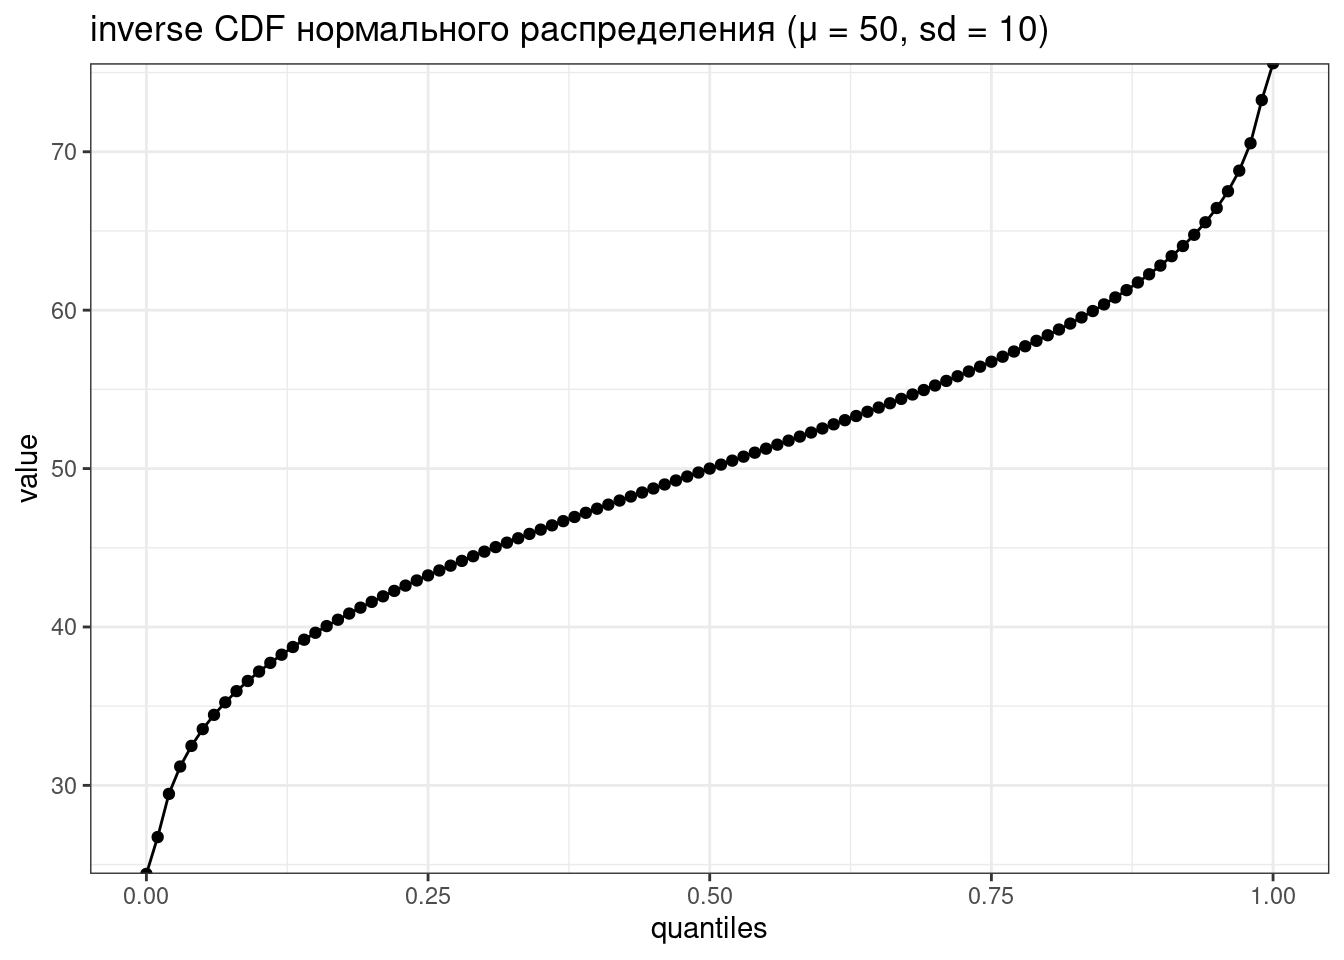
\includegraphics{da4l_files/figure-latex/unnamed-chunk-3-3.pdf}

\begin{Shaded}
\begin{Highlighting}[]
\FunctionTok{tibble}\NormalTok{(}\AttributeTok{sample =} \FunctionTok{rnorm}\NormalTok{(}\DecValTok{100}\NormalTok{, }\AttributeTok{mean =} \DecValTok{50}\NormalTok{, }\AttributeTok{sd =} \DecValTok{10}\NormalTok{)) }\SpecialCharTok{\%\textgreater{}\%} 
  \FunctionTok{ggplot}\NormalTok{(}\FunctionTok{aes}\NormalTok{(sample))}\SpecialCharTok{+}
  \FunctionTok{geom\_histogram}\NormalTok{()}\SpecialCharTok{+}
  \FunctionTok{labs}\NormalTok{(}\AttributeTok{title =} \StringTok{"выборка нормально распределенных чисел (μ = 50, sd = 10)"}\NormalTok{)}
\end{Highlighting}
\end{Shaded}

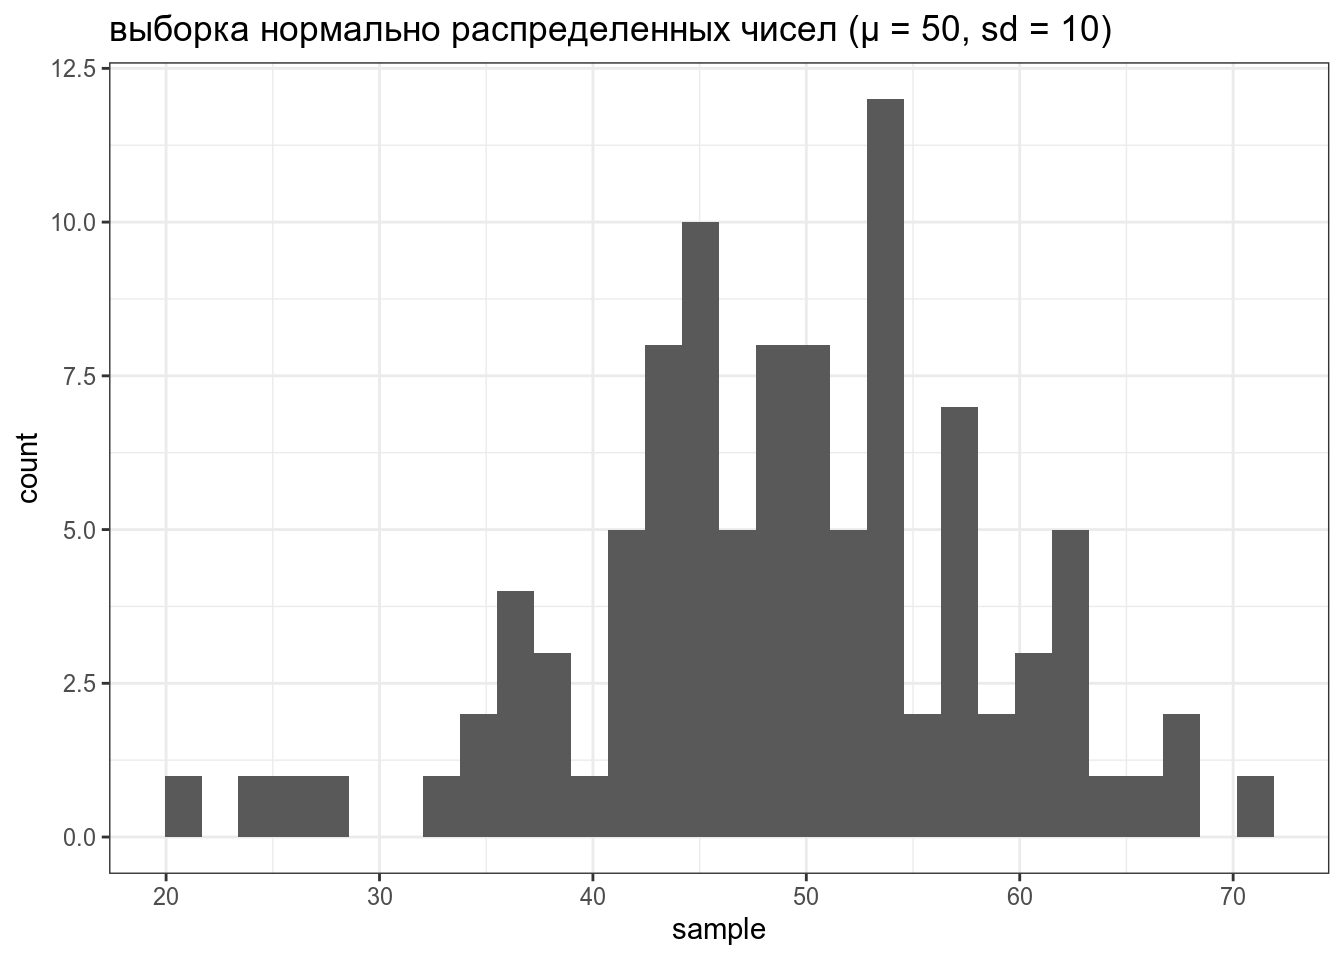
\includegraphics{da4l_files/figure-latex/unnamed-chunk-3-4.pdf}

Если не использовать \texttt{set.seed()}, то результат работы рандомизатора нельзя будет повторить.

\begin{rmdtask}
Какое значение имеет 25\% квантиль нормального распределения со средним
в 20 и стандартным отклонением 90? Ответ округлите до трех знаков после
запятой.
\end{rmdtask}

\begin{rmdtask}
Данные из базы данных фонетических инвентарей PHOIBLE {[}@phoible{]},
достаточно сильно упрощая, можно описать нормальным распределением со
средним 35 фонем и стандартным отклонением 13. Если мы ничего не знаем
про язык, оцените с какой вероятностью, согласно этой модели произвольно
взятый язык окажется в промежутке между 25 и 50 фонемами? Ответ
округлите до трех знаков после запятой.
\end{rmdtask}

\begin{rmdtask}
Какие есть недостатки у модели из предыдущего задания?
\end{rmdtask}

\hypertarget{ux434ux438ux441ux43aux440ux435ux442ux43dux44bux435-ux43fux435ux440ux435ux43cux435ux43dux43dux44bux435}{%
\section{Дискретные переменные}\label{ux434ux438ux441ux43aux440ux435ux442ux43dux44bux435-ux43fux435ux440ux435ux43cux435ux43dux43dux44bux435}}

\hypertarget{ux431ux438ux43dux43eux43cux438ux430ux43bux44cux43dux43eux435-ux440ux430ux441ux43fux440ux435ux434ux435ux43bux435ux43dux438ux435}{%
\subsection{Биномиальное распределение}\label{ux431ux438ux43dux43eux43cux438ux430ux43bux44cux43dux43eux435-ux440ux430ux441ux43fux440ux435ux434ux435ux43bux435ux43dux438ux435}}

Биномиальное распределение --- распределение количетсва успехов эксперементов Бернулли из \emph{n} попыток с вероятностью успеха \emph{p}.

\[P(k | n, p) = \frac{n!}{k!(n-k)!} \times p^k \times (1-p)^{n-k} =  {n \choose k} \times p^k \times (1-p)^{n-k}\]
\[ 0 \leq p \leq 1; n, k > 0\]

\begin{Shaded}
\begin{Highlighting}[]
\FunctionTok{tibble}\NormalTok{(}\AttributeTok{x =} \DecValTok{0}\SpecialCharTok{:}\DecValTok{50}\NormalTok{,}
       \AttributeTok{density =} \FunctionTok{dbinom}\NormalTok{(}\AttributeTok{x =}\NormalTok{ x, }\AttributeTok{size =} \DecValTok{50}\NormalTok{, }\AttributeTok{prob =} \FloatTok{0.16}\NormalTok{)) }\SpecialCharTok{\%\textgreater{}\%} 
  \FunctionTok{ggplot}\NormalTok{(}\FunctionTok{aes}\NormalTok{(x, density))}\SpecialCharTok{+}
  \FunctionTok{geom\_point}\NormalTok{()}\SpecialCharTok{+}
  \FunctionTok{geom\_line}\NormalTok{()}\SpecialCharTok{+}
  \FunctionTok{labs}\NormalTok{(}\AttributeTok{title =} \StringTok{"Биномиальное распределение p = 0.16, n = 50"}\NormalTok{)}
\end{Highlighting}
\end{Shaded}

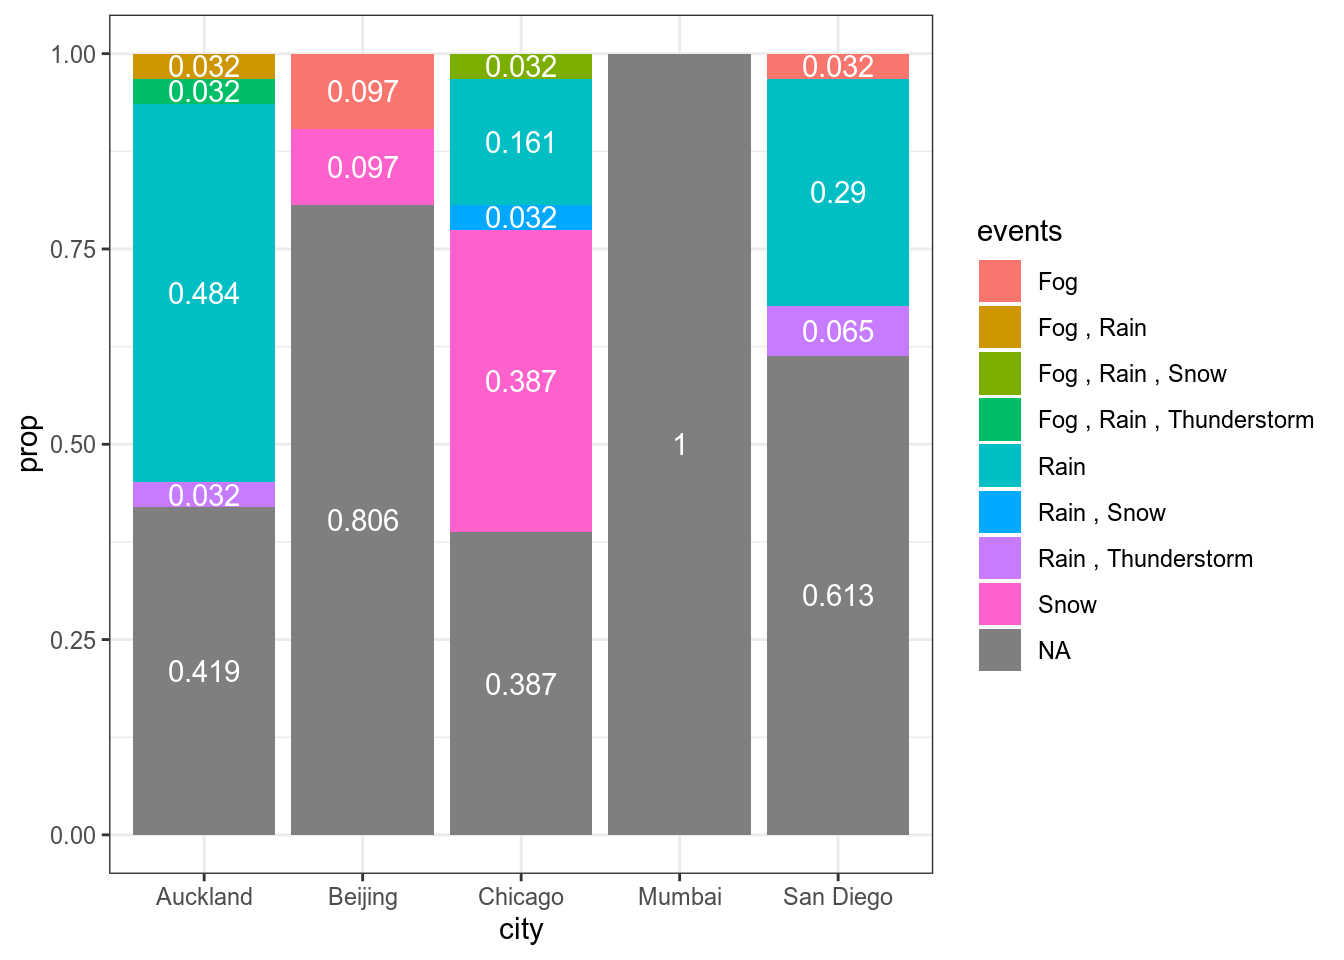
\includegraphics{da4l_files/figure-latex/unnamed-chunk-10-1.pdf}

\begin{rmdtask}
Немного упрощая данные из статьи {[}@rosenbach03: 394{]}, можно сказать
что носители британского английского предпочитают \emph{s}-генитив
(90\%) \emph{of}-генитиву (10\%). Какова вероятность, согласно этим
данным, что в интервью британского актера из 118 контекстов будет 102
\emph{s}-генитивов? Ответ округлите до трёх или менее знаков после
запятой.
\end{rmdtask}

\begin{rmdtask}
А какое значение количества \emph{s}-генитивов наиболее ожидаемо,
согласно этой модели?
\end{rmdtask}

\hypertarget{ux433ux435ux43eux43cux435ux442ux440ux438ux447ux435ux441ux43aux43eux435-ux440ux430ux441ux43fux440ux435ux434ux435ux43bux435ux43dux438ux435}{%
\subsection{Геометрическое распределение}\label{ux433ux435ux43eux43cux435ux442ux440ux438ux447ux435ux441ux43aux43eux435-ux440ux430ux441ux43fux440ux435ux434ux435ux43bux435ux43dux438ux435}}

Геометрическое распределение --- распределение количетсва эксперементов Бернулли с вероятностью успеха \emph{p} до первого успеха.

\[P(k | p) = (1-p)^k\times p\]
\[k\in\{1, 2, \dots\}\]

\begin{Shaded}
\begin{Highlighting}[]
\FunctionTok{tibble}\NormalTok{(}\AttributeTok{x =} \DecValTok{0}\SpecialCharTok{:}\DecValTok{50}\NormalTok{,}
       \AttributeTok{density =} \FunctionTok{dgeom}\NormalTok{(}\AttributeTok{x =}\NormalTok{ x, }\AttributeTok{prob =} \FloatTok{0.16}\NormalTok{)) }\SpecialCharTok{\%\textgreater{}\%} 
  \FunctionTok{ggplot}\NormalTok{(}\FunctionTok{aes}\NormalTok{(x, density))}\SpecialCharTok{+}
  \FunctionTok{geom\_point}\NormalTok{()}\SpecialCharTok{+}
  \FunctionTok{geom\_line}\NormalTok{()}\SpecialCharTok{+}
  \FunctionTok{labs}\NormalTok{(}\AttributeTok{title =} \StringTok{"Геометрическое распределение p = 0.16, n = 50"}\NormalTok{)}
\end{Highlighting}
\end{Shaded}

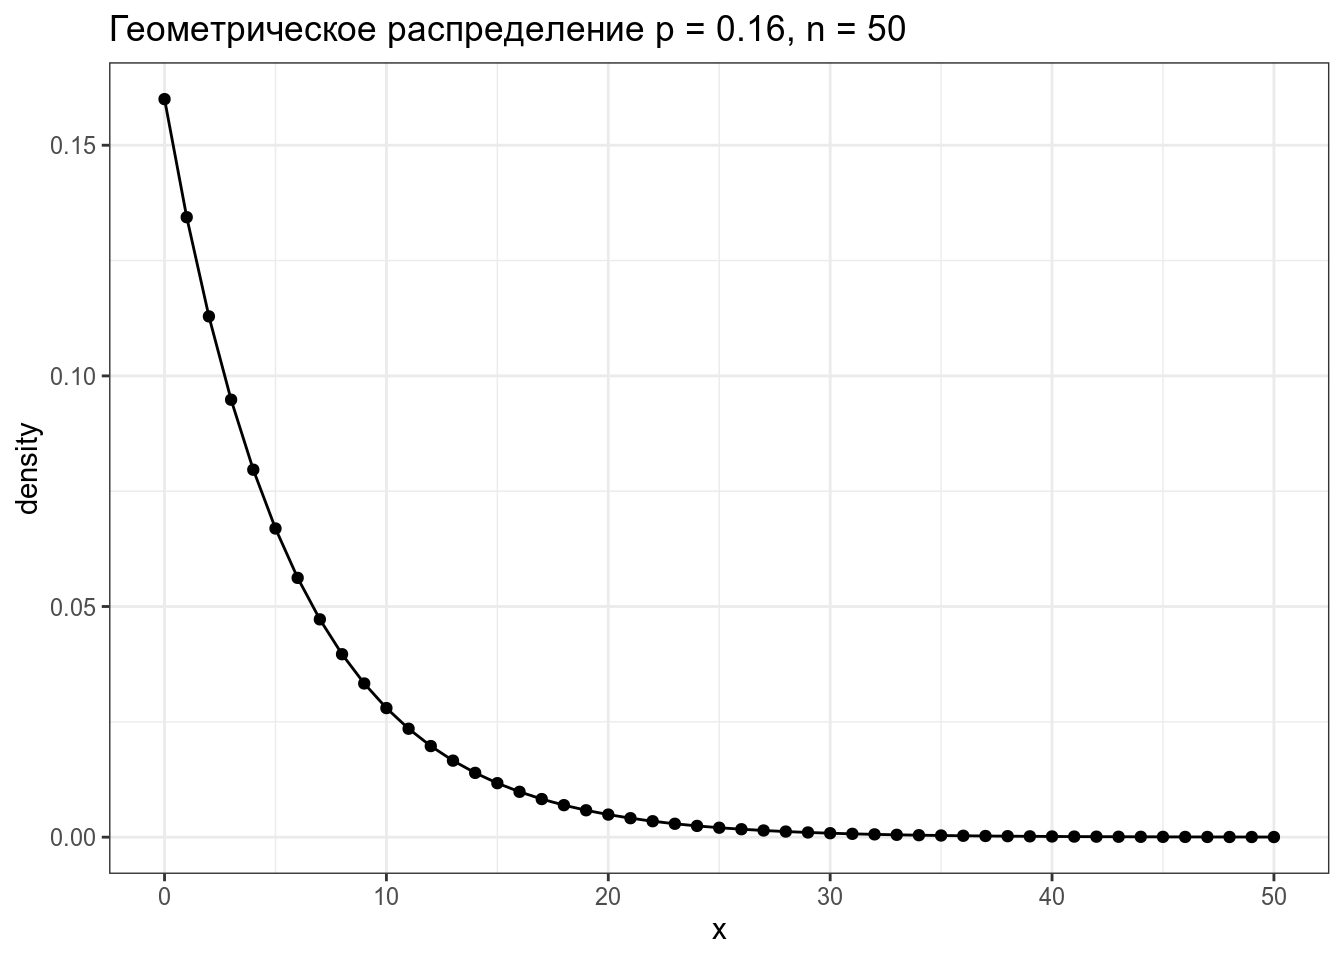
\includegraphics{da4l_files/figure-latex/unnamed-chunk-15-1.pdf}

\begin{rmdtask}
Приняв модель из {[}@rosenbach03: 394{]}, какова вероятность, что в
интервью с британским актером первый \emph{of}-генитив будет третьим по
счету?
\end{rmdtask}

\hypertarget{ux440ux430ux441ux43fux440ux435ux434ux435ux43bux435ux43dux438ux435-ux43fux443ux430ux441ux441ux43eux43dux430}{%
\subsection{Распределение Пуассона}\label{ux440ux430ux441ux43fux440ux435ux434ux435ux43bux435ux43dux438ux435-ux43fux443ux430ux441ux441ux43eux43dux430}}

Распределение дискретной переменной, обозначающей количество случаев \(k\) некоторого события, которое происходит с некоторой заданной частотой \(\lambda\).

\[P(\lambda) = \frac{e^{-\lambda}\times\lambda^k}{k!}\]

\begin{Shaded}
\begin{Highlighting}[]
\FunctionTok{tibble}\NormalTok{(}\AttributeTok{k =} \DecValTok{0}\SpecialCharTok{:}\DecValTok{50}\NormalTok{,}
       \AttributeTok{density =} \FunctionTok{dpois}\NormalTok{(}\AttributeTok{x =}\NormalTok{ k, }\AttributeTok{lambda =} \DecValTok{5}\NormalTok{)) }\SpecialCharTok{\%\textgreater{}\%} 
  \FunctionTok{ggplot}\NormalTok{(}\FunctionTok{aes}\NormalTok{(k, density))}\SpecialCharTok{+}
  \FunctionTok{geom\_point}\NormalTok{()}\SpecialCharTok{+}
  \FunctionTok{geom\_line}\NormalTok{()}\SpecialCharTok{+}
  \FunctionTok{labs}\NormalTok{(}\AttributeTok{title =} \StringTok{"Распределение Пуассона с параметром λ = 5"}\NormalTok{)}
\end{Highlighting}
\end{Shaded}

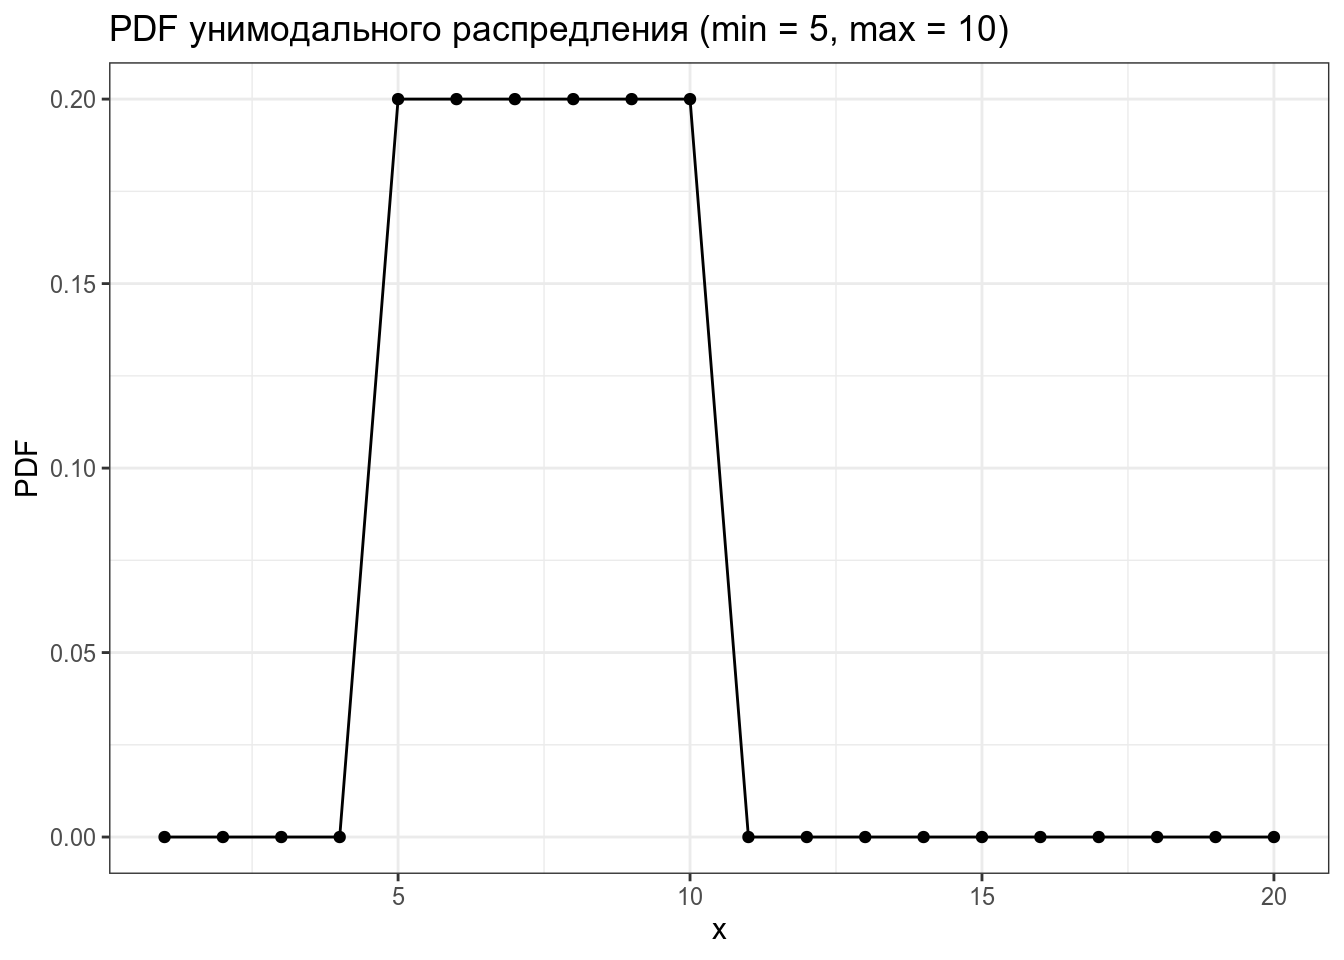
\includegraphics{da4l_files/figure-latex/unnamed-chunk-18-1.pdf}

Параметр \(\lambda\) в модели Пуассона одновременно является и средним, и дисперсией.

Попробуем воспользоваться распределением Пуассона для моделирования количества слогов в андийском языке. Количество слогов -- это всегда натуральное число (т. е. не бывает 2.5 слогов, не бывает -3 слогов и т. д., но в теории может быть 0 слогов), так что модель Пуассона здесь применима. Согласно модели Пуассона все слова независимо друг от друга получают сколько-то слогов согласно распределению Пуассона. Посмотрим на данные:

\begin{Shaded}
\begin{Highlighting}[]
\NormalTok{andic\_syllables }\OtherTok{\textless{}{-}} \FunctionTok{read\_csv}\NormalTok{(}\StringTok{"https://raw.githubusercontent.com/agricolamz/2021\_da4l/master/data/andic\_syllables.csv"}\NormalTok{) }

\NormalTok{andic\_syllables }\SpecialCharTok{\%\textgreater{}\%} 
  \FunctionTok{ggplot}\NormalTok{(}\FunctionTok{aes}\NormalTok{(n\_syllables, count))}\SpecialCharTok{+}
  \FunctionTok{geom\_col}\NormalTok{()}\SpecialCharTok{+}
  \FunctionTok{facet\_wrap}\NormalTok{(}\SpecialCharTok{\textasciitilde{}}\NormalTok{language, }\AttributeTok{scales =} \StringTok{"free"}\NormalTok{)}
\end{Highlighting}
\end{Shaded}

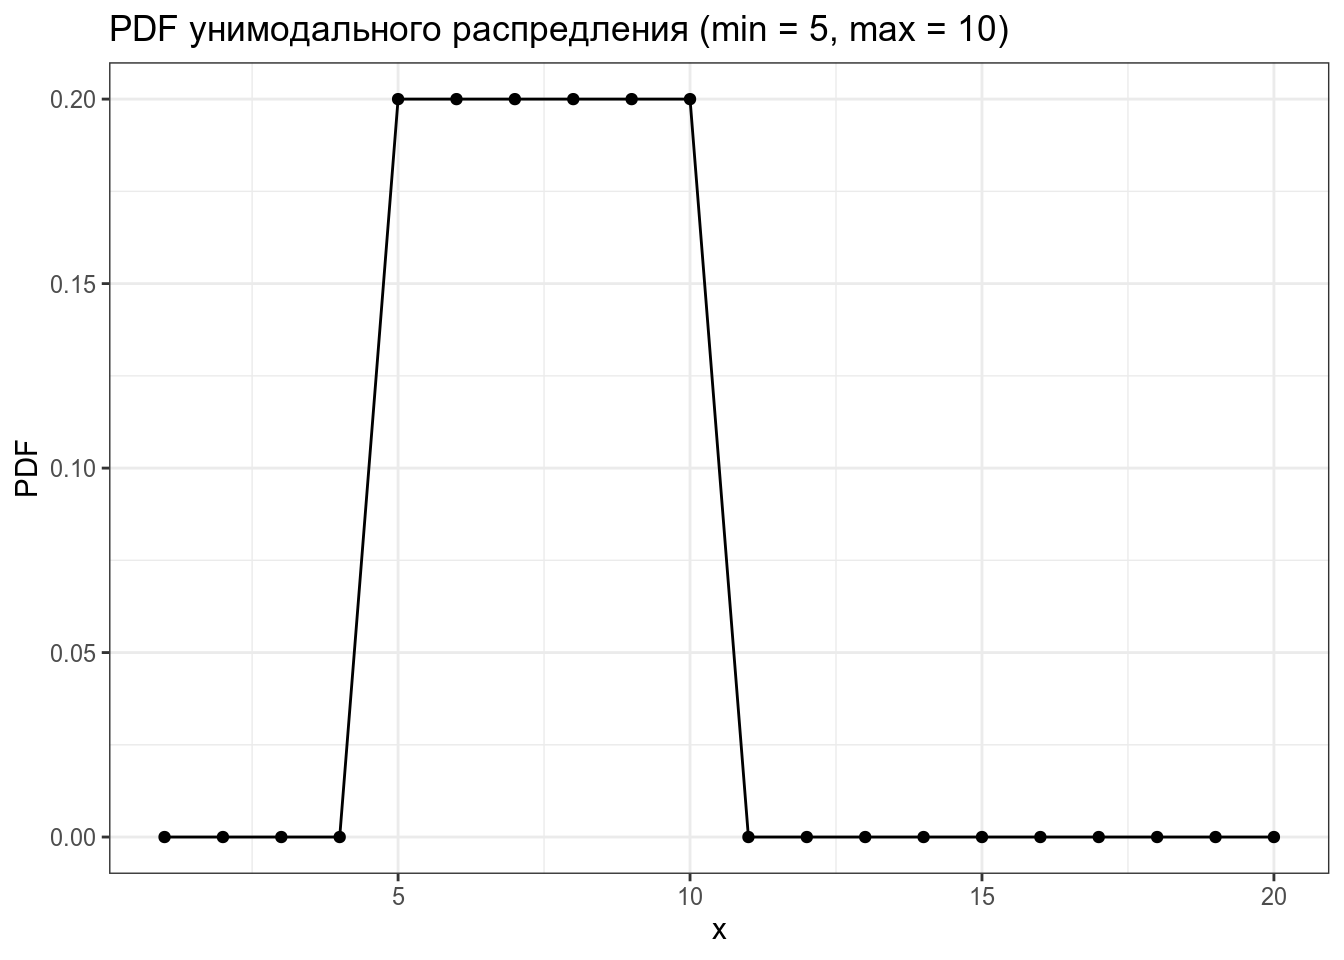
\includegraphics{da4l_files/figure-latex/unnamed-chunk-19-1.pdf}

Птичка напела (мы научимся узнавать, откуда птичка это знает на следующем занятии), что андийские данные можно описать при помощи распределения Пуассона с параметром \(\lambda\) = 2.783.

\begin{Shaded}
\begin{Highlighting}[]
\NormalTok{andic\_syllables }\SpecialCharTok{\%\textgreater{}\%} 
  \FunctionTok{filter}\NormalTok{(language }\SpecialCharTok{==} \StringTok{"Andi"}\NormalTok{) }\SpecialCharTok{\%\textgreater{}\%} 
  \FunctionTok{rename}\NormalTok{(}\AttributeTok{observed =}\NormalTok{ count) }\SpecialCharTok{\%\textgreater{}\%} 
  \FunctionTok{mutate}\NormalTok{(}\AttributeTok{predicted =} \FunctionTok{dpois}\NormalTok{(n\_syllables, }\AttributeTok{lambda =} \FloatTok{2.783}\NormalTok{)}\SpecialCharTok{*}\FunctionTok{sum}\NormalTok{(observed)) }\SpecialCharTok{\%\textgreater{}\%} 
  \FunctionTok{pivot\_longer}\NormalTok{(}\AttributeTok{names\_to =} \StringTok{"type"}\NormalTok{, }\AttributeTok{values\_to =} \StringTok{"value"}\NormalTok{, }\AttributeTok{cols =} \FunctionTok{c}\NormalTok{(observed, predicted)) }\SpecialCharTok{\%\textgreater{}\%} 
  \FunctionTok{ggplot}\NormalTok{(}\FunctionTok{aes}\NormalTok{(n\_syllables, value, }\AttributeTok{fill =}\NormalTok{ type))}\SpecialCharTok{+}
  \FunctionTok{geom\_col}\NormalTok{(}\AttributeTok{position =} \StringTok{"dodge"}\NormalTok{)}
\end{Highlighting}
\end{Shaded}

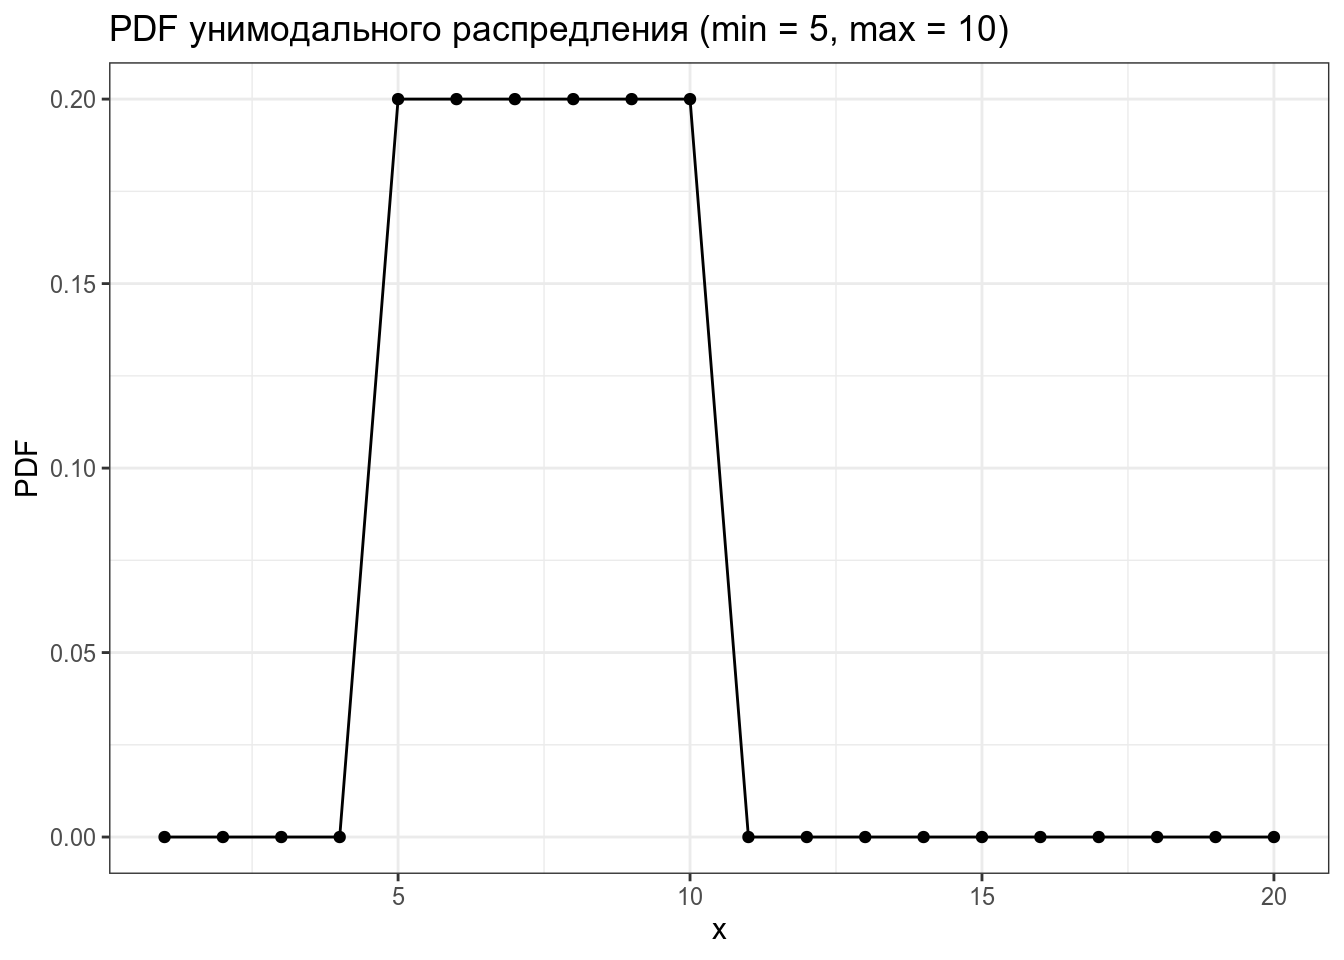
\includegraphics{da4l_files/figure-latex/unnamed-chunk-21-1.pdf}

\begin{rmdtask}
На графиках ниже представлены предсказания трех Пуассоновских моделей,
какая кажется лучше?
\end{rmdtask}

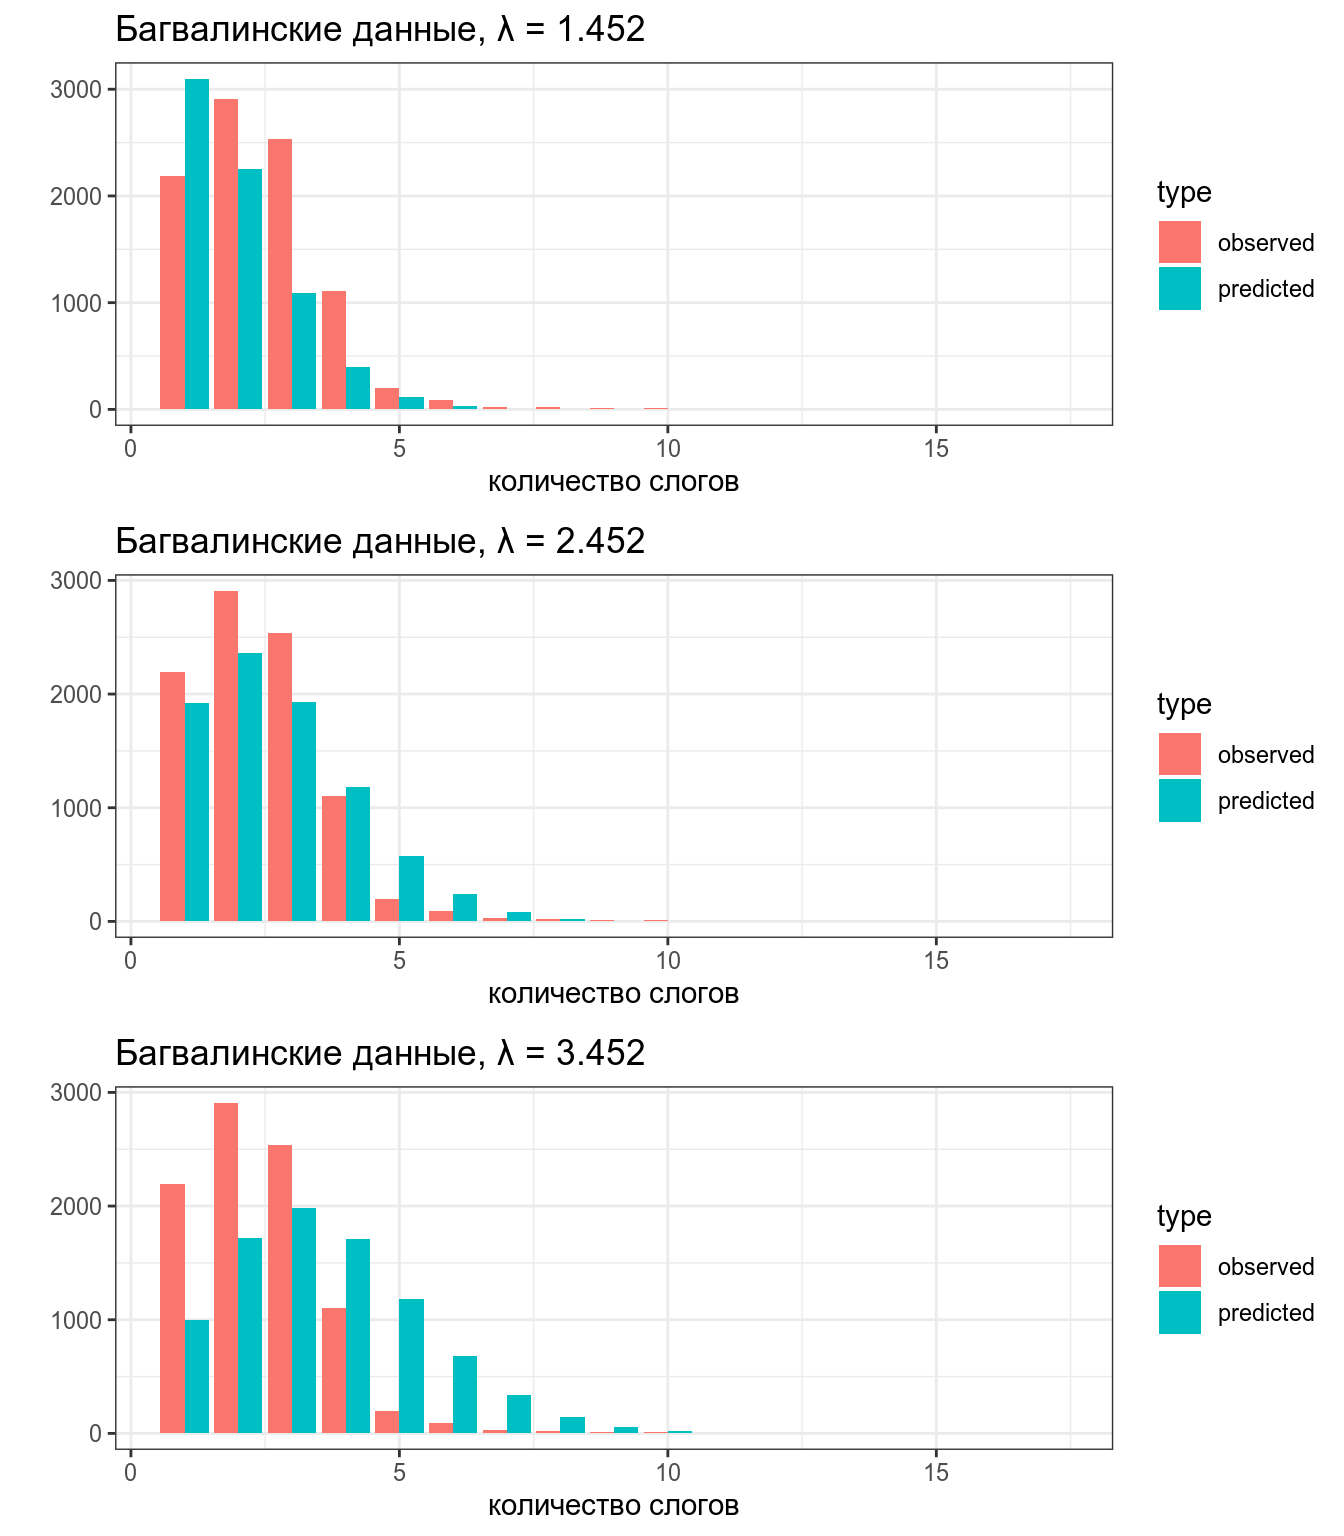
\includegraphics{da4l_files/figure-latex/unnamed-chunk-23-1.pdf}

\begin{rmdtask}
Выше было написано:

\begin{quote}
Согласно модели Пуассона все слова \textbf{независимо друг от друга}
получают сколько-то слогов согласно распределению Пуассона.
\end{quote}

Какие проблемы есть у предположения о независимости друг от друга
количества слогов разных слов в словаре?
\end{rmdtask}

\hypertarget{ux447ux438ux441ux43bux43eux432ux44bux435-ux43fux435ux440ux435ux43cux435ux43dux43dux44bux435}{%
\section{Числовые переменные}\label{ux447ux438ux441ux43bux43eux432ux44bux435-ux43fux435ux440ux435ux43cux435ux43dux43dux44bux435}}

\hypertarget{ux43dux43eux440ux43cux430ux43bux44cux43dux43eux435-ux440ux430ux441ux43fux440ux435ux434ux435ux43bux435ux43dux438ux435}{%
\subsection{Нормальное распределение}\label{ux43dux43eux440ux43cux430ux43bux44cux43dux43eux435-ux440ux430ux441ux43fux440ux435ux434ux435ux43bux435ux43dux438ux435}}

\[P(x) = \frac{1}{\sigma\sqrt{2\pi}}\times e^{-\frac{\left(x-\mu\right)^2}{2\sigma^2}}\]

\[\mu \in \mathbb{R}; \sigma^2 > 0\]

\begin{Shaded}
\begin{Highlighting}[]
\FunctionTok{tibble}\NormalTok{(}\AttributeTok{x =} \DecValTok{1}\SpecialCharTok{:}\DecValTok{100}\NormalTok{,}
       \AttributeTok{PDF =} \FunctionTok{dnorm}\NormalTok{(}\AttributeTok{x =}\NormalTok{ x, }\AttributeTok{mean =} \DecValTok{50}\NormalTok{, }\AttributeTok{sd =} \DecValTok{10}\NormalTok{)) }\SpecialCharTok{\%\textgreater{}\%} 
  \FunctionTok{ggplot}\NormalTok{(}\FunctionTok{aes}\NormalTok{(x, PDF))}\SpecialCharTok{+}
  \FunctionTok{geom\_point}\NormalTok{()}\SpecialCharTok{+}
  \FunctionTok{geom\_line}\NormalTok{()}\SpecialCharTok{+}
  \FunctionTok{labs}\NormalTok{(}\AttributeTok{title =} \StringTok{"PDF нормального распределения (μ = 50, sd = 10)"}\NormalTok{)}
\end{Highlighting}
\end{Shaded}

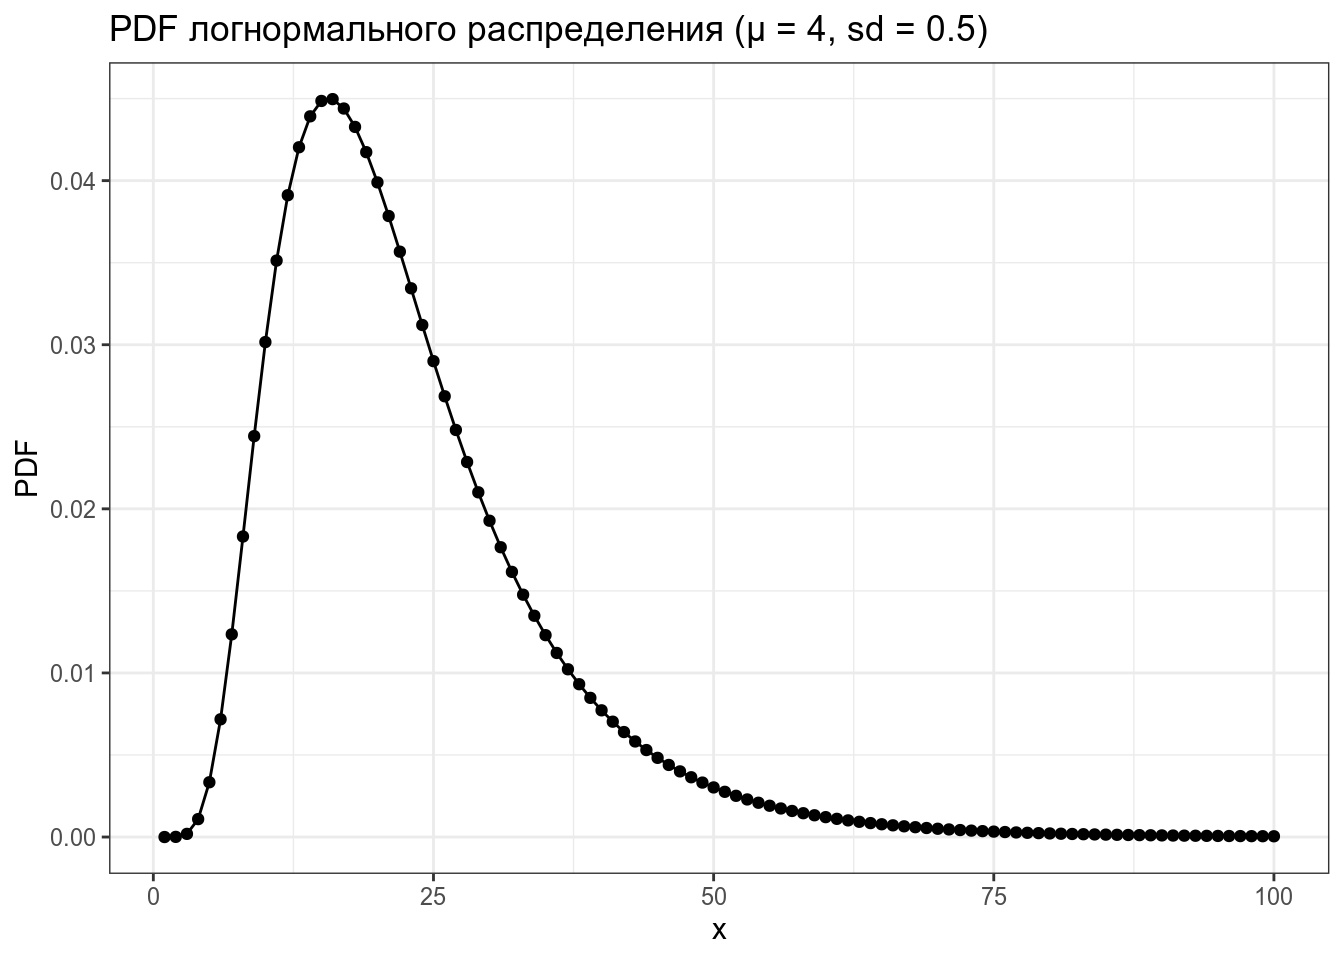
\includegraphics{da4l_files/figure-latex/unnamed-chunk-25-1.pdf}

Птичка напела, что длительность гласных американского английского из \citep{hillenbrand95} можно описать нормальным распределением с параметрами \(\mu =\) 274.673 и \(\sigma =\) 64.482. Посмотрим, как можно совместить данные и это распределение:

\begin{Shaded}
\begin{Highlighting}[]
\NormalTok{vowels }\OtherTok{\textless{}{-}} \FunctionTok{read\_csv}\NormalTok{(}\StringTok{"https://raw.githubusercontent.com/agricolamz/2021\_da4l/master/data/phonTools\_hillenbrand\_1995.csv"}\NormalTok{) }
\NormalTok{vowels }\SpecialCharTok{\%\textgreater{}\%} 
  \FunctionTok{ggplot}\NormalTok{(}\FunctionTok{aes}\NormalTok{(dur)) }\SpecialCharTok{+} 
  \FunctionTok{geom\_histogram}\NormalTok{(}\FunctionTok{aes}\NormalTok{(}\AttributeTok{y =}\NormalTok{..density..)) }\SpecialCharTok{+} \CommentTok{\# обратите внимание на аргумент ..density..}
  \FunctionTok{stat\_function}\NormalTok{(}\AttributeTok{fun =}\NormalTok{ dnorm, }\AttributeTok{args =} \FunctionTok{list}\NormalTok{(}\AttributeTok{mean =} \FloatTok{274.673}\NormalTok{, }\AttributeTok{sd =} \FloatTok{64.482}\NormalTok{), }\AttributeTok{color =} \StringTok{"red"}\NormalTok{)}
\end{Highlighting}
\end{Shaded}

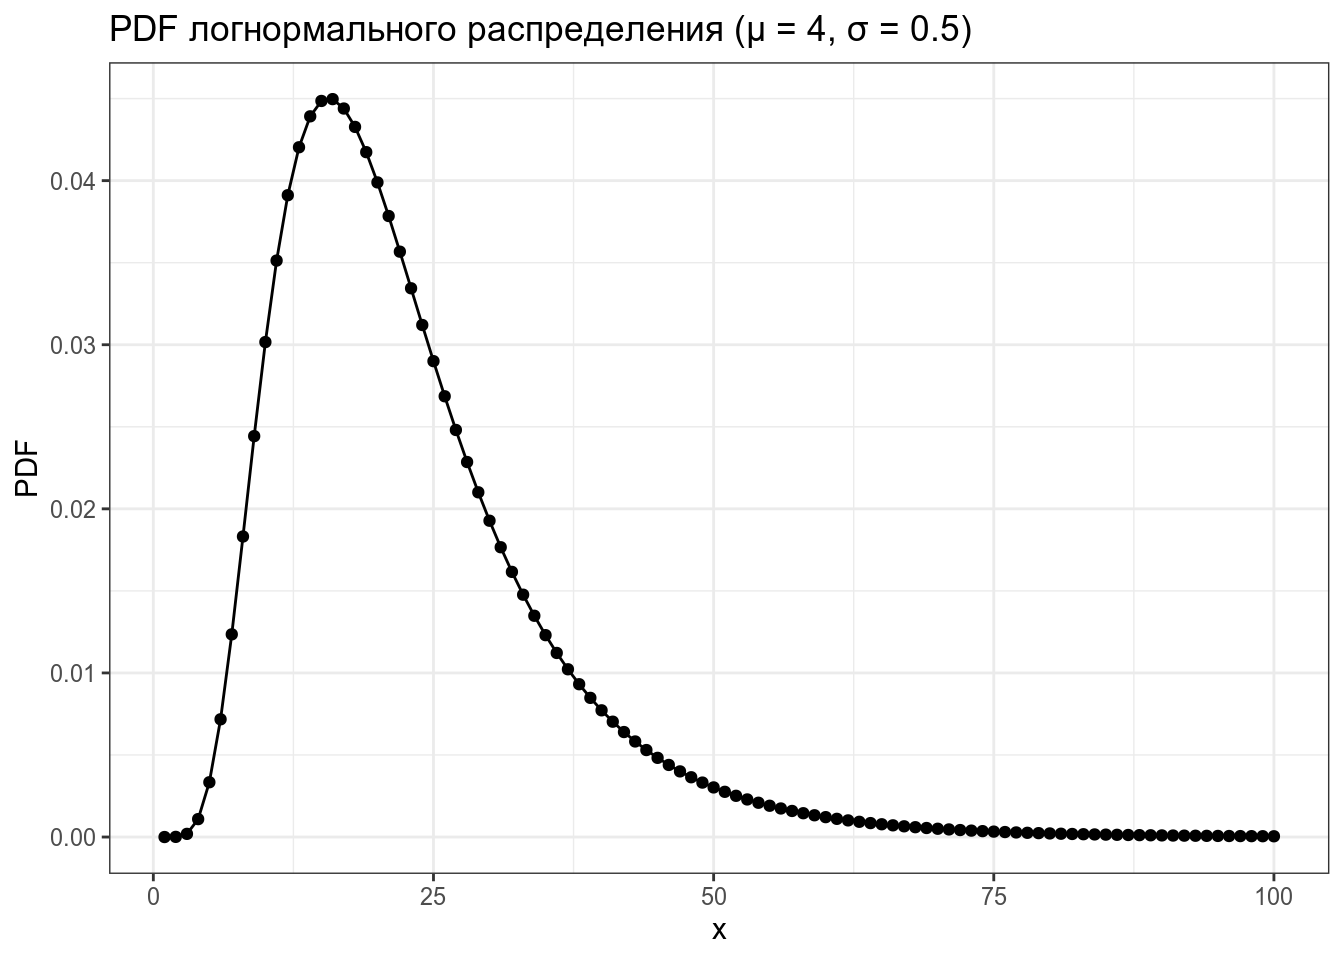
\includegraphics{da4l_files/figure-latex/unnamed-chunk-27-1.pdf}

\hypertarget{ux43bux43eux433ux43dux43eux440ux43cux430ux43bux44cux43dux43eux435-ux440ux430ux441ux43fux440ux435ux434ux435ux43bux435ux43dux438ux435}{%
\subsection{Логнормальное распределение}\label{ux43bux43eux433ux43dux43eux440ux43cux430ux43bux44cux43dux43eux435-ux440ux430ux441ux43fux440ux435ux434ux435ux43bux435ux43dux438ux435}}

\[P(x) = \frac{1}{\sqrt{x\sigma2\pi}}\times e^{-\frac{\left(\ln(x)-\mu\right)^2}{2\sigma^2}}\]

\[\mu \in \mathbb{R}; \sigma^2 > 0\]

\begin{Shaded}
\begin{Highlighting}[]
\FunctionTok{tibble}\NormalTok{(}\AttributeTok{x =} \DecValTok{1}\SpecialCharTok{:}\DecValTok{100}\NormalTok{,}
       \AttributeTok{PDF =} \FunctionTok{dlnorm}\NormalTok{(}\AttributeTok{x =}\NormalTok{ x, }\AttributeTok{mean =} \DecValTok{3}\NormalTok{, }\AttributeTok{sd =} \FloatTok{0.5}\NormalTok{)) }\SpecialCharTok{\%\textgreater{}\%} 
  \FunctionTok{ggplot}\NormalTok{(}\FunctionTok{aes}\NormalTok{(x, PDF))}\SpecialCharTok{+}
  \FunctionTok{geom\_point}\NormalTok{()}\SpecialCharTok{+}
  \FunctionTok{geom\_line}\NormalTok{()}\SpecialCharTok{+}
  \FunctionTok{labs}\NormalTok{(}\AttributeTok{title =} \StringTok{"PDF логнормального распределения (μ = 3, σ = 0.5)"}\NormalTok{)}
\end{Highlighting}
\end{Shaded}

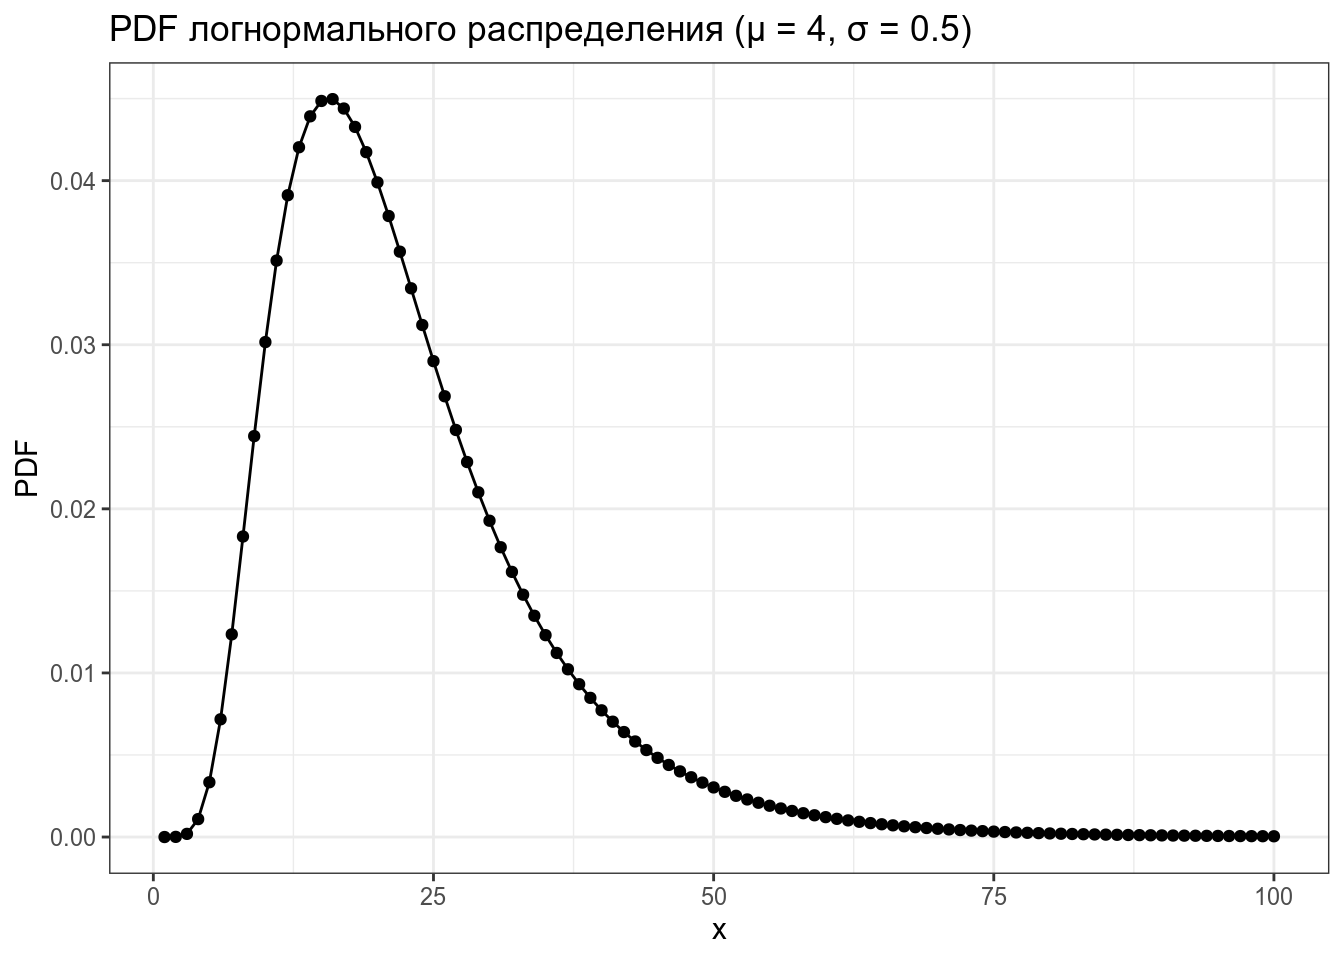
\includegraphics{da4l_files/figure-latex/unnamed-chunk-28-1.pdf}

\begin{rmdtask}
Какая из логнормальных моделей для длительности гласных американского
английского из {[}@hillenbrand95{]} лучше подходит к данным? Попробуйте
самостоятельно построить данный график.
\end{rmdtask}

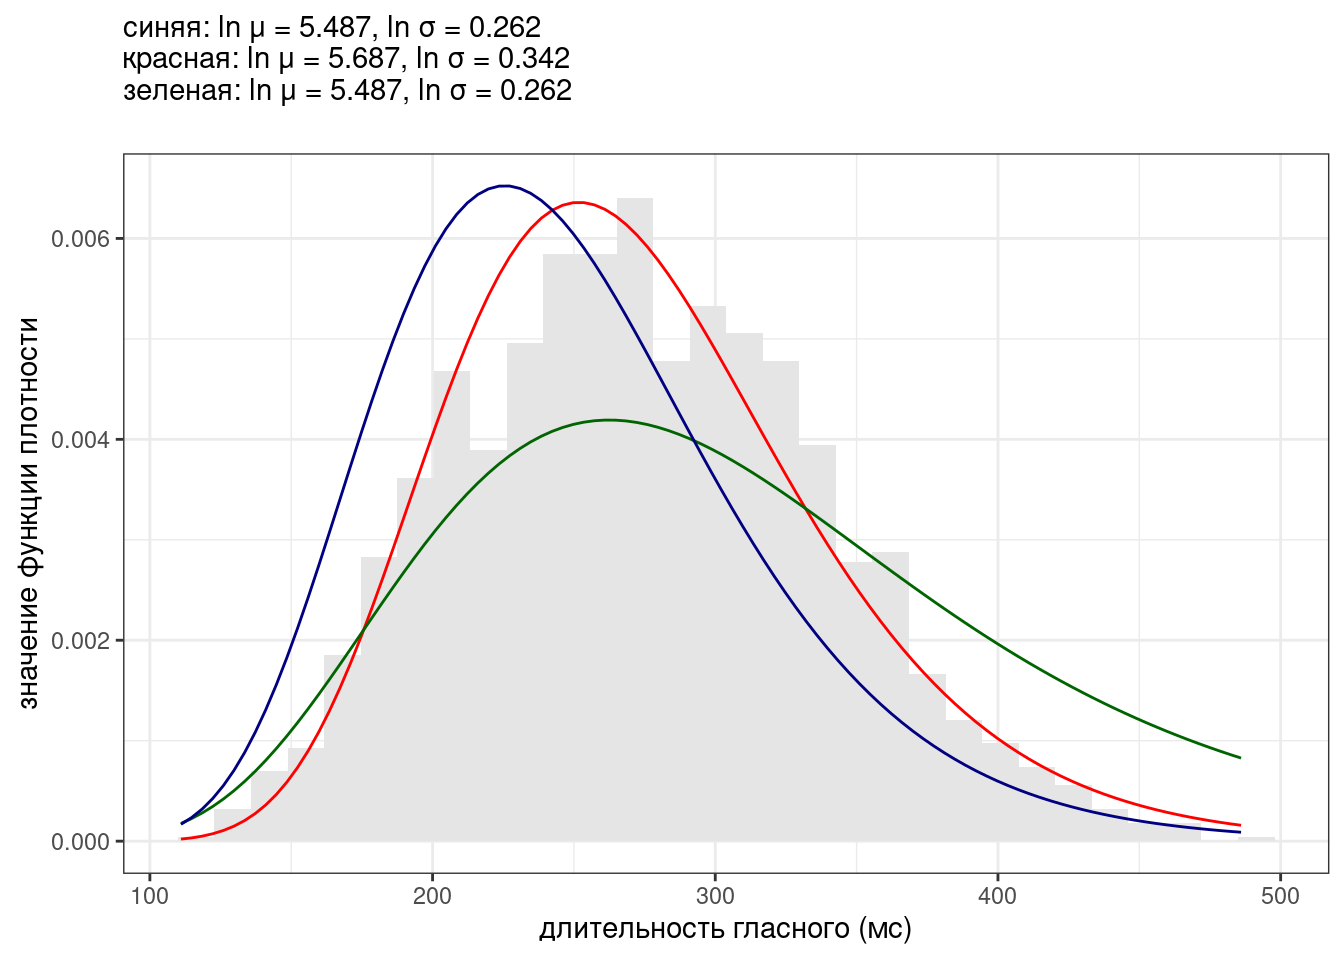
\includegraphics{da4l_files/figure-latex/unnamed-chunk-31-1.pdf}

\hypertarget{ux447ux442ux43e-ux435ux449ux435-ux43fux43eux447ux438ux442ux430ux442ux44c-ux43fux440ux43e-ux440ux430ux441ux43fux440ux435ux434ux435ux43bux435ux43dux438ux44f}{%
\subsection{Что еще почитать про распределения?}\label{ux447ux442ux43e-ux435ux449ux435-ux43fux43eux447ux438ux442ux430ux442ux44c-ux43fux440ux43e-ux440ux430ux441ux43fux440ux435ux434ux435ux43bux435ux43dux438ux44f}}

Люди придумали очень много разных распределений. Стоит, наверное, также понимать, что распределения не существуют отдельно в вакууме: многие из них математически связаны друг с другом. Про это можно посмотреть \href{http://www.math.wm.edu/~leemis/chart/UDR/UDR.html}{вот здесь} или \href{https://en.wikipedia.org/wiki/Relationships_among_probability_distributions}{здесь}.

\hypertarget{ux43cux435ux442ux43eux434-ux43cux430ux43aux441ux438ux43cux430ux43bux44cux43dux43eux433ux43e-ux43fux440ux430ux432ux434ux43eux43fux43eux434ux43eux431ux438ux44f}{%
\chapter{Метод максимального правдоподобия}\label{ux43cux435ux442ux43eux434-ux43cux430ux43aux441ux438ux43cux430ux43bux44cux43dux43eux433ux43e-ux43fux440ux430ux432ux434ux43eux43fux43eux434ux43eux431ux438ux44f}}

\hypertarget{ux43eux446ux435ux43dux43aux430-ux432ux435ux440ux43eux44fux442ux43dux43eux441ux442ux438}{%
\section{Оценка вероятности}\label{ux43eux446ux435ux43dux43aux430-ux432ux435ux440ux43eux44fux442ux43dux43eux441ux442ux438}}

\begin{Shaded}
\begin{Highlighting}[]
\FunctionTok{library}\NormalTok{(tidyverse)}
\end{Highlighting}
\end{Shaded}

Когда у нас задано некоторое распределение, мы можем задавать к нему разные вопросы. Например, если мы верим что длительность гласных американского английского из \citep{hillenbrand95} можно описать логнормальным распределением с параметрами \(\ln{\mu} =\) 5.587 и \(\ln{\sigma} =\) 0.242, то мы можем делать некотрые предсказания относительно интересующей нас переменной.

\begin{Shaded}
\begin{Highlighting}[]
\FunctionTok{ggplot}\NormalTok{() }\SpecialCharTok{+} 
  \FunctionTok{stat\_function}\NormalTok{(}\AttributeTok{fun =}\NormalTok{ dlnorm, }\AttributeTok{args =} \FunctionTok{list}\NormalTok{(}\AttributeTok{mean =} \FloatTok{5.587}\NormalTok{, }\AttributeTok{sd =} \FloatTok{0.242}\NormalTok{))}\SpecialCharTok{+}
  \FunctionTok{scale\_x\_continuous}\NormalTok{(}\AttributeTok{breaks =} \DecValTok{0}\SpecialCharTok{:}\DecValTok{6}\SpecialCharTok{*}\DecValTok{100}\NormalTok{, }\AttributeTok{limits =} \FunctionTok{c}\NormalTok{(}\DecValTok{0}\NormalTok{, }\DecValTok{650}\NormalTok{))}\SpecialCharTok{+}
  \FunctionTok{labs}\NormalTok{(}\AttributeTok{x =} \StringTok{"длительность гласного (мс)"}\NormalTok{,}
       \AttributeTok{y =} \StringTok{"значение функции плотности"}\NormalTok{)}
\end{Highlighting}
\end{Shaded}

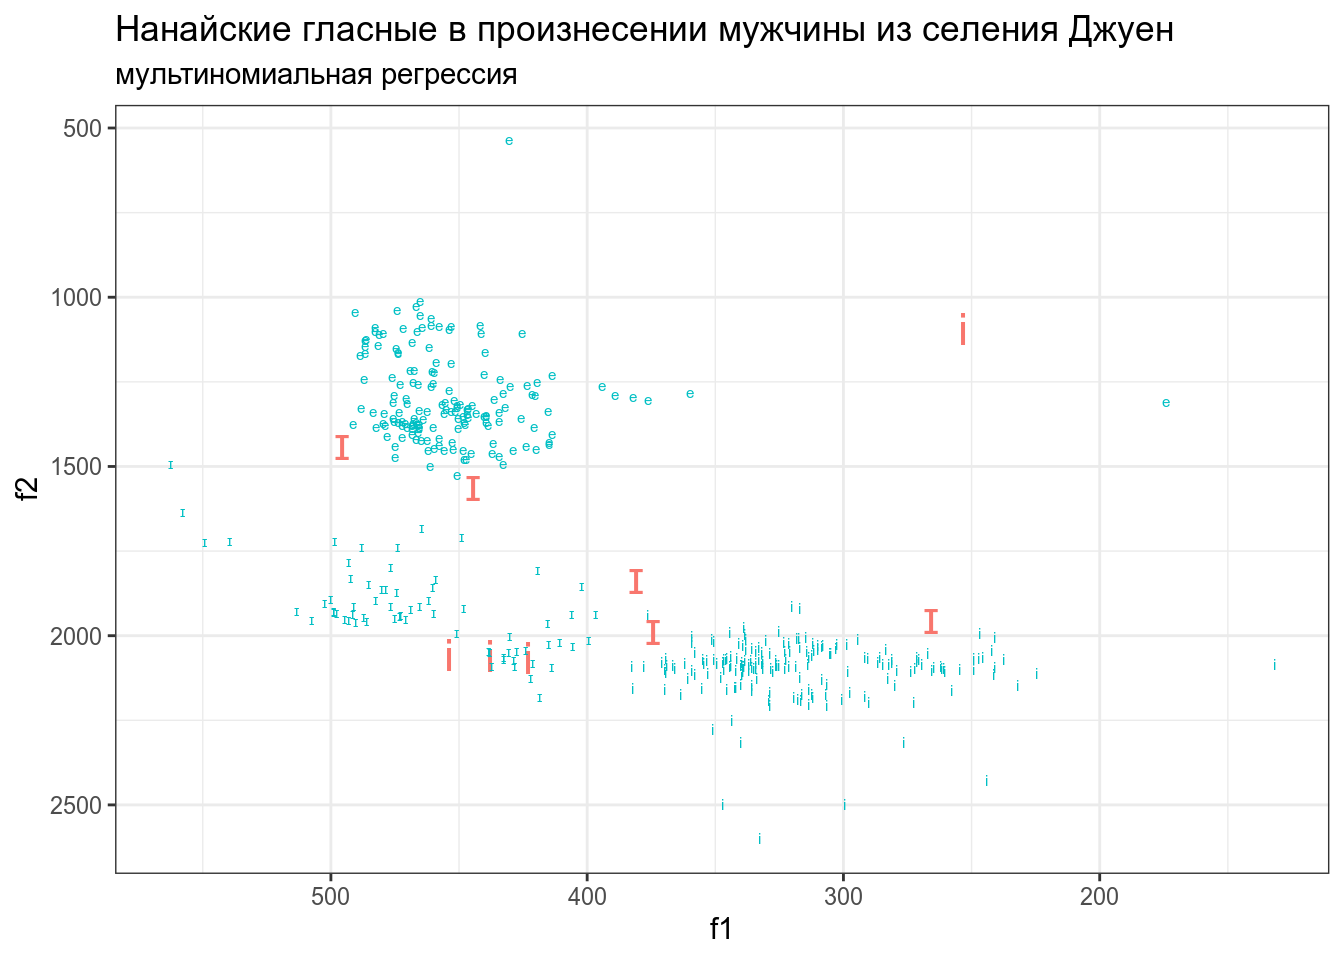
\includegraphics{da4l_files/figure-latex/unnamed-chunk-34-1.pdf}

\begin{rmdtask}
Если принять на веру, что логнормальное распределение с параметрами
\(\ln{\mu} =\) 5.587 и \(\ln{\sigma}=\) 0.242 описывает данные
длительности гласных американского английского из {[}@hillenbrand95{]},
то какова вероятность наблюдать значения между 300 и 400 мс? То же самое
можно записать, используя математическую нотацию:

\[P\left(X \in [300,\, 400] | X \sim \ln{\mathcal{N}}(\ln{\mu} = 5.587, \ln{\sigma}=0.242)\right) = ??\]
Ответ округлите до трех и меньше знаков после запятой.
\end{rmdtask}

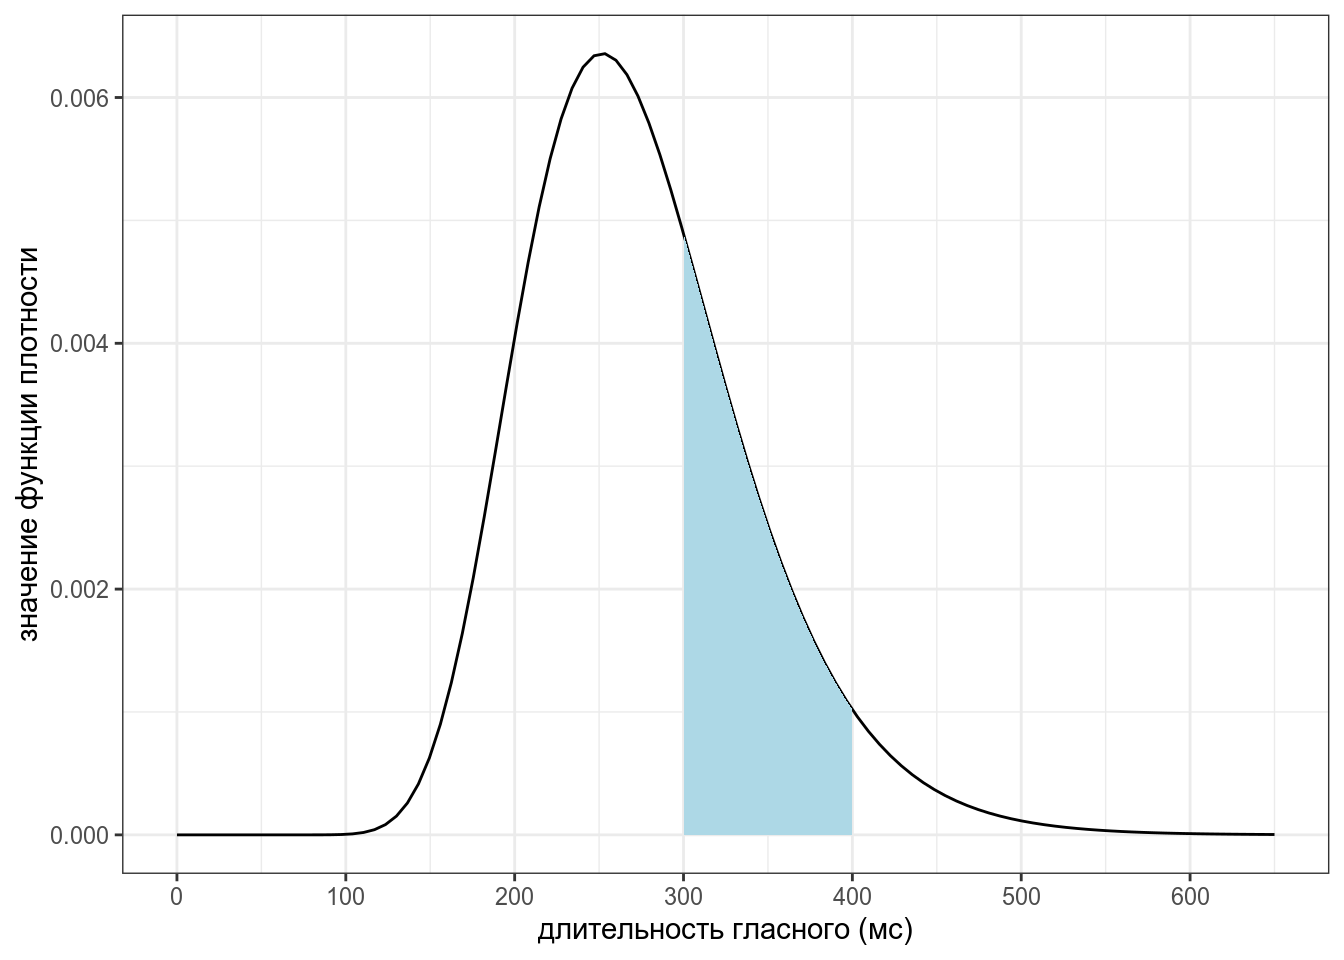
\includegraphics{da4l_files/figure-latex/unnamed-chunk-36-1.pdf}

\begin{rmdtask}
Если принять на веру, что биномиальное распределение с параметрами
\(p =\) 0.9 описывает, согласно {[}@rosenbach03: 394{]} употребление
\emph{s}-генитивов в британском английском, то какова вероятность
наблюдать значения между 300 и 350 генитивов в интервью, содержащее 400
генитивных контекстов? То же самое можно записать, используя
математическую нотацию:

\[P\left(X \in [300,\, 350] | X \sim Binom(n = 400, p = 0.9)\right) = ??\]
Ответ округлите до трех и меньше знаков после запятой.
\end{rmdtask}

\hypertarget{ux444ux443ux43dux43aux446ux438ux44f-ux43fux440ux430ux432ux434ux43eux43fux43eux434ux43eux431ux438ux44f}{%
\section{Функция правдоподобия}\label{ux444ux443ux43dux43aux446ux438ux44f-ux43fux440ux430ux432ux434ux43eux43fux43eux434ux43eux431ux438ux44f}}

Если при поиске вероятностей, мы предполагали, что данные нам \textbf{неизвестны}, а распределение и его параметры \textbf{известны}, то функция правдоподобия позволяет этот процесс перевернуть, запустив поиск параметров распределения, при изветсных данных и семье распределения:

\[L\left(X \sim Distr(...)|x\right) = ...\]

Таким образом получается, что на основании функции плотности мы можем сравнивать, какой параметр лучше подходит к нашим данным.

Для примера рассмотрим наш s-генетив: мы провели интервью и нам встретилось 85 \emph{s}-генетивов из 100 случаев всех генетивов. Насколько хорошо подходит нам распределение с параметром \emph{p} = 0.9?

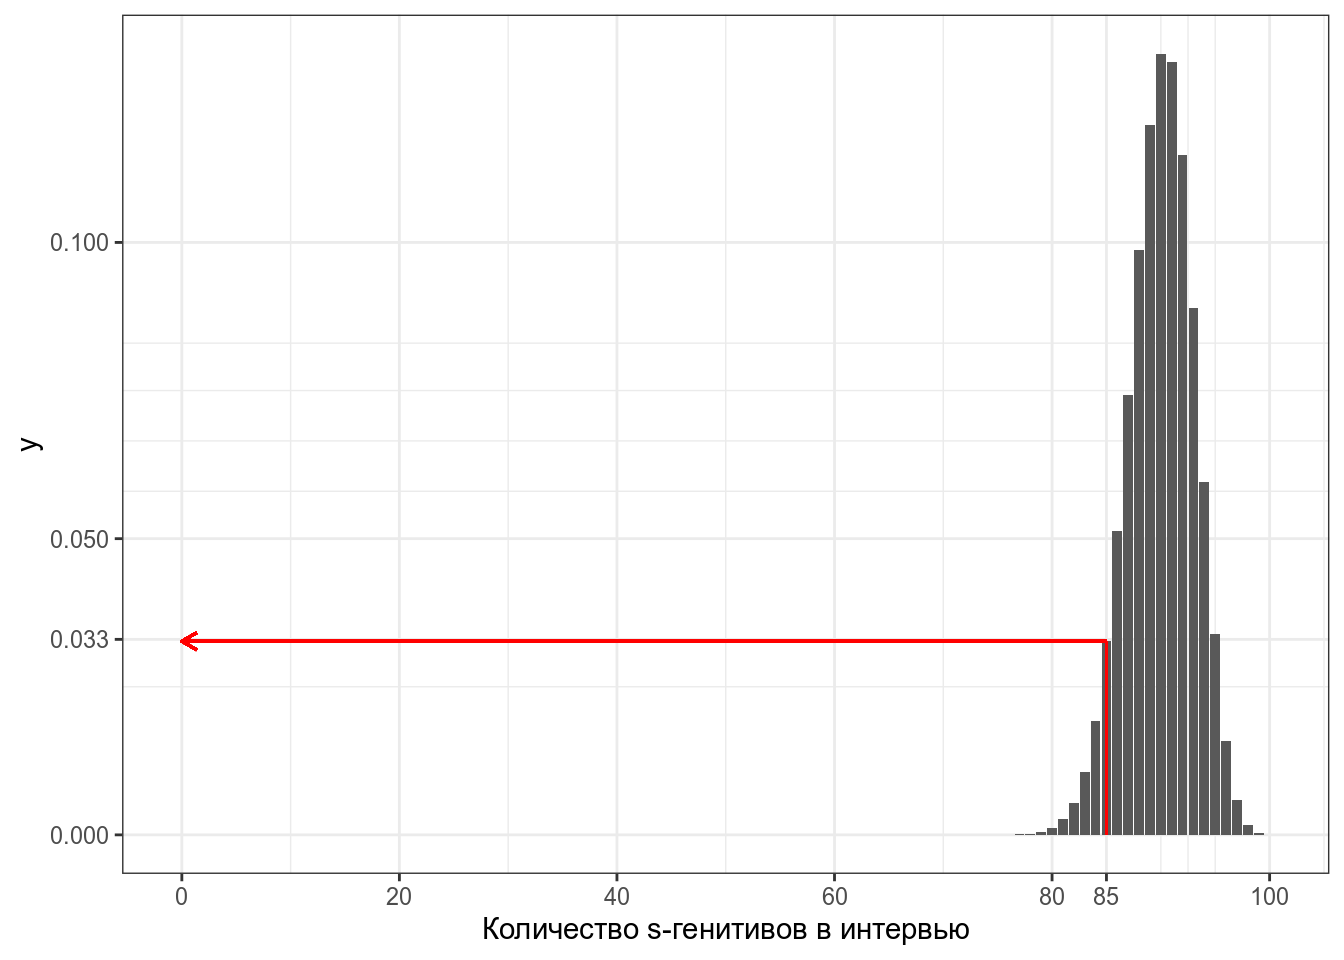
\includegraphics{da4l_files/figure-latex/unnamed-chunk-40-1.pdf}

Ответ:

\begin{Shaded}
\begin{Highlighting}[]
\FunctionTok{dbinom}\NormalTok{(}\DecValTok{85}\NormalTok{, }\DecValTok{100}\NormalTok{, }\FloatTok{0.9}\NormalTok{)}
\end{Highlighting}
\end{Shaded}

\begin{verbatim}
[1] 0.03268244
\end{verbatim}

Представим теперь это как функцию от параметра \emph{p}:

\begin{Shaded}
\begin{Highlighting}[]
\FunctionTok{tibble}\NormalTok{(}\AttributeTok{p =} \FunctionTok{seq}\NormalTok{(}\DecValTok{0}\NormalTok{, }\DecValTok{1}\NormalTok{, }\AttributeTok{by =} \FloatTok{0.01}\NormalTok{)) }\SpecialCharTok{\%\textgreater{}\%} 
  \FunctionTok{ggplot}\NormalTok{(}\FunctionTok{aes}\NormalTok{(p)) }\SpecialCharTok{+}
  \FunctionTok{stat\_function}\NormalTok{(}\AttributeTok{fun =} \ControlFlowTok{function}\NormalTok{(p) }\FunctionTok{dbinom}\NormalTok{(}\DecValTok{85}\NormalTok{, }\DecValTok{100}\NormalTok{, p), }\AttributeTok{geom =} \StringTok{"col"}\NormalTok{)}\SpecialCharTok{+}
  \FunctionTok{labs}\NormalTok{(}\AttributeTok{x =} \StringTok{"параметр биномиального распределения p"}\NormalTok{,}
       \AttributeTok{y =} \StringTok{"значение функции правдоподобия}\SpecialCharTok{\textbackslash{}n}\StringTok{(одно наблюдение)"}\NormalTok{)}
\end{Highlighting}
\end{Shaded}

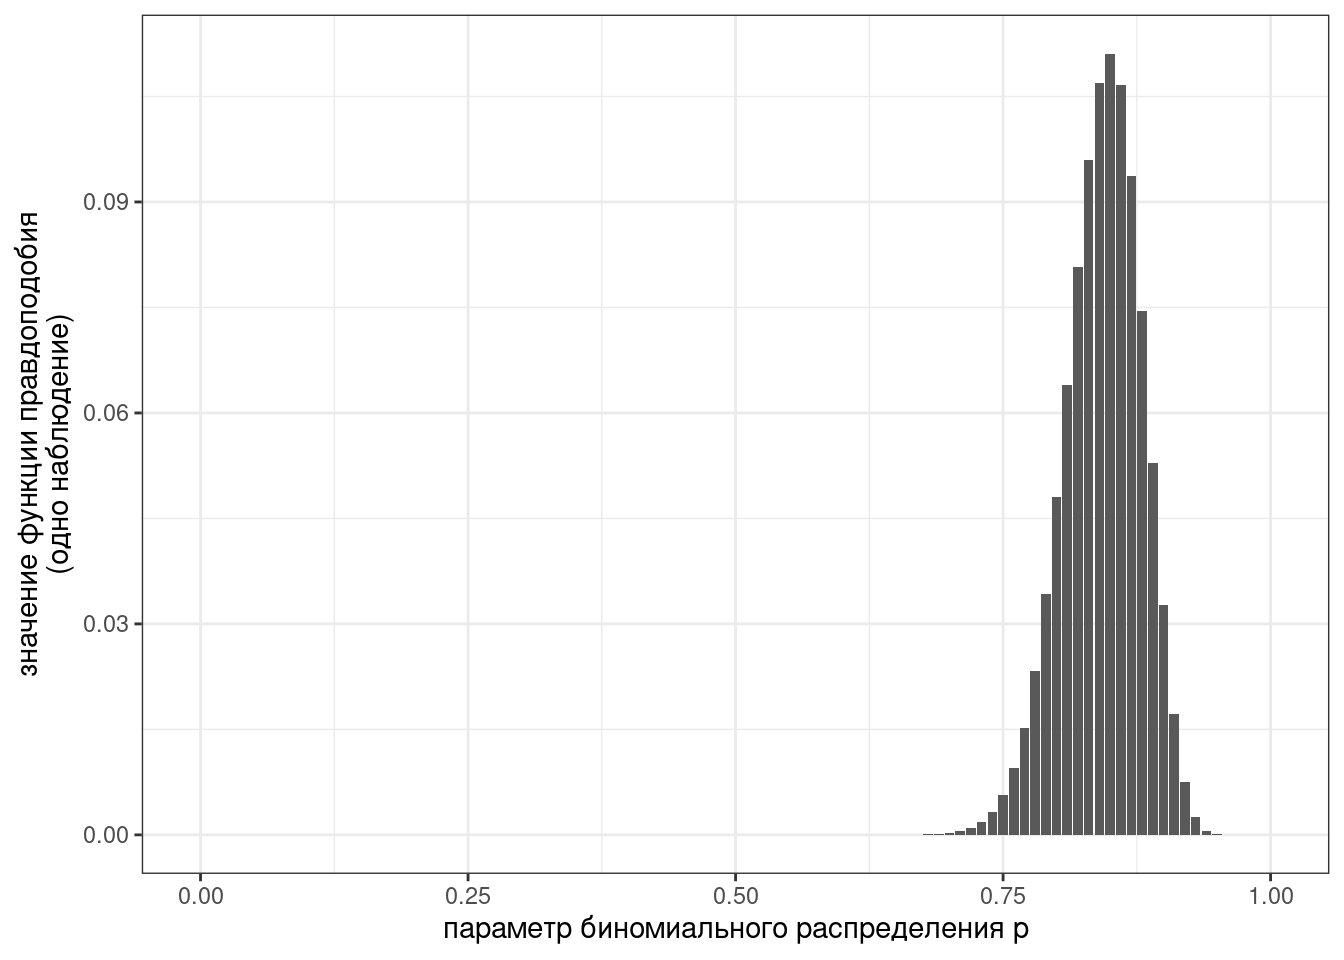
\includegraphics{da4l_files/figure-latex/unnamed-chunk-42-1.pdf}

А что если мы располагаем двумя интервью одного актера? В первом на сто генитивов пришлось 85 s-генитивов, а во втором -- 89. В таком случае, также как и с вероятностью наступления двух независимых событий, значения функции плотности перемножаются.

\begin{Shaded}
\begin{Highlighting}[]
\FunctionTok{dbinom}\NormalTok{(}\DecValTok{85}\NormalTok{, }\DecValTok{100}\NormalTok{, }\FloatTok{0.9}\NormalTok{)}\SpecialCharTok{*}\FunctionTok{dbinom}\NormalTok{(}\DecValTok{89}\NormalTok{, }\DecValTok{100}\NormalTok{, }\FloatTok{0.9}\NormalTok{)}
\end{Highlighting}
\end{Shaded}

\begin{verbatim}
[1] 0.003917892
\end{verbatim}

\begin{Shaded}
\begin{Highlighting}[]
\FunctionTok{tibble}\NormalTok{(}\AttributeTok{p =} \FunctionTok{seq}\NormalTok{(}\DecValTok{0}\NormalTok{, }\DecValTok{1}\NormalTok{, }\AttributeTok{by =} \FloatTok{0.01}\NormalTok{)) }\SpecialCharTok{\%\textgreater{}\%} 
  \FunctionTok{ggplot}\NormalTok{(}\FunctionTok{aes}\NormalTok{(p)) }\SpecialCharTok{+}
  \FunctionTok{stat\_function}\NormalTok{(}\AttributeTok{fun =} \ControlFlowTok{function}\NormalTok{(p) }\FunctionTok{dbinom}\NormalTok{(}\DecValTok{85}\NormalTok{, }\DecValTok{100}\NormalTok{, p)}\SpecialCharTok{*}\FunctionTok{dbinom}\NormalTok{(}\DecValTok{89}\NormalTok{, }\DecValTok{100}\NormalTok{, p), }\AttributeTok{geom =} \StringTok{"col"}\NormalTok{)}\SpecialCharTok{+}
  \FunctionTok{labs}\NormalTok{(}\AttributeTok{x =} \StringTok{"параметр биномиального распределения p"}\NormalTok{,}
       \AttributeTok{y =} \StringTok{"значение функции правдоподобия}\SpecialCharTok{\textbackslash{}n}\StringTok{(два наблюдения)"}\NormalTok{)}
\end{Highlighting}
\end{Shaded}

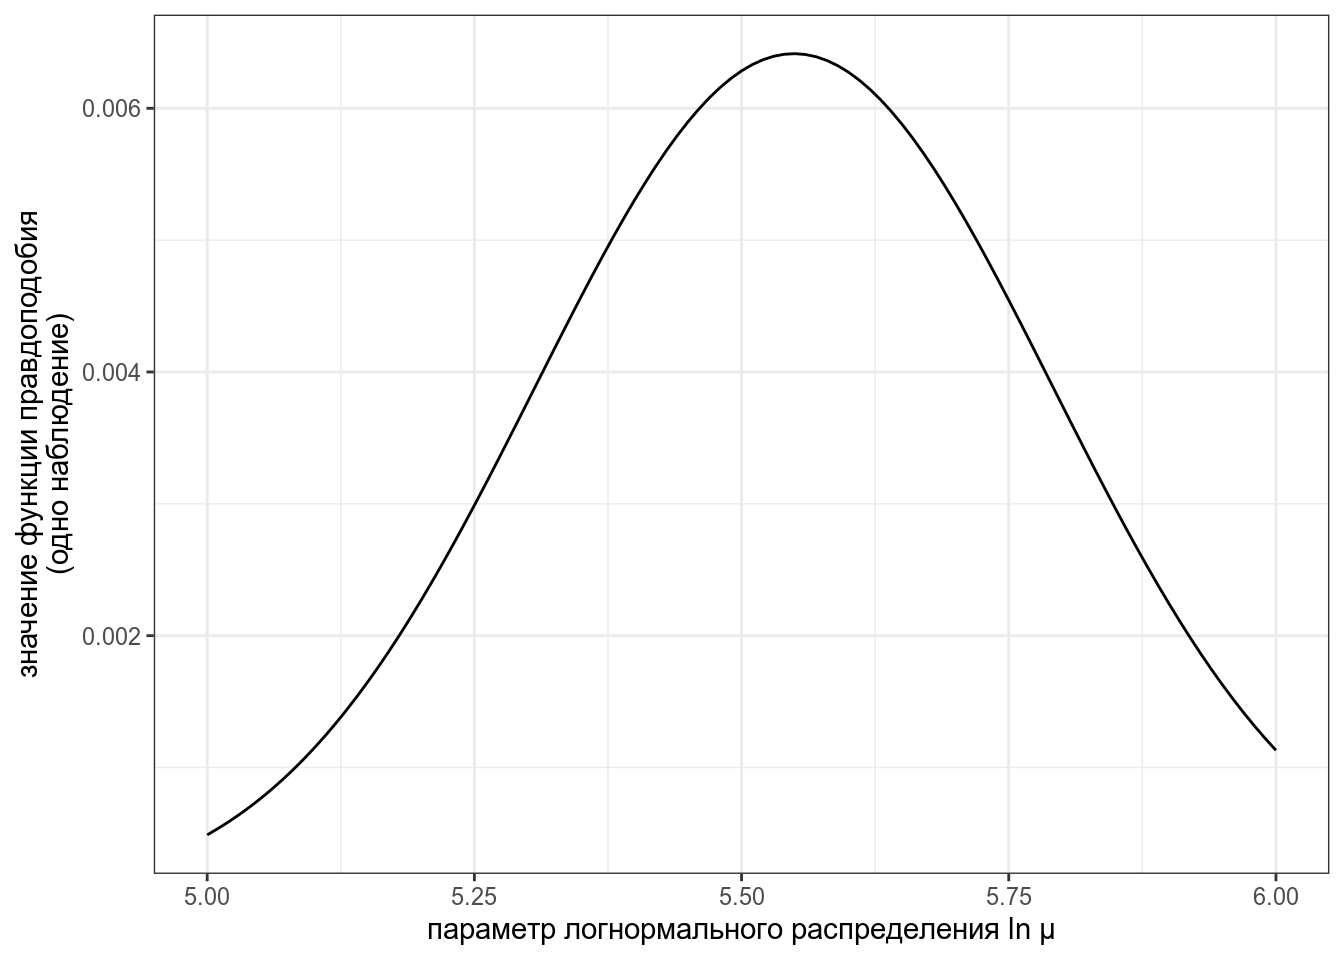
\includegraphics{da4l_files/figure-latex/unnamed-chunk-44-1.pdf}

В итоге:

\begin{itemize}
\tightlist
\item
  вероятность --- P(data\textbar distribution)
\item
  правдоподобие --- L(distribution\textbar data)
\end{itemize}

Интеграл распределения/сумма значений вероятностей равен/на 1. \href{https://stats.stackexchange.com/a/31241/225843}{Интеграл распределения/сумма значений правдоподобия может быть не равен/на 1}.

\hypertarget{ux43fux440ux438ux43cux435ux440-ux441-ux43dux435ux43fux440ux435ux440ux44bux432ux43dux44bux43c-ux440ux430ux441ux43fux440ux435ux434ux435ux43bux435ux43dux438ux435ux43c}{%
\section{Пример с непрерывным распределением}\label{ux43fux440ux438ux43cux435ux440-ux441-ux43dux435ux43fux440ux435ux440ux44bux432ux43dux44bux43c-ux440ux430ux441ux43fux440ux435ux434ux435ux43bux435ux43dux438ux435ux43c}}

Мы уже обсуждали, что длительность гласных американского английского из \citep{hillenbrand95} можно описать логнормальным распределением с параметрами \(\ln\mu\) и \(\ln\sigma\). Предположим, что \(\ln\sigma = 0.342\), построим функцию правдоподобия для \(\ln\mu\):

\begin{Shaded}
\begin{Highlighting}[]
\NormalTok{vowels }\OtherTok{\textless{}{-}} \FunctionTok{read\_csv}\NormalTok{(}\StringTok{"https://raw.githubusercontent.com/agricolamz/2021\_da4l/master/data/phonTools\_hillenbrand\_1995.csv"}\NormalTok{) }

\FunctionTok{tibble}\NormalTok{(}\AttributeTok{ln\_mu =} \FunctionTok{seq}\NormalTok{(}\DecValTok{5}\NormalTok{, }\DecValTok{6}\NormalTok{, }\AttributeTok{by =} \FloatTok{0.001}\NormalTok{)) }\SpecialCharTok{\%\textgreater{}\%} 
  \FunctionTok{ggplot}\NormalTok{(}\FunctionTok{aes}\NormalTok{(ln\_mu)) }\SpecialCharTok{+} 
  \FunctionTok{stat\_function}\NormalTok{(}\AttributeTok{fun =} \ControlFlowTok{function}\NormalTok{(ln\_mu) }\FunctionTok{dlnorm}\NormalTok{(vowels}\SpecialCharTok{$}\NormalTok{dur[}\DecValTok{1}\NormalTok{], }\AttributeTok{meanlog =}\NormalTok{ ln\_mu, }\AttributeTok{sdlog =} \FloatTok{0.242}\NormalTok{))}\SpecialCharTok{+}
  \FunctionTok{labs}\NormalTok{(}\AttributeTok{x =} \StringTok{"параметр логнормального распределения ln μ"}\NormalTok{,}
       \AttributeTok{y =} \StringTok{"значение функции правдоподобия}\SpecialCharTok{\textbackslash{}n}\StringTok{(одно наблюдение)"}\NormalTok{)}
\end{Highlighting}
\end{Shaded}

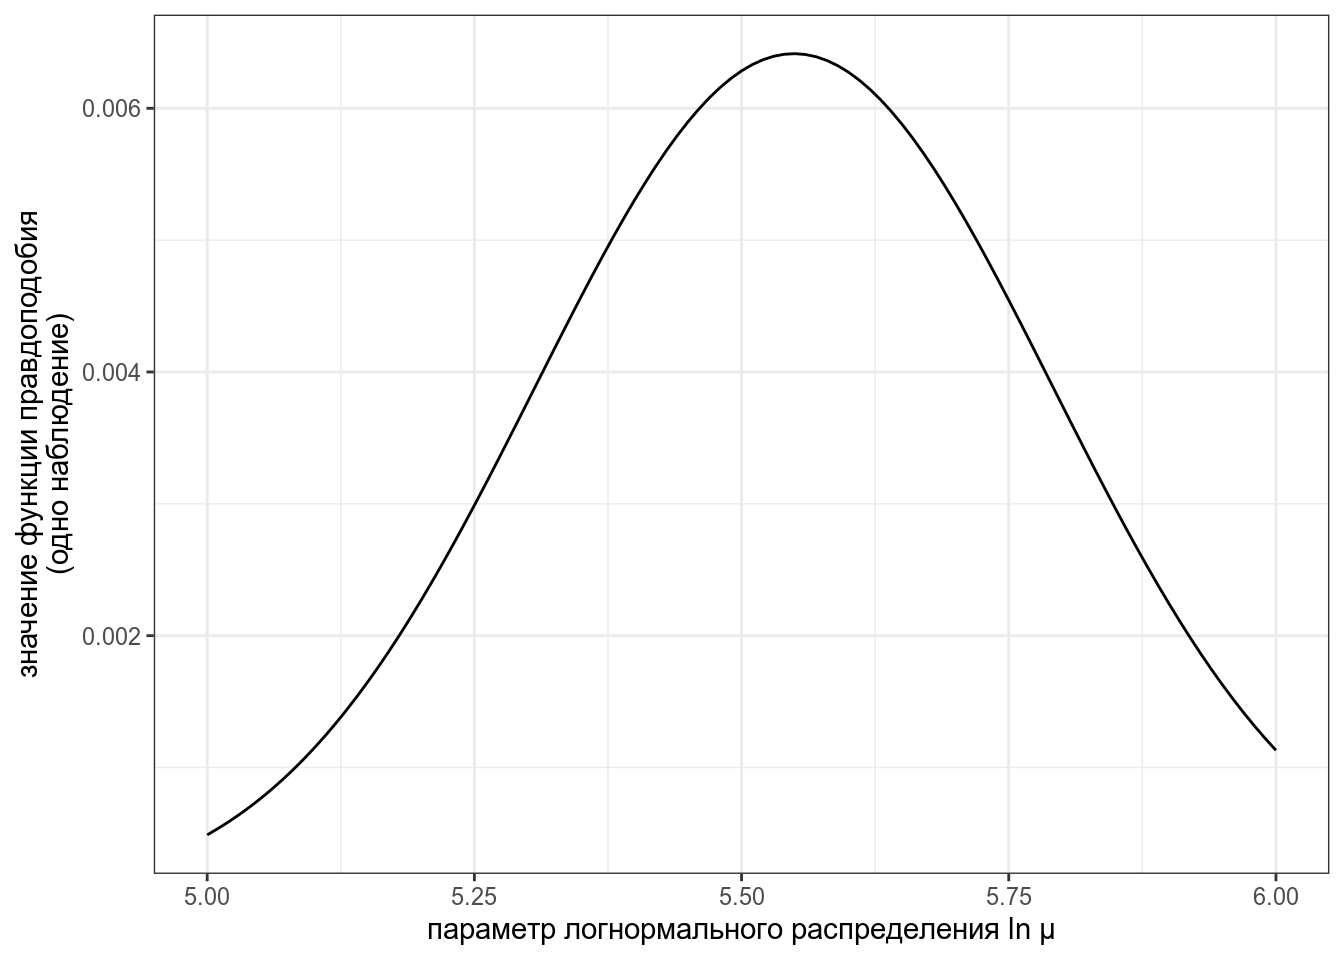
\includegraphics{da4l_files/figure-latex/unnamed-chunk-45-1.pdf}

\begin{Shaded}
\begin{Highlighting}[]
\FunctionTok{tibble}\NormalTok{(}\AttributeTok{ln\_mu =} \FunctionTok{seq}\NormalTok{(}\DecValTok{5}\NormalTok{, }\DecValTok{6}\NormalTok{, }\AttributeTok{by =} \FloatTok{0.001}\NormalTok{)) }\SpecialCharTok{\%\textgreater{}\%} 
  \FunctionTok{ggplot}\NormalTok{(}\FunctionTok{aes}\NormalTok{(ln\_mu)) }\SpecialCharTok{+} 
  \FunctionTok{stat\_function}\NormalTok{(}\AttributeTok{fun =} \ControlFlowTok{function}\NormalTok{(ln\_mu) }\FunctionTok{dlnorm}\NormalTok{(vowels}\SpecialCharTok{$}\NormalTok{dur[}\DecValTok{1}\NormalTok{], }\AttributeTok{meanlog =}\NormalTok{ ln\_mu, }\AttributeTok{sdlog =} \FloatTok{0.242}\NormalTok{)}\SpecialCharTok{*}\FunctionTok{dlnorm}\NormalTok{(vowels}\SpecialCharTok{$}\NormalTok{dur[}\DecValTok{2}\NormalTok{], }\AttributeTok{meanlog =}\NormalTok{ ln\_mu, }\AttributeTok{sdlog =} \FloatTok{0.242}\NormalTok{))}\SpecialCharTok{+}
  \FunctionTok{labs}\NormalTok{(}\AttributeTok{x =} \StringTok{"параметр логнормального распределения ln μ"}\NormalTok{,}
       \AttributeTok{y =} \StringTok{"значение функции правдоподобия}\SpecialCharTok{\textbackslash{}n}\StringTok{(два наблюдения)"}\NormalTok{)}
\end{Highlighting}
\end{Shaded}

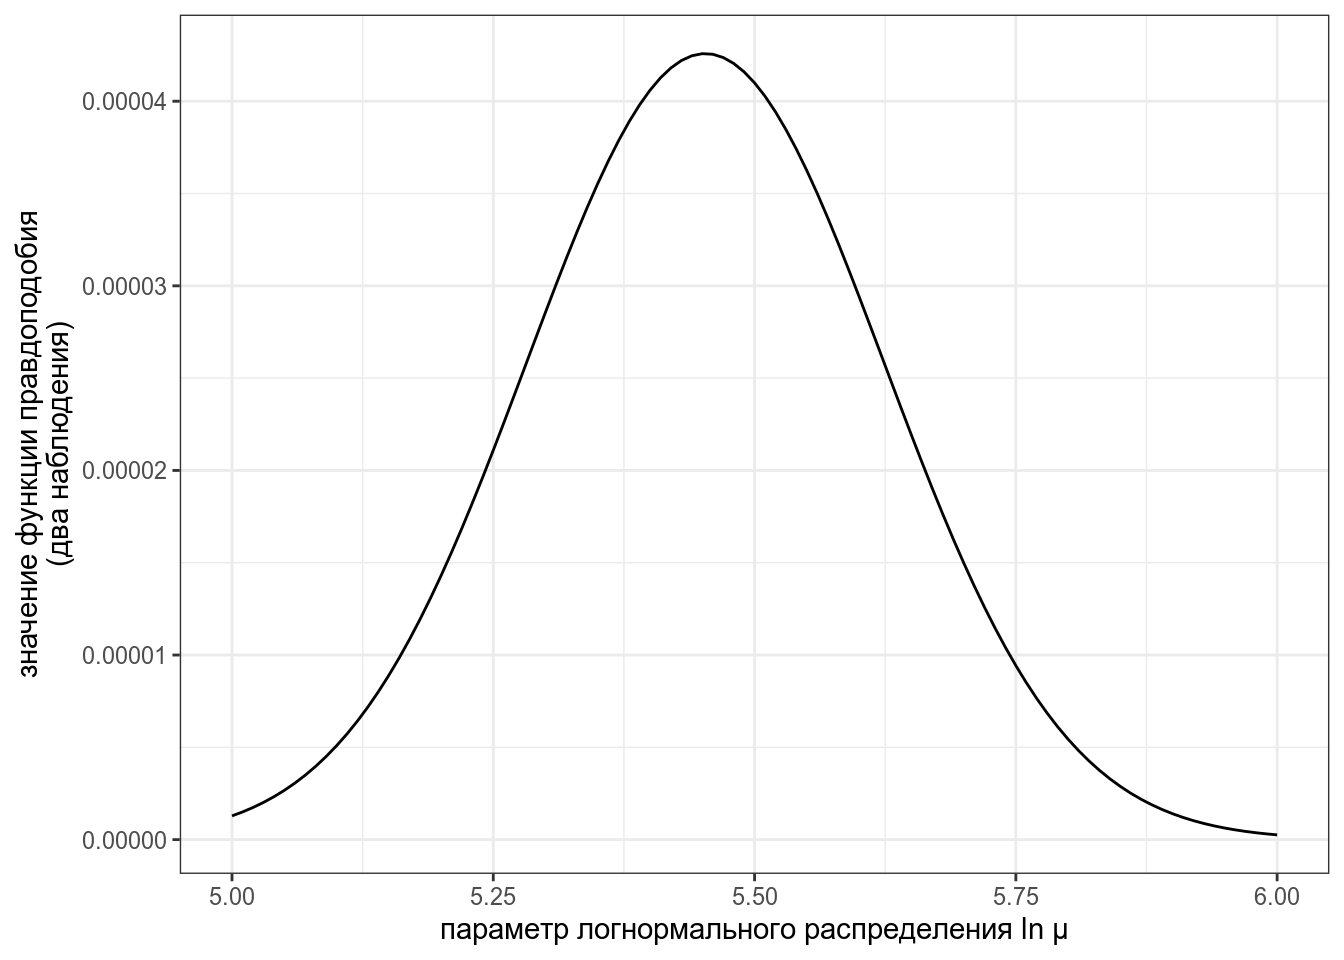
\includegraphics{da4l_files/figure-latex/unnamed-chunk-45-2.pdf}

\begin{Shaded}
\begin{Highlighting}[]
\FunctionTok{tibble}\NormalTok{(}\AttributeTok{ln\_mu =} \FunctionTok{seq}\NormalTok{(}\DecValTok{5}\NormalTok{, }\DecValTok{6}\NormalTok{, }\AttributeTok{by =} \FloatTok{0.001}\NormalTok{)) }\SpecialCharTok{\%\textgreater{}\%} 
  \FunctionTok{ggplot}\NormalTok{(}\FunctionTok{aes}\NormalTok{(ln\_mu)) }\SpecialCharTok{+} 
  \FunctionTok{stat\_function}\NormalTok{(}\AttributeTok{fun =} \ControlFlowTok{function}\NormalTok{(ln\_mu) }\FunctionTok{dlnorm}\NormalTok{(vowels}\SpecialCharTok{$}\NormalTok{dur[}\DecValTok{1}\NormalTok{], }\AttributeTok{meanlog =}\NormalTok{ ln\_mu, }\AttributeTok{sdlog =} \FloatTok{0.242}\NormalTok{)}\SpecialCharTok{*}\FunctionTok{dlnorm}\NormalTok{(vowels}\SpecialCharTok{$}\NormalTok{dur[}\DecValTok{2}\NormalTok{], }\AttributeTok{meanlog =}\NormalTok{ ln\_mu, }\AttributeTok{sdlog =} \FloatTok{0.242}\NormalTok{)}\SpecialCharTok{*}\FunctionTok{dlnorm}\NormalTok{(vowels}\SpecialCharTok{$}\NormalTok{dur[}\DecValTok{3}\NormalTok{], }\AttributeTok{meanlog =}\NormalTok{ ln\_mu, }\AttributeTok{sdlog =} \FloatTok{0.242}\NormalTok{))}\SpecialCharTok{+}
  \FunctionTok{labs}\NormalTok{(}\AttributeTok{x =} \StringTok{"параметр логнормального распределения ln μ"}\NormalTok{,}
       \AttributeTok{y =} \StringTok{"значение функции правдоподобия}\SpecialCharTok{\textbackslash{}n}\StringTok{(три наблюдения)"}\NormalTok{)}
\end{Highlighting}
\end{Shaded}

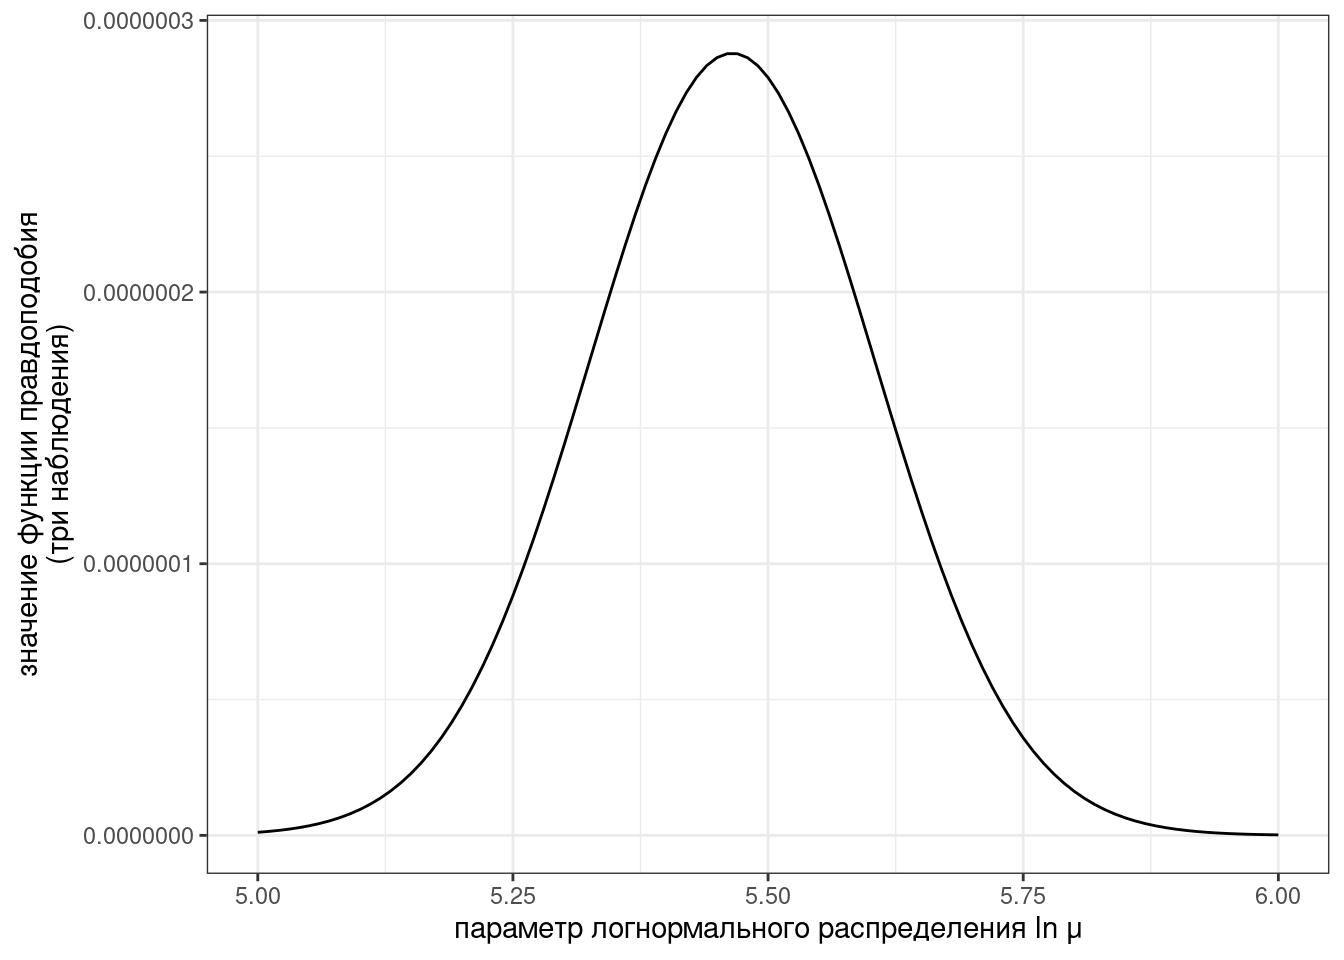
\includegraphics{da4l_files/figure-latex/unnamed-chunk-45-3.pdf}

Для простоты в начале я зафиксировал один из параметров логнормального распредления: лог стандартное отклонение. Конечно, это совсем необязательно делать: можно создать матрицу значений лог среднего и лог стандартного отклонения и получить для каждой ячейки матрицы значения функции правдоподобия.

\hypertarget{ux43cux435ux442ux43eux434-ux43cux430ux43aux441ux438ux43cux430ux43bux44cux43dux43eux433ux43e-ux43fux440ux430ux432ux434ux43eux43fux43eux434ux43eux431ux438ux44f-mle}{%
\section{Метод максимального правдоподобия (MLE)}\label{ux43cux435ux442ux43eux434-ux43cux430ux43aux441ux438ux43cux430ux43bux44cux43dux43eux433ux43e-ux43fux440ux430ux432ux434ux43eux43fux43eux434ux43eux431ux438ux44f-mle}}

Функция правдоподобия позволяет подбирать параметры распределения. Оценка параметров распределения при помощи функции максимального правдоподобия получила название метод максимального правдоподобия. Его я и использовал ранее для того, чтобы получить значения распределений для заданий из первого занятия:

\begin{itemize}
\tightlist
\item
  данные длительности американских гласных из \citep{hillenbrand95} и логнормальное распределение
\end{itemize}

\begin{Shaded}
\begin{Highlighting}[]
\FunctionTok{library}\NormalTok{(fitdistrplus)}
\FunctionTok{fitdist}\NormalTok{(vowels}\SpecialCharTok{$}\NormalTok{dur, }\AttributeTok{distr =} \StringTok{\textquotesingle{}lnorm\textquotesingle{}}\NormalTok{, }\AttributeTok{method =} \StringTok{\textquotesingle{}mle\textquotesingle{}}\NormalTok{)}
\end{Highlighting}
\end{Shaded}

\begin{verbatim}
Fitting of the distribution ' lnorm ' by maximum likelihood 
Parameters:
         estimate  Std. Error
meanlog 5.5870359 0.005935135
sdlog   0.2423978 0.004196453
\end{verbatim}

\begin{itemize}
\tightlist
\item
  количество андийских слогов в словах и распределение Пуассона
\end{itemize}

\begin{Shaded}
\begin{Highlighting}[]
\NormalTok{andic\_syllables }\OtherTok{\textless{}{-}} \FunctionTok{read\_csv}\NormalTok{(}\StringTok{"https://raw.githubusercontent.com/agricolamz/2021\_da4l/master/data/andic\_syllables.csv"}\NormalTok{) }

\NormalTok{andic\_syllables }\SpecialCharTok{\%\textgreater{}\%} 
  \FunctionTok{filter}\NormalTok{(language }\SpecialCharTok{==} \StringTok{"Andi"}\NormalTok{) }\SpecialCharTok{\%\textgreater{}\%} 
  \FunctionTok{uncount}\NormalTok{(count) }\SpecialCharTok{\%\textgreater{}\%} 
  \FunctionTok{pull}\NormalTok{(n\_syllables) }\SpecialCharTok{\%\textgreater{}\%} 
  \FunctionTok{fitdist}\NormalTok{(}\AttributeTok{distr =} \StringTok{\textquotesingle{}pois\textquotesingle{}}\NormalTok{, }\AttributeTok{method =} \StringTok{\textquotesingle{}mle\textquotesingle{}}\NormalTok{)}
\end{Highlighting}
\end{Shaded}

\begin{verbatim}
Fitting of the distribution ' pois ' by maximum likelihood 
Parameters:
       estimate Std. Error
lambda 2.782715 0.02128182
\end{verbatim}

\begin{itemize}
\tightlist
\item
  Есть и другие методы оценки параметров.
\item
  Метод максимального правдоподобия может быть чувствителен к размеру выборки.
\end{itemize}

\begin{rmdtask}
Отфильтруйте из
\href{https://raw.githubusercontent.com/agricolamz/2021_da4l/master/data/andic_syllables.csv}{данных
с количеством слогов в андийских языках} багвалинский и, используя метод
максимального правдоподобия, оцените для них параметры модели Пуассона.
\end{rmdtask}

\begin{rmdtask}
В работе {[}@coretta2016{]} собраны
\href{https://raw.githubusercontent.com/agricolamz/2021_da4l/master/data/Coretta_2017_icelandic.csv}{данные}
длительности исландских гласных. Отфильтруйте данные, оставив
односложные слова (переменная \texttt{syllables}) после придыхательного
(переменная \texttt{aspiration}), произнесенные носителем \texttt{tt01}
(переменная \texttt{speaker}) и постройте следующий график, моделируя
длительность гласных (переменная \texttt{vowel.dur}) нормальным и
логнормальным распределением. Как вам кажется, какое распределение лучше
подходит к данным? Докажите ваше утверждение, сравнив значения
правдоподобия.
\end{rmdtask}

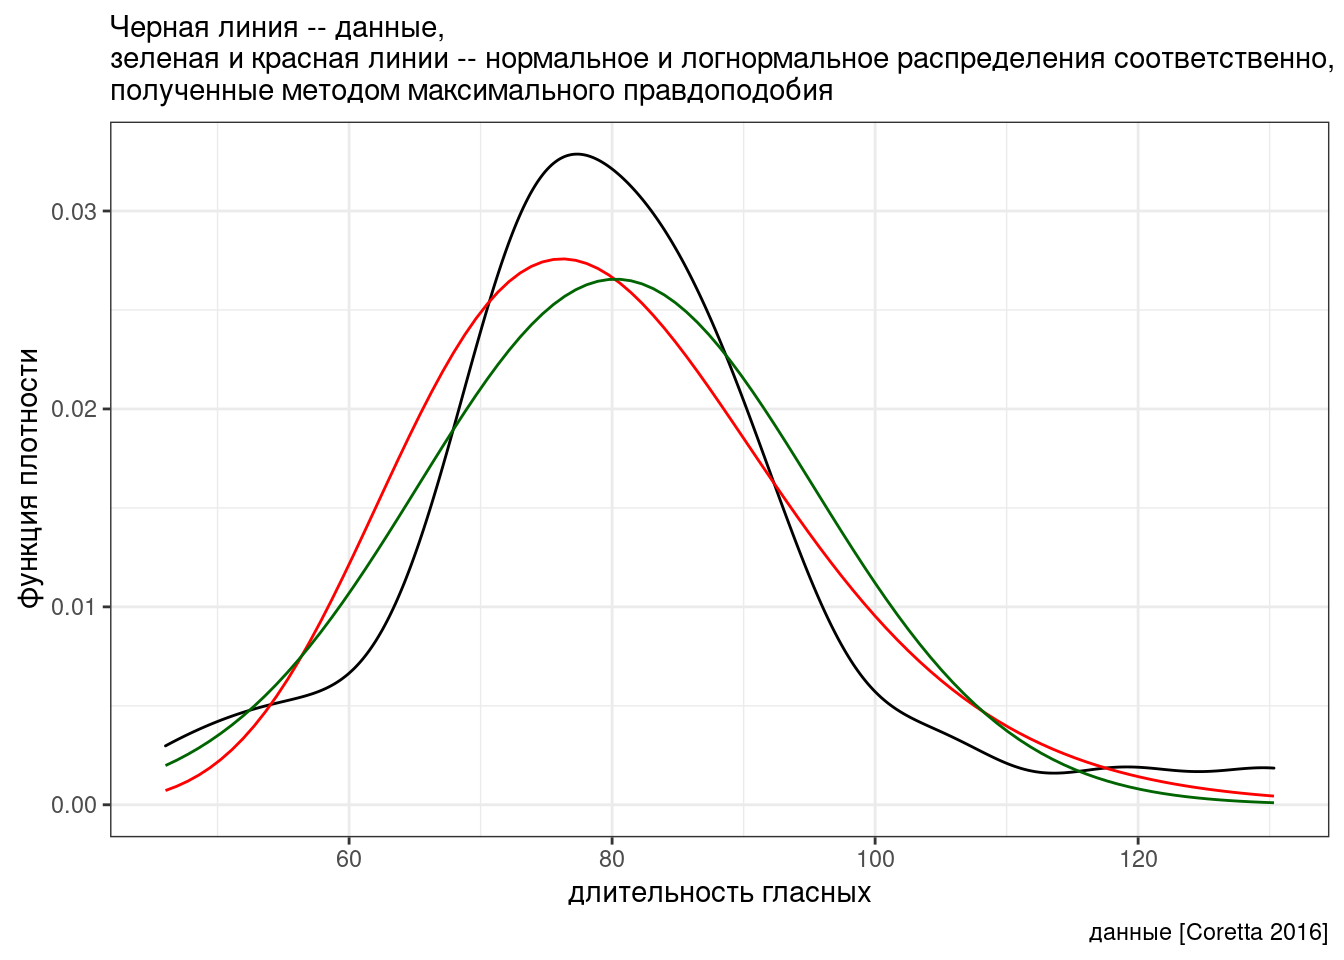
\includegraphics{da4l_files/figure-latex/unnamed-chunk-50-1.pdf}

\hypertarget{ux43bux43eux433ux43eux440ux438ux444ux43c-ux444ux443ux43dux43aux446ux438ux438-ux43fux440ux430ux432ux434ux43eux43fux43eux434ux43eux431ux438ux44f}{%
\section{Логорифм функции правдоподобия}\label{ux43bux43eux433ux43eux440ux438ux444ux43c-ux444ux443ux43dux43aux446ux438ux438-ux43fux440ux430ux432ux434ux43eux43fux43eux434ux43eux431ux438ux44f}}

Так как в большинстве случаев нужно найти лишь максимум функции правдоподобия, а не саму функцию \(\ell(x|\theta)\), то для облегчения подсчетов используют логорифмическую функцию правдоподобия \(\ln\ell(x|\theta)\): в результате, вместо произведения появляется сумма\footnote{Это просто свойство логарифмов: \texttt{log(5*5)\ =\ log(5)+log(5)}}:

\[\text{argmax}_\theta \prod \ell(\theta|x) = \text{argmax}_\theta \sum \ln\ell(\theta|x) \]

Во всех предыдущих примерах мы смотрели на 1-3 примера данных, давайте попробуем использовать функцию правдоподобия для большего набора данных.

\begin{rmdtask}
Представим, что мы проводим некоторый эксперимент, и у некоторых
участников все получается с первой попытки, а некоторым нужна еще одна
попытка или даже две. Дополните код функциями правдоподобия и
логорифмической функцией правдоподобия, чтобы получился график ниже.
\end{rmdtask}

\begin{Shaded}
\begin{Highlighting}[]
\FunctionTok{set.seed}\NormalTok{(}\DecValTok{42}\NormalTok{)}
\NormalTok{v }\OtherTok{\textless{}{-}} \FunctionTok{sample}\NormalTok{(}\DecValTok{0}\SpecialCharTok{:}\DecValTok{2}\NormalTok{, }\DecValTok{10}\NormalTok{, }\AttributeTok{replace =} \ConstantTok{TRUE}\NormalTok{)}

\FunctionTok{sapply}\NormalTok{(}\FunctionTok{seq}\NormalTok{(}\FloatTok{0.01}\NormalTok{, }\FloatTok{0.99}\NormalTok{, }\FloatTok{0.01}\NormalTok{), }\ControlFlowTok{function}\NormalTok{(p)\{}
\NormalTok{  ...}
\NormalTok{\}) }\OtherTok{{-}\textgreater{}}
\NormalTok{  likelihood}

\FunctionTok{sapply}\NormalTok{(}\FunctionTok{seq}\NormalTok{(}\FloatTok{0.01}\NormalTok{, }\FloatTok{0.99}\NormalTok{, }\FloatTok{0.01}\NormalTok{), }\ControlFlowTok{function}\NormalTok{(p)\{}
\NormalTok{  ...}
\NormalTok{\}) }\OtherTok{{-}\textgreater{}}
\NormalTok{  loglikelihood}

\FunctionTok{tibble}\NormalTok{(}\AttributeTok{p =} \FunctionTok{seq}\NormalTok{(}\FloatTok{0.01}\NormalTok{, }\FloatTok{0.99}\NormalTok{, }\FloatTok{0.01}\NormalTok{),}
\NormalTok{       loglikelihood,}
\NormalTok{       likelihood) }\SpecialCharTok{\%\textgreater{}\%} 
  \FunctionTok{pivot\_longer}\NormalTok{(}\AttributeTok{names\_to =} \StringTok{"type"}\NormalTok{, }\AttributeTok{values\_to =} \StringTok{"value"}\NormalTok{, loglikelihood}\SpecialCharTok{:}\NormalTok{likelihood) }\SpecialCharTok{\%\textgreater{}\%} 
  \FunctionTok{ggplot}\NormalTok{(}\FunctionTok{aes}\NormalTok{(p, value))}\SpecialCharTok{+}
  \FunctionTok{geom\_line}\NormalTok{()}\SpecialCharTok{+}
  \FunctionTok{geom\_vline}\NormalTok{(}\AttributeTok{xintercept =} \FloatTok{0.33}\NormalTok{, }\AttributeTok{linetype =} \DecValTok{2}\NormalTok{)}\SpecialCharTok{+}
  \FunctionTok{facet\_wrap}\NormalTok{(}\SpecialCharTok{\textasciitilde{}}\NormalTok{type, }\AttributeTok{scales =} \StringTok{"free\_y"}\NormalTok{, }\AttributeTok{nrow =} \DecValTok{2}\NormalTok{)}\SpecialCharTok{+}
  \FunctionTok{scale\_x\_continuous}\NormalTok{(}\AttributeTok{breaks =} \FunctionTok{c}\NormalTok{(}\DecValTok{0}\SpecialCharTok{:}\DecValTok{5}\SpecialCharTok{*}\FloatTok{0.25}\NormalTok{, }\FloatTok{0.33}\NormalTok{))}
\end{Highlighting}
\end{Shaded}

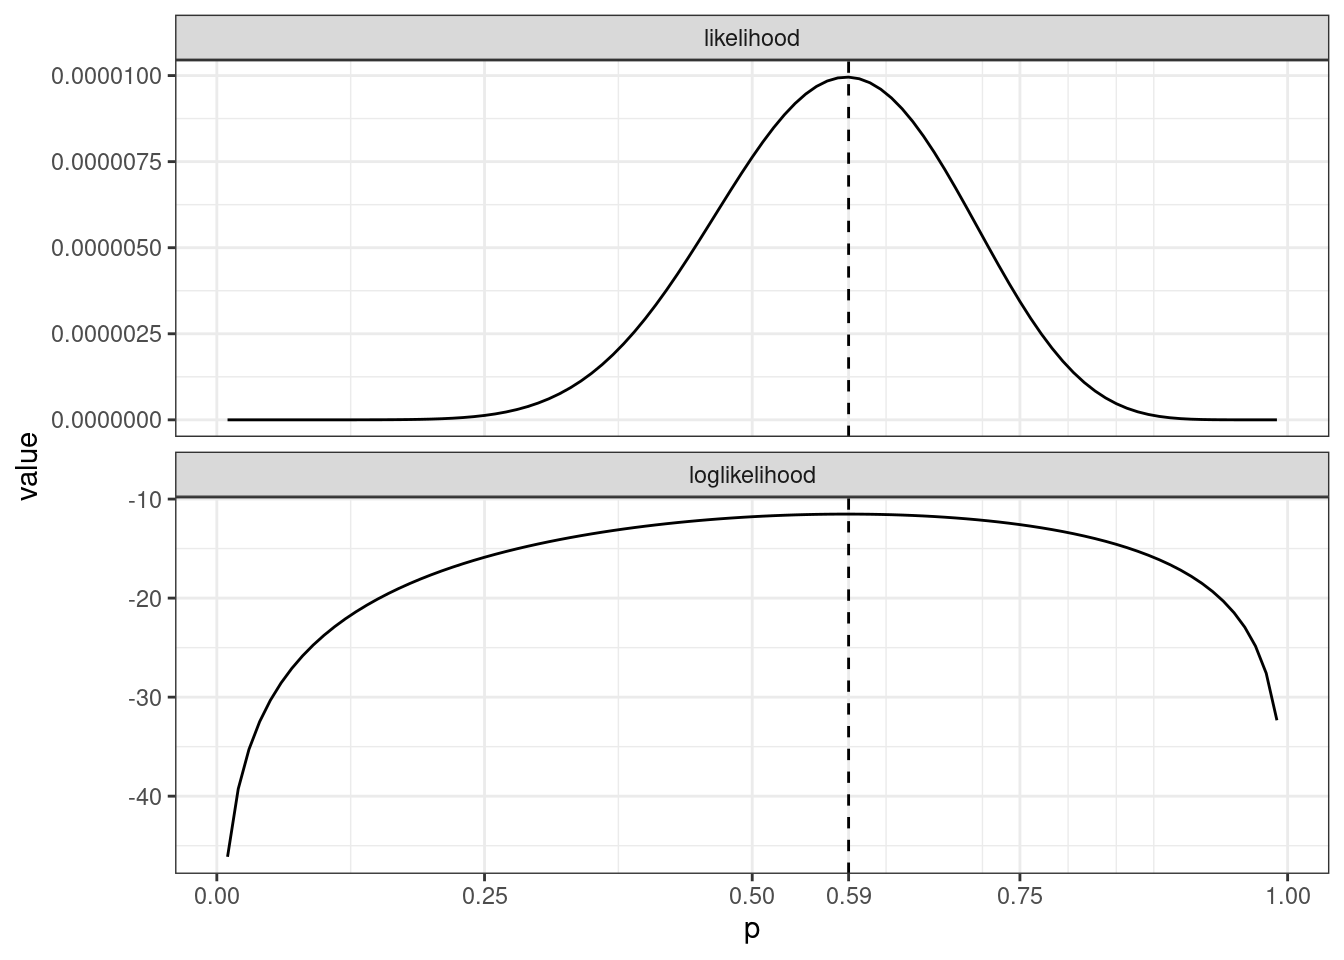
\includegraphics{da4l_files/figure-latex/unnamed-chunk-53-1.pdf}

\hypertarget{ux43cux43eux434ux435ux43bux438-ux441ux43cux435ux441ux438-ux440ux430ux441ux43fux440ux435ux434ux435ux43bux435ux43dux438ux439}{%
\chapter{Модели смеси распределений}\label{ux43cux43eux434ux435ux43bux438-ux441ux43cux435ux441ux438-ux440ux430ux441ux43fux440ux435ux434ux435ux43bux435ux43dux438ux439}}

\hypertarget{cux43cux435ux441ux438-ux440ux430ux441ux43fux440ux435ux434ux435ux43bux435ux43dux438ux439}{%
\section{Cмеси распределений}\label{cux43cux435ux441ux438-ux440ux430ux441ux43fux440ux435ux434ux435ux43bux435ux43dux438ux439}}

Не все переменные выглядят так же красиво, как распределения из учебников статистики. Для примера возьмем датасет, который содержит спамерские и обычные смс-сообщения, выложенный UCI Machine Learning \href{https://www.kaggle.com/uciml/sms-spam-collection-dataset}{на kaggle}. Посчитаем количество символов в сообщениях:

\begin{Shaded}
\begin{Highlighting}[]
\NormalTok{spam\_sms }\OtherTok{\textless{}{-}} \FunctionTok{read\_csv}\NormalTok{(}\StringTok{"https://raw.githubusercontent.com/agricolamz/2021\_da4l/master/data/spam\_sms.csv"}\NormalTok{)}

\FunctionTok{glimpse}\NormalTok{(spam\_sms)}
\end{Highlighting}
\end{Shaded}

\begin{verbatim}
Rows: 5,572
Columns: 2
$ type    <chr> "ham", "ham", "spam", "ham", "ham", "spam", "ham", "ham", "...
$ message <chr> "Go until jurong point, crazy.. Available only in bugis n g...
\end{verbatim}

\begin{Shaded}
\begin{Highlighting}[]
\NormalTok{spam\_sms }\SpecialCharTok{\%\textgreater{}\%} 
  \FunctionTok{mutate}\NormalTok{(}\AttributeTok{n\_char =} \FunctionTok{nchar}\NormalTok{(message)) }\OtherTok{{-}\textgreater{}}
\NormalTok{  spam\_sms}
  
\FunctionTok{glimpse}\NormalTok{(spam\_sms)}
\end{Highlighting}
\end{Shaded}

\begin{verbatim}
Rows: 5,572
Columns: 3
$ type    <chr> "ham", "ham", "spam", "ham", "ham", "spam", "ham", "ham", "...
$ message <chr> "Go until jurong point, crazy.. Available only in bugis n g...
$ n_char  <int> 111, 29, 155, 49, 61, 147, 77, 160, 157, 154, 109, 136, 155...
\end{verbatim}

\begin{Shaded}
\begin{Highlighting}[]
\NormalTok{spam\_sms }\SpecialCharTok{\%\textgreater{}\%} 
  \FunctionTok{ggplot}\NormalTok{(}\FunctionTok{aes}\NormalTok{(n\_char))}\SpecialCharTok{+}
  \FunctionTok{geom\_histogram}\NormalTok{(}\AttributeTok{fill =} \StringTok{"gray90"}\NormalTok{)}\SpecialCharTok{+}
  \FunctionTok{labs}\NormalTok{(}\AttributeTok{caption =} \StringTok{"данные из kaggle.com/uciml/sms{-}spam{-}collection{-}dataset"}\NormalTok{,}
       \AttributeTok{x =} \StringTok{"количество символов"}\NormalTok{,}
       \AttributeTok{y =} \StringTok{"значение функции плотности"}\NormalTok{)}
\end{Highlighting}
\end{Shaded}

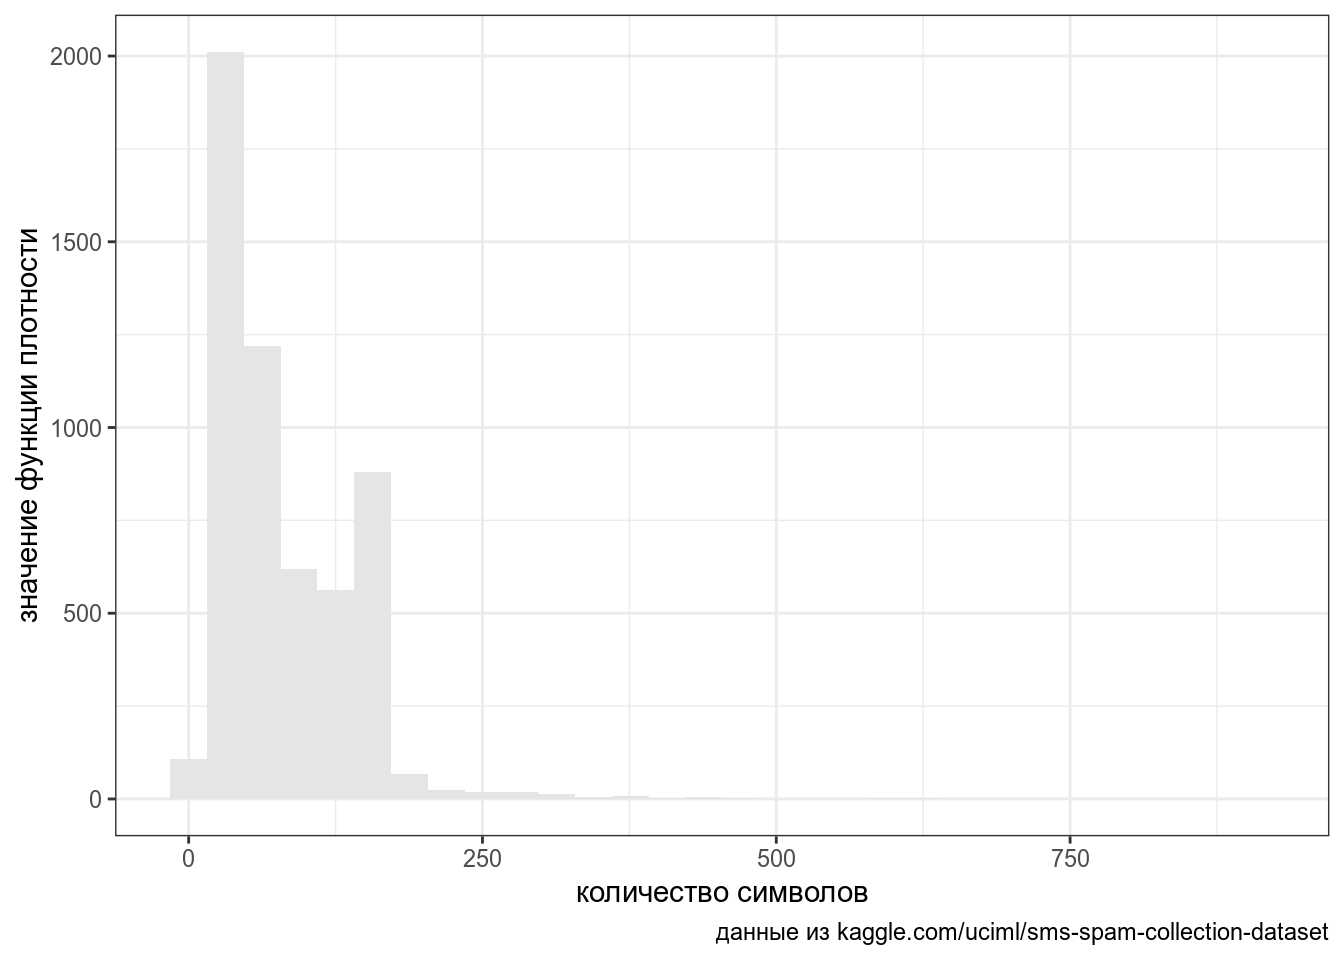
\includegraphics{da4l_files/figure-latex/unnamed-chunk-55-1.pdf}

Мы видим два явных горба и, как можно догадаться, это связано с тем, что спамерские сообщения в среднем длиннее и сосредоточены вокруг ограничения смс в 160 символов:

\begin{Shaded}
\begin{Highlighting}[]
\NormalTok{spam\_sms }\SpecialCharTok{\%\textgreater{}\%} 
  \FunctionTok{ggplot}\NormalTok{(}\FunctionTok{aes}\NormalTok{(n\_char))}\SpecialCharTok{+}
  \FunctionTok{geom\_histogram}\NormalTok{(}\AttributeTok{fill =} \StringTok{"gray70"}\NormalTok{, }\FunctionTok{aes}\NormalTok{(}\AttributeTok{y =}\NormalTok{ ..density..))}\SpecialCharTok{+}
  \FunctionTok{geom\_density}\NormalTok{(}\FunctionTok{aes}\NormalTok{(}\AttributeTok{fill =}\NormalTok{ type), }\AttributeTok{alpha =} \FloatTok{0.3}\NormalTok{)}\SpecialCharTok{+}
  \FunctionTok{labs}\NormalTok{(}\AttributeTok{caption =} \StringTok{"данные из kaggle.com/uciml/sms{-}spam{-}collection{-}dataset"}\NormalTok{,}
       \AttributeTok{x =} \StringTok{"количество символов"}\NormalTok{,}
       \AttributeTok{y =} \StringTok{"значение функции плотности"}\NormalTok{)}\SpecialCharTok{+}
  \FunctionTok{geom\_vline}\NormalTok{(}\AttributeTok{xintercept =} \DecValTok{160}\NormalTok{, }\AttributeTok{linetype =} \DecValTok{2}\NormalTok{, }\AttributeTok{size =} \FloatTok{0.3}\NormalTok{)}
\end{Highlighting}
\end{Shaded}

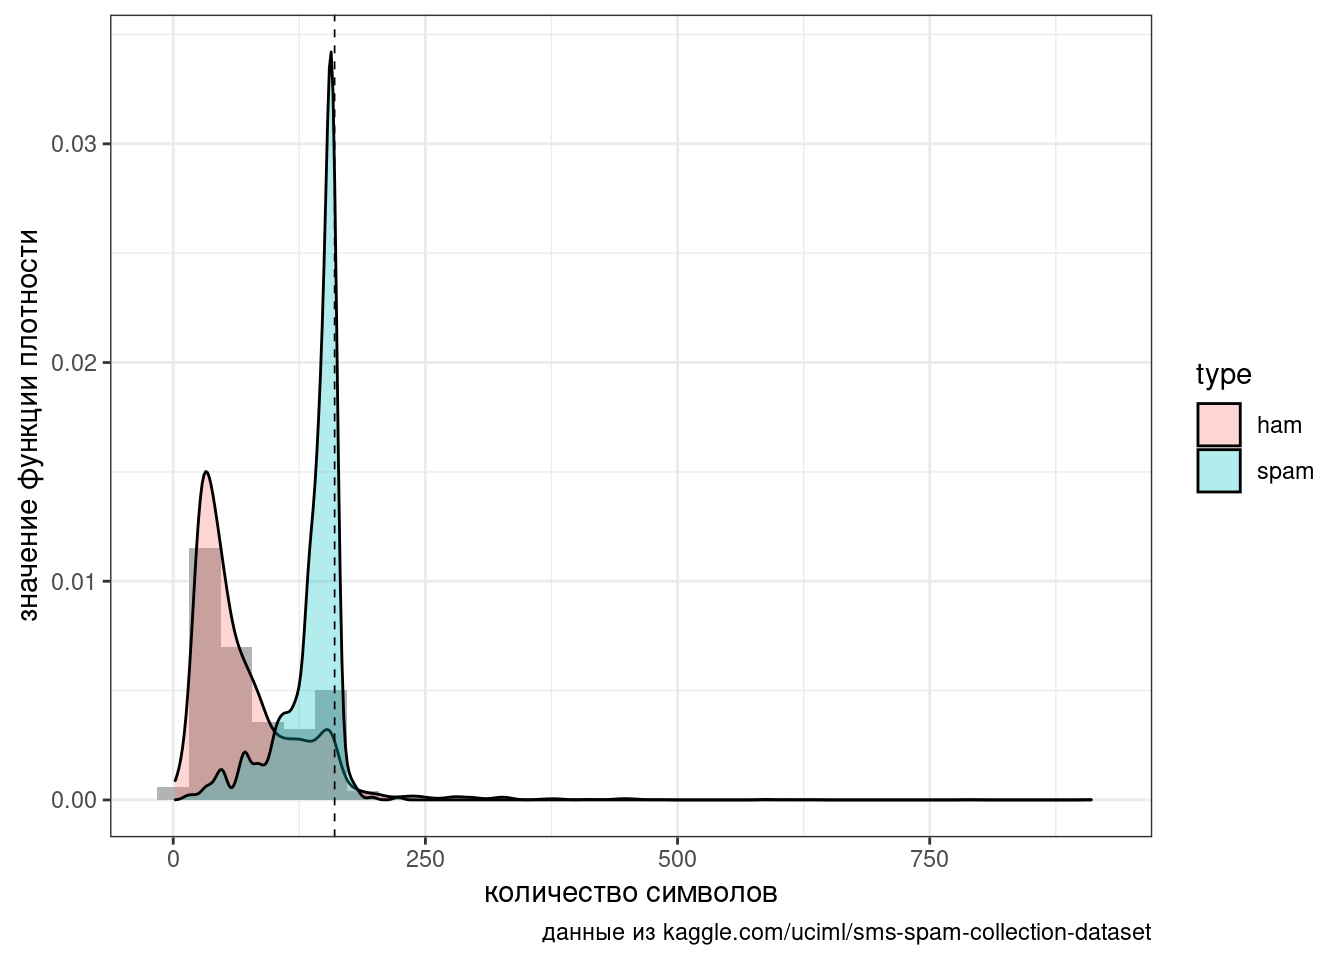
\includegraphics{da4l_files/figure-latex/unnamed-chunk-56-1.pdf}

\hypertarget{ux43cux43eux434ux435ux43bux438-ux441ux43cux435ux441ux438-ux440ux430ux441ux43fux440ux435ux434ux435ux43bux435ux43dux438ux439-1}{%
\section{Модели смеси распределений}\label{ux43cux43eux434ux435ux43bux438-ux441ux43cux435ux441ux438-ux440ux430ux441ux43fux440ux435ux434ux435ux43bux435ux43dux438ux439-1}}

Такого рода данные можно описать при помощи модели смеси разных распределений. Мы сейчас опишем нормальными распределениями, но, ясно, что семейство распределений можно было бы подобрать и получше.

\begin{Shaded}
\begin{Highlighting}[]
\FunctionTok{library}\NormalTok{(mixtools)}

\FunctionTok{set.seed}\NormalTok{(}\DecValTok{42}\NormalTok{)}
\NormalTok{spam\_length\_est }\OtherTok{\textless{}{-}} \FunctionTok{normalmixEM}\NormalTok{(spam\_sms}\SpecialCharTok{$}\NormalTok{n\_char)}
\end{Highlighting}
\end{Shaded}

\begin{verbatim}
number of iterations= 73 
\end{verbatim}

\begin{Shaded}
\begin{Highlighting}[]
\FunctionTok{summary}\NormalTok{(spam\_length\_est)}
\end{Highlighting}
\end{Shaded}

\begin{verbatim}
summary of normalmixEM object:
          comp 1     comp 2
lambda  0.439334   0.560666
mu     37.858905 114.070490
sigma  13.398985  60.921536
loglik at estimate:  -29421.36 
\end{verbatim}

Класс, получаемый в результате работы функции \texttt{normalmixEM()} имеет встроеный график:

\begin{Shaded}
\begin{Highlighting}[]
\FunctionTok{plot}\NormalTok{(spam\_length\_est, }\AttributeTok{density =} \ConstantTok{TRUE}\NormalTok{)}
\end{Highlighting}
\end{Shaded}

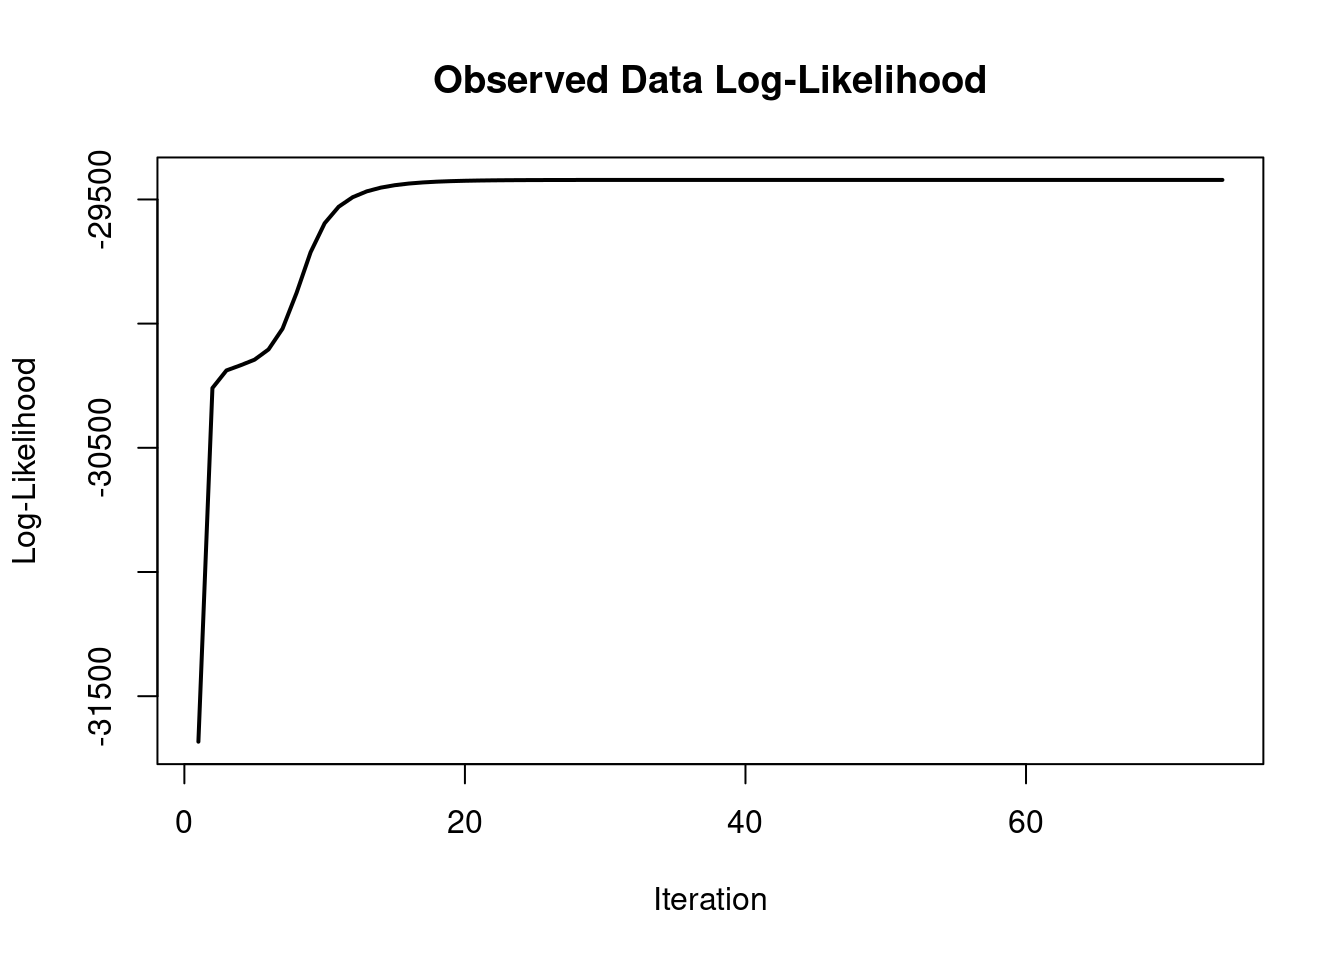
\includegraphics{da4l_files/figure-latex/unnamed-chunk-58-1.pdf} 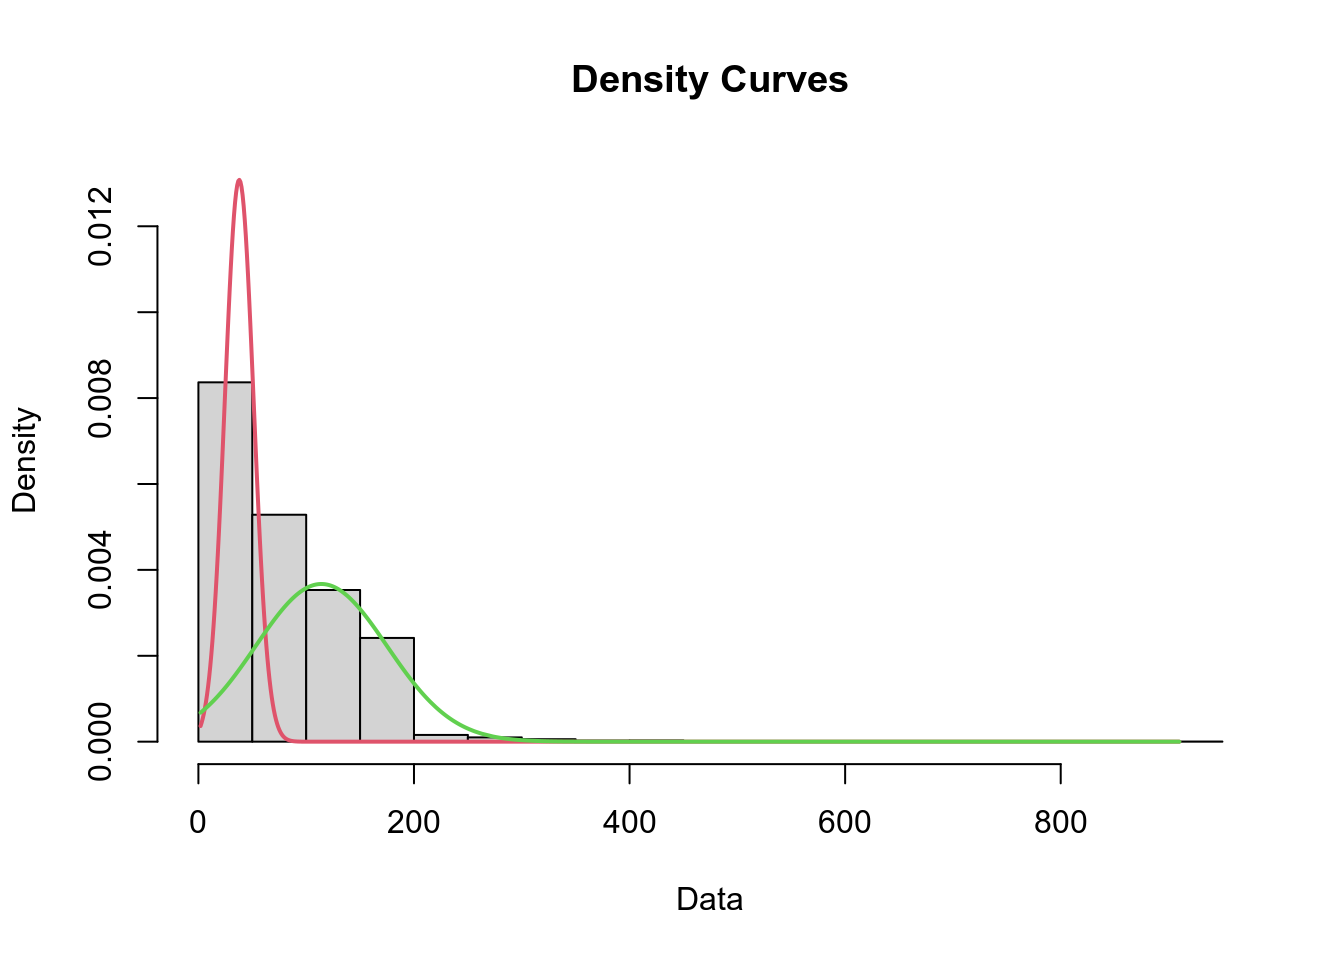
\includegraphics{da4l_files/figure-latex/unnamed-chunk-58-2.pdf}

Однако, если хочется больше контроля над получаемым разультатом, я бы предложил использовать \texttt{ggplot()}:

\begin{Shaded}
\begin{Highlighting}[]
\NormalTok{new\_dnorm }\OtherTok{\textless{}{-}} \ControlFlowTok{function}\NormalTok{(x, mu, sigma, lambda)\{}
  \FunctionTok{dnorm}\NormalTok{(x, mu, sigma)}\SpecialCharTok{*}\NormalTok{lambda}
\NormalTok{\}}

\NormalTok{spam\_sms }\SpecialCharTok{\%\textgreater{}\%} 
  \FunctionTok{ggplot}\NormalTok{(}\FunctionTok{aes}\NormalTok{(n\_char))}\SpecialCharTok{+}
  \FunctionTok{geom\_histogram}\NormalTok{(}\FunctionTok{aes}\NormalTok{(}\AttributeTok{y =}\NormalTok{ ..density..), }\AttributeTok{fill =} \StringTok{"gray90"}\NormalTok{)}\SpecialCharTok{+}
  \FunctionTok{stat\_function}\NormalTok{(}\AttributeTok{fun =}\NormalTok{ new\_dnorm, }
                \AttributeTok{args =} \FunctionTok{c}\NormalTok{(}\AttributeTok{mu =}\NormalTok{ spam\_length\_est}\SpecialCharTok{$}\NormalTok{mu[}\DecValTok{1}\NormalTok{],}
                                          \AttributeTok{sigma =}\NormalTok{ spam\_length\_est}\SpecialCharTok{$}\NormalTok{sigma[}\DecValTok{1}\NormalTok{],}
                                          \AttributeTok{lambda =}\NormalTok{ spam\_length\_est}\SpecialCharTok{$}\NormalTok{lambda[}\DecValTok{1}\NormalTok{]),}
                \AttributeTok{color =} \StringTok{"\#F8766D"}\NormalTok{)}\SpecialCharTok{+}
  \FunctionTok{stat\_function}\NormalTok{(}\AttributeTok{fun =}\NormalTok{ new\_dnorm, }
                \AttributeTok{args =} \FunctionTok{c}\NormalTok{(}\AttributeTok{mu =}\NormalTok{ spam\_length\_est}\SpecialCharTok{$}\NormalTok{mu[}\DecValTok{2}\NormalTok{],}
                                          \AttributeTok{sigma =}\NormalTok{ spam\_length\_est}\SpecialCharTok{$}\NormalTok{sigma[}\DecValTok{2}\NormalTok{],}
                                          \AttributeTok{lambda =}\NormalTok{ spam\_length\_est}\SpecialCharTok{$}\NormalTok{lambda[}\DecValTok{2}\NormalTok{]),}
                \AttributeTok{color =} \StringTok{"\#00BFC4"}\NormalTok{)}\SpecialCharTok{+}
  \FunctionTok{labs}\NormalTok{(}\AttributeTok{caption =} \StringTok{"данные из kaggle.com/uciml/sms{-}spam{-}collection{-}dataset"}\NormalTok{,}
       \AttributeTok{x =} \StringTok{"количество символов"}\NormalTok{,}
       \AttributeTok{y =} \StringTok{"значение функции плотности"}\NormalTok{)}\SpecialCharTok{+}
  \FunctionTok{geom\_vline}\NormalTok{(}\AttributeTok{xintercept =} \DecValTok{160}\NormalTok{, }\AttributeTok{linetype =} \DecValTok{2}\NormalTok{, }\AttributeTok{size =} \FloatTok{0.3}\NormalTok{)}
\end{Highlighting}
\end{Shaded}

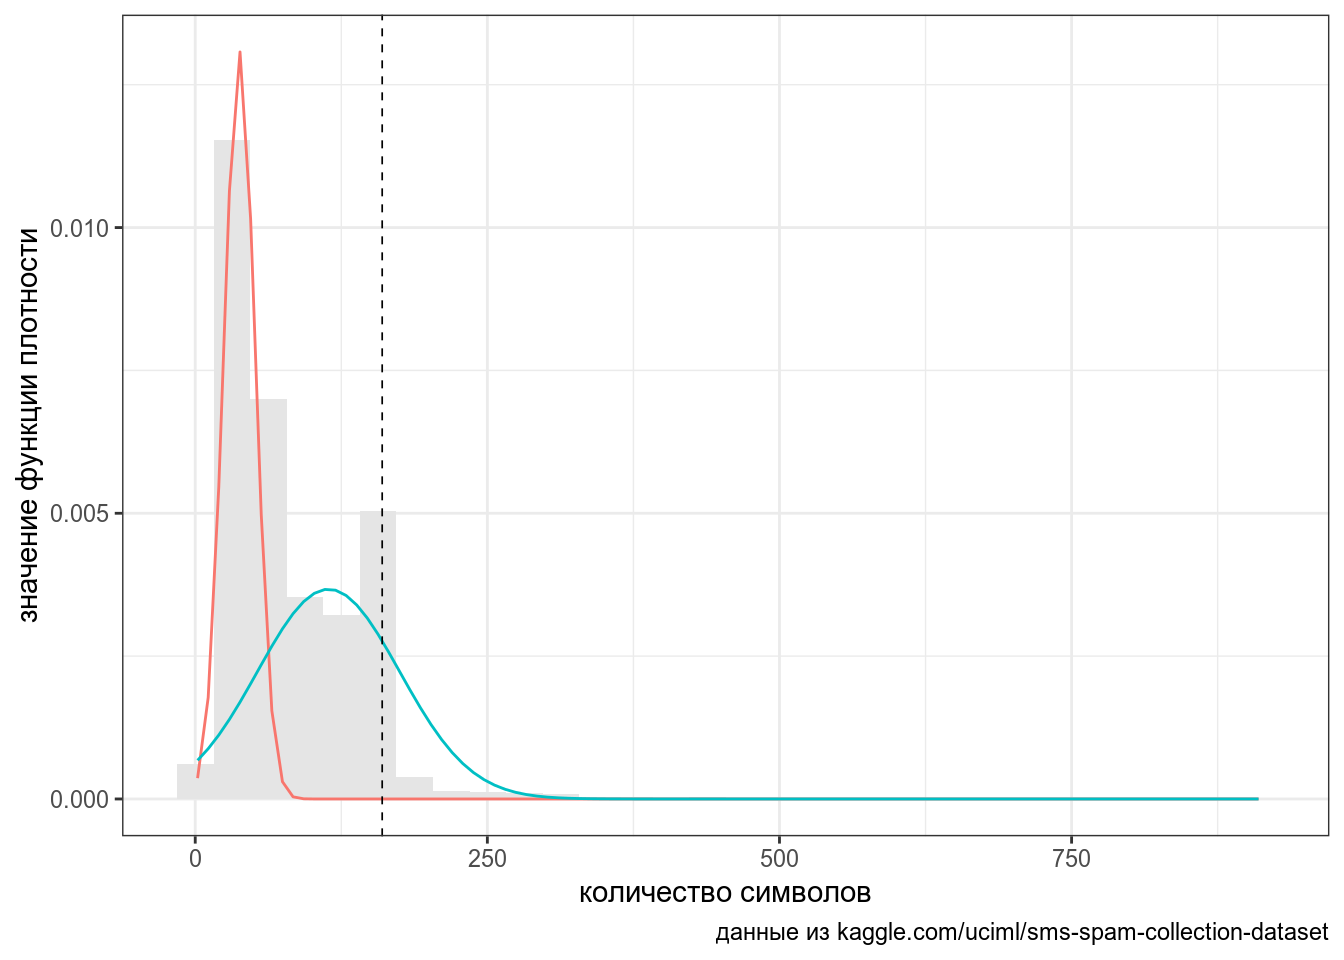
\includegraphics{da4l_files/figure-latex/unnamed-chunk-59-1.pdf}

Таким образом мы получили классификатор

\begin{Shaded}
\begin{Highlighting}[]
\NormalTok{first }\OtherTok{\textless{}{-}} \FunctionTok{new\_dnorm}\NormalTok{(}\FunctionTok{seq}\NormalTok{(}\DecValTok{1}\NormalTok{, }\DecValTok{750}\NormalTok{, }\AttributeTok{by =} \DecValTok{1}\NormalTok{), }
                   \AttributeTok{mu =}\NormalTok{ spam\_length\_est}\SpecialCharTok{$}\NormalTok{mu[}\DecValTok{1}\NormalTok{],}
                   \AttributeTok{sigma =}\NormalTok{ spam\_length\_est}\SpecialCharTok{$}\NormalTok{sigma[}\DecValTok{1}\NormalTok{],}
                   \AttributeTok{lambda =}\NormalTok{ spam\_length\_est}\SpecialCharTok{$}\NormalTok{lambda[}\DecValTok{1}\NormalTok{])}
\NormalTok{second }\OtherTok{\textless{}{-}} \FunctionTok{new\_dnorm}\NormalTok{(}\FunctionTok{seq}\NormalTok{(}\DecValTok{1}\NormalTok{, }\DecValTok{750}\NormalTok{, }\AttributeTok{by =} \DecValTok{1}\NormalTok{), }
                    \AttributeTok{mu =}\NormalTok{ spam\_length\_est}\SpecialCharTok{$}\NormalTok{mu[}\DecValTok{2}\NormalTok{],}
                    \AttributeTok{sigma =}\NormalTok{ spam\_length\_est}\SpecialCharTok{$}\NormalTok{sigma[}\DecValTok{2}\NormalTok{],}
                    \AttributeTok{lambda =}\NormalTok{ spam\_length\_est}\SpecialCharTok{$}\NormalTok{lambda[}\DecValTok{2}\NormalTok{])}
\FunctionTok{which}\NormalTok{(first }\SpecialCharTok{\textgreater{}}\NormalTok{ second)}
\end{Highlighting}
\end{Shaded}

\begin{verbatim}
 [1]  6  7  8  9 10 11 12 13 14 15 16 17 18 19 20 21 22 23 24 25 26 27 28 29 30
[26] 31 32 33 34 35 36 37 38 39 40 41 42 43 44 45 46 47 48 49 50 51 52 53 54 55
[51] 56 57 58 59 60 61 62
\end{verbatim}

Если в смс-сообщении больше 62 символов, то согласно нашей модели, вероятнее всего это спам.

\begin{Shaded}
\begin{Highlighting}[]
\NormalTok{spam\_sms }\SpecialCharTok{\%\textgreater{}\%} 
  \FunctionTok{mutate}\NormalTok{(}\AttributeTok{model\_predict =} \FunctionTok{ifelse}\NormalTok{(n\_char }\SpecialCharTok{\textgreater{}} \DecValTok{63}\NormalTok{, }\StringTok{"predicted\_spam"}\NormalTok{, }\StringTok{"predicted\_ham"}\NormalTok{)) }\SpecialCharTok{\%\textgreater{}\%} 
  \FunctionTok{count}\NormalTok{(model\_predict, type) }\SpecialCharTok{\%\textgreater{}\%} 
  \FunctionTok{pivot\_wider}\NormalTok{(}\AttributeTok{names\_from =}\NormalTok{ type, }\AttributeTok{values\_from =}\NormalTok{ n)}
\end{Highlighting}
\end{Shaded}

\begin{verbatim}
# A tibble: 2 x 3
  model_predict    ham  spam
  <chr>          <int> <int>
1 predicted_ham   2834    25
2 predicted_spam  1991   722
\end{verbatim}

Результат не идеальный, но лучше чем помечать как спам каждое 13 сообщение (\(747/(4825+747)\)).

\begin{rmdtask}
В работе {[}@coretta2016{]} собраны
\href{https://raw.githubusercontent.com/agricolamz/2021_da4l/master/data/Coretta_2017_icelandic.csv}{данные}
длительности исландских гласных. Отфильтруйте данные, оставив наблюдения
гласного {[}a{]} (переменная \texttt{vowel}), произнесенные носителем
\texttt{tt01} (переменная \texttt{speaker}) и постройте следующие
графики, моделируя длительность гласного (переменная \texttt{vowel.dur})
смесью трех нормальных распределений. Как вам кажется, насколько хорошо
модель смеси справилась с заданием?
\end{rmdtask}

\begin{verbatim}
number of iterations= 114 
\end{verbatim}

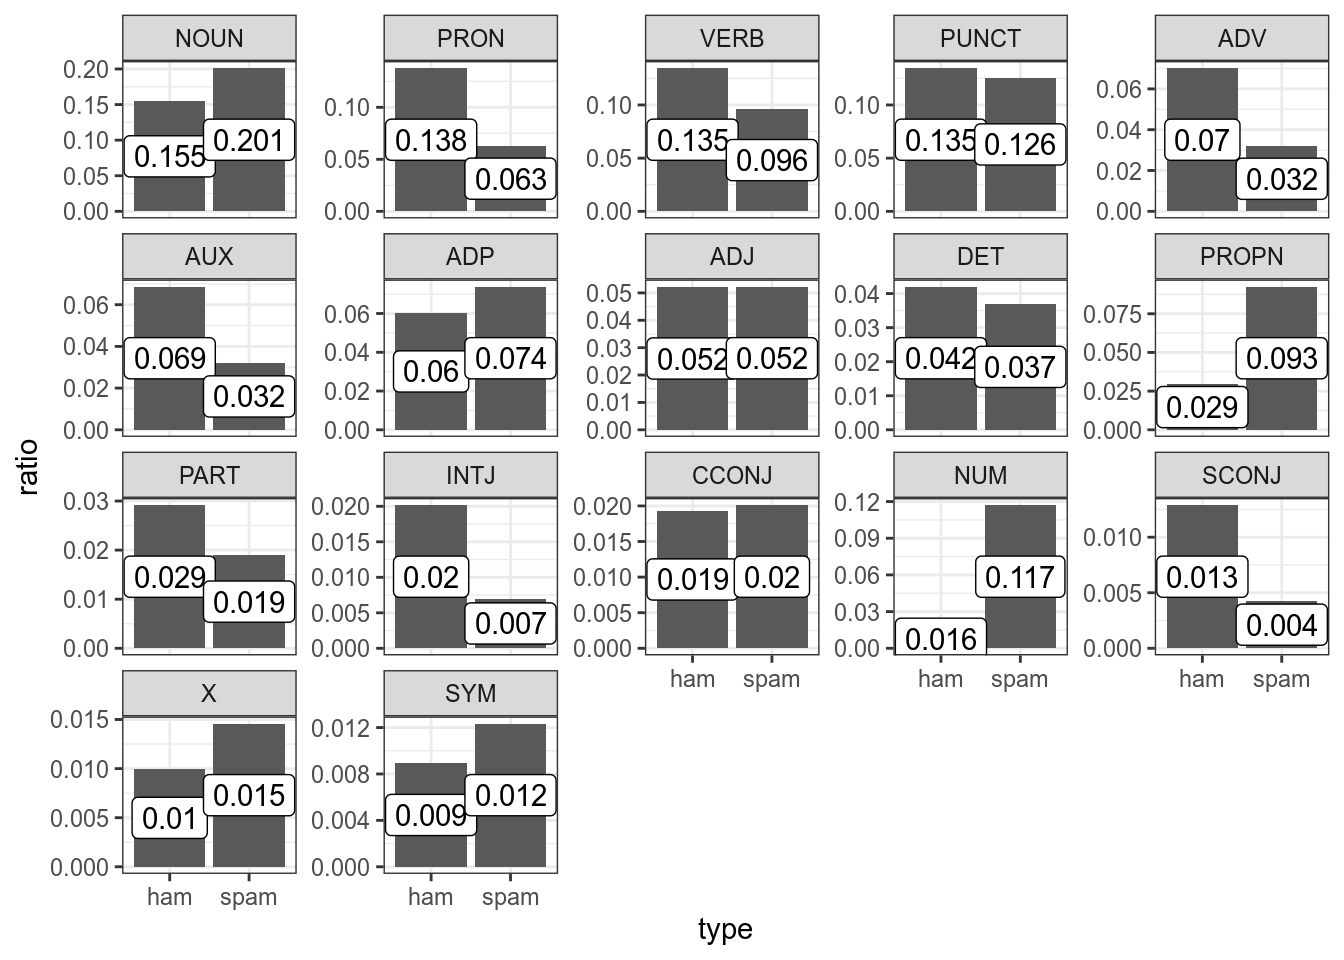
\includegraphics{da4l_files/figure-latex/unnamed-chunk-63-1.pdf} 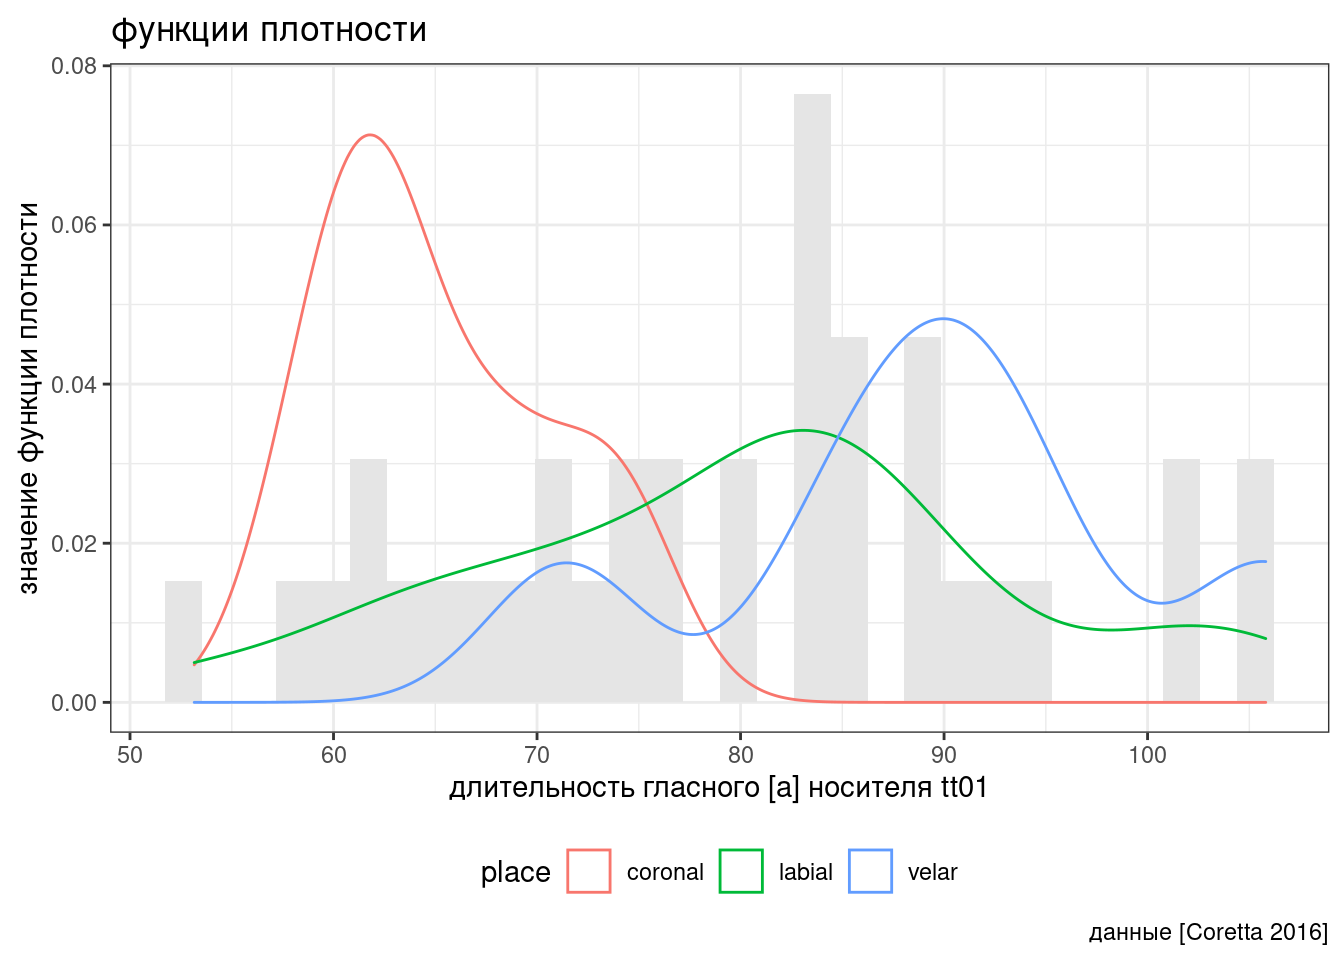
\includegraphics{da4l_files/figure-latex/unnamed-chunk-63-2.pdf}

\hypertarget{ux43dux435ux441ux43aux43eux43bux44cux43aux43e-ux437ux430ux43cux435ux447ux430ux43dux438ux439}{%
\section{Несколько замечаний}\label{ux43dux435ux441ux43aux43eux43bux44cux43aux43e-ux437ux430ux43cux435ux447ux430ux43dux438ux439}}

\begin{itemize}
\tightlist
\item
  В наших примерах нам была доступна информация о классах (spam/ham, coronal/labial/velar), однако модель смесей распределений как раз имеет смысл применять, когда такой информации нет.
\item
  В смеси распределений может быть любое количество распределений.
\item
  Модели смеси распределений не ограничены только нормальным распределением, алгоритм можно использовать и для других распределений.
\item
  Чаще всего в моделях смеси распределений используются распределения одного семейства, однако можно себе представить и комбинации посложнее.
\item
  Модели смеси распределений (mixture models) не стоит путать со смешанными моделями (mixed effects models).
\end{itemize}

\hypertarget{ux431ux430ux439ux435ux441ux43eux432ux441ux43aux438ux439-ux441ux442ux430ux442ux438ux441ux442ux438ux447ux435ux441ux43aux438ux439-ux432ux44bux432ux43eux434}{%
\chapter{Байесовский статистический вывод}\label{ux431ux430ux439ux435ux441ux43eux432ux441ux43aux438ux439-ux441ux442ux430ux442ux438ux441ux442ux438ux447ux435ux441ux43aux438ux439-ux432ux44bux432ux43eux434}}

\hypertarget{ux43dux43eux442ux430ux446ux438ux44f}{%
\section{Нотация}\label{ux43dux43eux442ux430ux446ux438ux44f}}

В байесовском подходе статистический вывод описывается формулой Байеса

\[P(θ|Data) = \frac{P(Data|θ)\times P(θ)}{P(Data)}\]

\begin{itemize}
\tightlist
\item
  \(P(θ|Data)\) --- апостериорная вероятность (posterior)
\item
  \(P(Data|θ)\) --- функция правдоподобия (likelihood)
\item
  \(P(θ)\) --- априорная вероятность (prior)
\item
  \(P(Data)\) --- нормализующий делитель
\end{itemize}

В литературе можно еще встретить такую запись:

\[P(θ|Data) \propto P(Data|θ)\times P(θ)\]

На прошлых занятиях мы говорили, что \href{https://stats.stackexchange.com/a/31241/225843}{функция правдоподобия не обязана интегрироваться до 1}, тогда почему, назвав часть формулы Байеса \(P(Data|θ)\) функцией правдоподобия, мы оставляем нотацию, будто это функция вероятностей? Потому что это условная вероятность, \href{https://stats.stackexchange.com/q/448852/225843}{она не обязана интегрироваться до 1}.

\hypertarget{ux43aux430ux442ux435ux433ux43eux440ux438ux430ux43bux44cux43dux44bux439-ux43fux440ux438ux43cux435ux440}{%
\section{Категориальный пример}\label{ux43aux430ux442ux435ux433ux43eux440ux438ux430ux43bux44cux43dux44bux439-ux43fux440ux438ux43cux435ux440}}

Для примера я взял датасет, который содержит спамерские и обычные смс-сообщения, выложенный UCI Machine Learning \href{https://www.kaggle.com/uciml/sms-spam-collection-dataset}{на kaggle} и при помощи пакета \texttt{udpipe} токенизировал и определил часть речи:

\begin{Shaded}
\begin{Highlighting}[]
\NormalTok{sms\_pos }\OtherTok{\textless{}{-}} \FunctionTok{read\_csv}\NormalTok{(}\StringTok{"https://raw.githubusercontent.com/agricolamz/2021\_da4l/master/data/spam\_sms\_pos.csv"}\NormalTok{)}
\FunctionTok{glimpse}\NormalTok{(sms\_pos)}
\end{Highlighting}
\end{Shaded}

\begin{verbatim}
Rows: 34
Columns: 3
$ type <chr> "ham", "ham", "ham", "ham", "ham", "ham", "ham", "ham", "ham",...
$ upos <chr> "ADJ", "ADP", "ADV", "AUX", "CCONJ", "DET", "INTJ", "NOUN", "N...
$ n    <dbl> 4329, 5004, 5832, 5707, 1607, 3493, 1676, 12842, 1293, 2424, 1...
\end{verbatim}

\begin{Shaded}
\begin{Highlighting}[]
\NormalTok{sms\_pos }\SpecialCharTok{\%\textgreater{}\%} 
  \FunctionTok{group\_by}\NormalTok{(type) }\SpecialCharTok{\%\textgreater{}\%} 
  \FunctionTok{mutate}\NormalTok{(}\AttributeTok{ratio =}\NormalTok{ n}\SpecialCharTok{/}\FunctionTok{sum}\NormalTok{(n),}
         \AttributeTok{upos =} \FunctionTok{fct\_reorder}\NormalTok{(upos, n, mean, }\AttributeTok{.desc =} \ConstantTok{TRUE}\NormalTok{)) }\SpecialCharTok{\%\textgreater{}\%}
  \FunctionTok{ggplot}\NormalTok{(}\FunctionTok{aes}\NormalTok{(type, ratio))}\SpecialCharTok{+}
  \FunctionTok{geom\_col}\NormalTok{()}\SpecialCharTok{+}
  \FunctionTok{geom\_label}\NormalTok{(}\FunctionTok{aes}\NormalTok{(}\AttributeTok{label =} \FunctionTok{round}\NormalTok{(ratio, }\DecValTok{3}\NormalTok{)), }\AttributeTok{position =} \FunctionTok{position\_stack}\NormalTok{(}\AttributeTok{vjust =} \FloatTok{0.5}\NormalTok{))}\SpecialCharTok{+}
  \FunctionTok{facet\_wrap}\NormalTok{(}\SpecialCharTok{\textasciitilde{}}\NormalTok{upos, }\AttributeTok{scales =} \StringTok{"free\_y"}\NormalTok{)}
\end{Highlighting}
\end{Shaded}

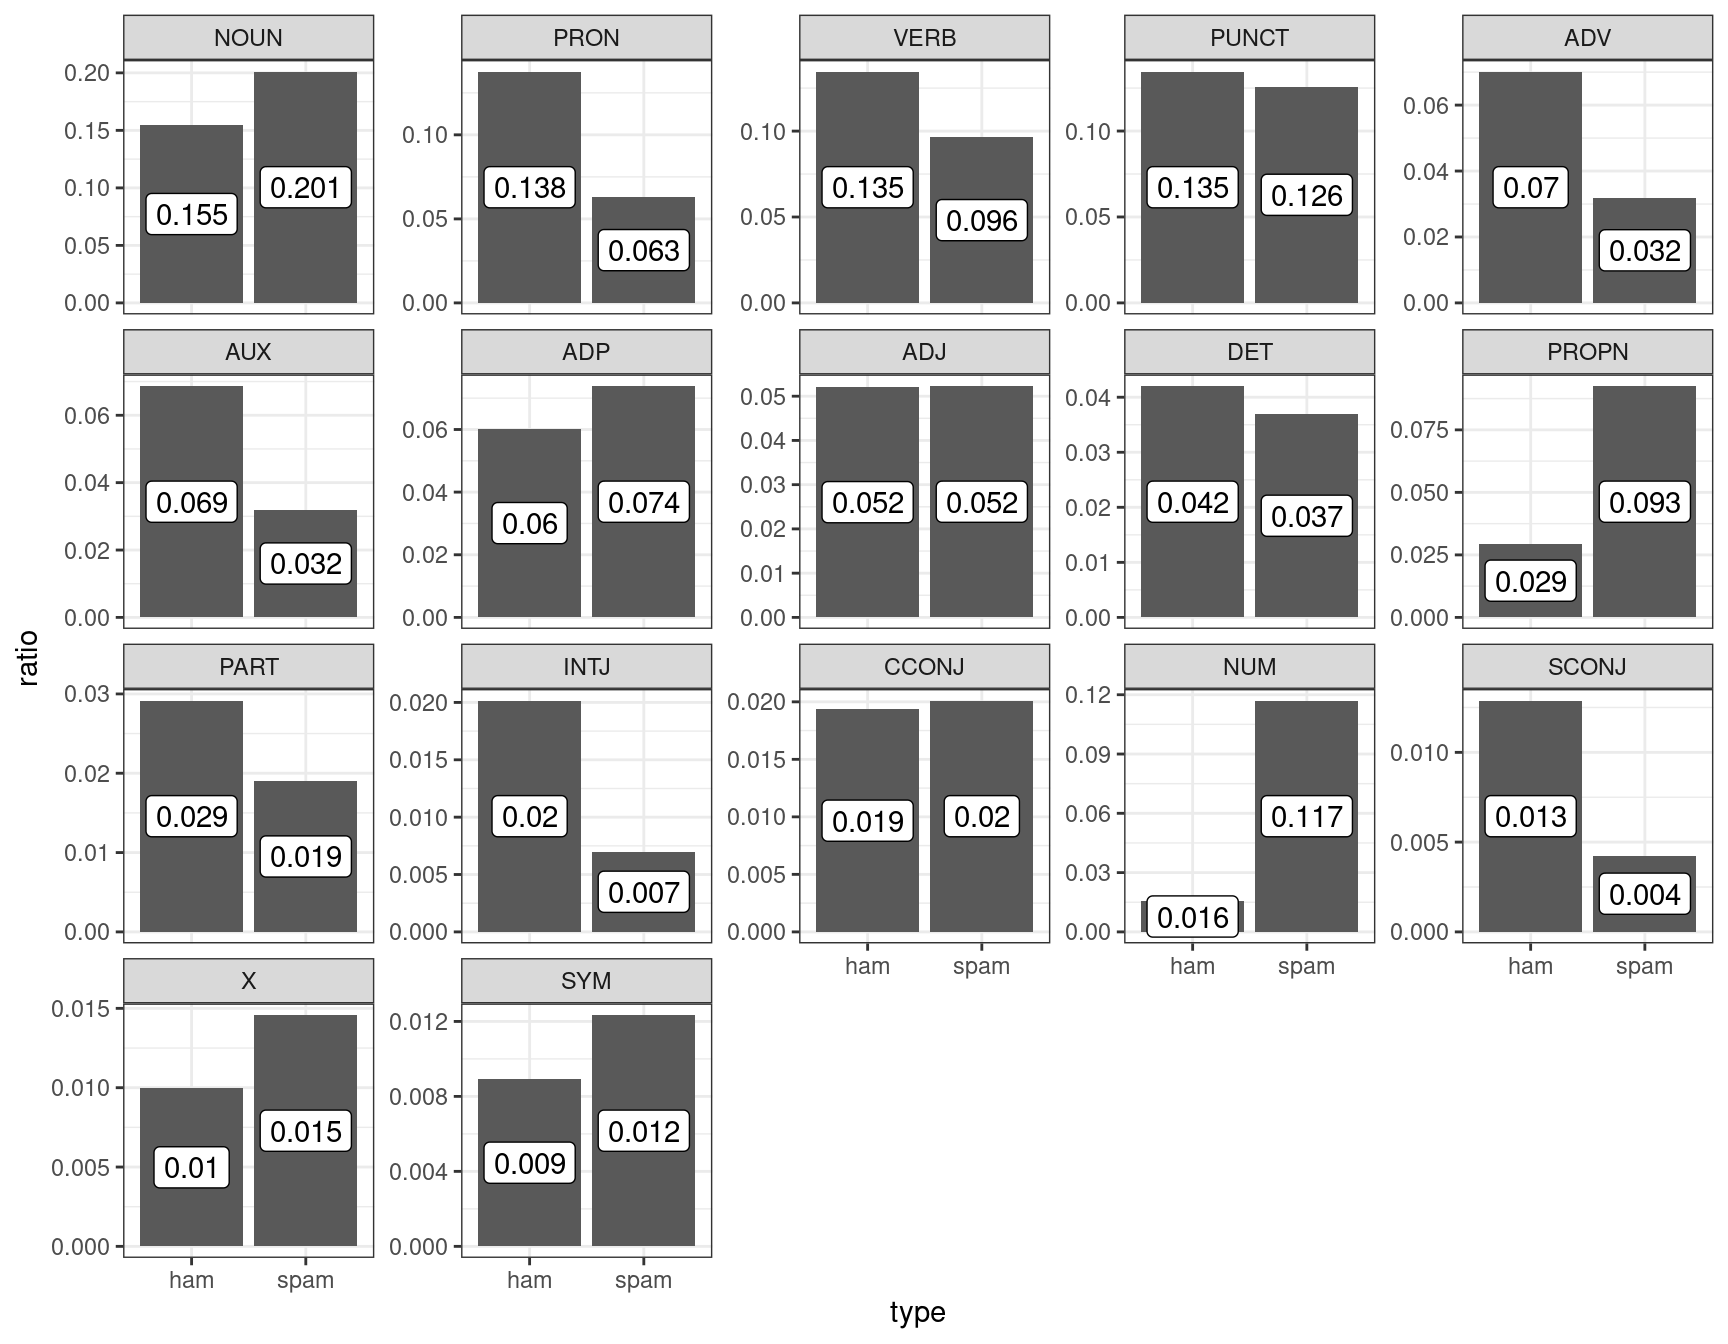
\includegraphics{da4l_files/figure-latex/unnamed-chunk-64-1.pdf}

Давайте полученные доли считать нашей моделью: сумма всех чисел внутри каждого типа (\texttt{ham}/\texttt{spam}) дает в сумме 1. Мы получили новое сообщение:

\begin{quote}
Call FREEPHONE 0800 542 0825 now!
\end{quote}

Модель \texttt{udpipe} разобрала его следующим образом:

\begin{quote}
VERB NUM NUM NUM NUM ADV PUNCT
\end{quote}

Понятно, что это -- спам, но мы попытаемся применить байесовский статистический вывод, чтобы определить тип сообщения. Предположим, что машина считает обе гипотезы равновероятными, т. е. ее априорное распределение гипотез равно 0.5 каждая. На минуту представим, что машина анализирует текст пословно. Первое слово типа \texttt{VERB}. Функции правдоподобия равны 0.135 и 0.096 для сообщений типа \texttt{ham} и \texttt{spam} соответственно. Применим байесовский апдейт:

\begin{Shaded}
\begin{Highlighting}[]
\FunctionTok{tibble}\NormalTok{(}\AttributeTok{model =} \FunctionTok{c}\NormalTok{(}\StringTok{"ham"}\NormalTok{, }\StringTok{"spam"}\NormalTok{),}
       \AttributeTok{prior =} \FloatTok{0.5}\NormalTok{,}
       \AttributeTok{likelihood =} \FunctionTok{c}\NormalTok{(}\FloatTok{0.135}\NormalTok{, }\FloatTok{0.096}\NormalTok{),}
       \AttributeTok{product =}\NormalTok{ prior}\SpecialCharTok{*}\NormalTok{likelihood,}
       \AttributeTok{posterior =}\NormalTok{ product}\SpecialCharTok{/}\FunctionTok{sum}\NormalTok{(product))}
\end{Highlighting}
\end{Shaded}

\begin{verbatim}
# A tibble: 2 x 5
  model prior likelihood product posterior
  <chr> <dbl>      <dbl>   <dbl>     <dbl>
1 ham     0.5      0.135  0.0675     0.584
2 spam    0.5      0.096  0.048      0.416
\end{verbatim}

Вот мы и сделали байесовский апдейт. Теперь апостериорное распределение, которое мы получили на предыдущем шаге, мы можем использовать в новом апдейте. Следующее слово в сообщении типа \texttt{NUM}.

\begin{Shaded}
\begin{Highlighting}[]
\FunctionTok{tibble}\NormalTok{(}\AttributeTok{model =} \FunctionTok{c}\NormalTok{(}\StringTok{"ham"}\NormalTok{, }\StringTok{"spam"}\NormalTok{),}
       \AttributeTok{prior\_2 =} \FunctionTok{c}\NormalTok{(}\FloatTok{0.584}\NormalTok{, }\FloatTok{0.416}\NormalTok{),}
       \AttributeTok{likelihood\_2 =} \FunctionTok{c}\NormalTok{(}\FloatTok{0.016}\NormalTok{, }\FloatTok{0.117}\NormalTok{),}
       \AttributeTok{product\_2 =}\NormalTok{ prior\_2}\SpecialCharTok{*}\NormalTok{likelihood\_2,}
       \AttributeTok{posterior\_2 =}\NormalTok{ product\_2}\SpecialCharTok{/}\FunctionTok{sum}\NormalTok{(product\_2))}
\end{Highlighting}
\end{Shaded}

\begin{verbatim}
# A tibble: 2 x 5
  model prior_2 likelihood_2 product_2 posterior_2
  <chr>   <dbl>        <dbl>     <dbl>       <dbl>
1 ham     0.584        0.016   0.00934       0.161
2 spam    0.416        0.117   0.0487        0.839
\end{verbatim}

Уже на второй итерации, наша модель почти уверена, что это сообщение \texttt{spam}. На третьей итерации уверенность только растет:

\begin{Shaded}
\begin{Highlighting}[]
\FunctionTok{tibble}\NormalTok{(}\AttributeTok{model =} \FunctionTok{c}\NormalTok{(}\StringTok{"ham"}\NormalTok{, }\StringTok{"spam"}\NormalTok{),}
       \AttributeTok{prior\_3 =} \FunctionTok{c}\NormalTok{(}\FloatTok{0.161}\NormalTok{, }\FloatTok{0.839}\NormalTok{),}
       \AttributeTok{likelihood\_3 =} \FunctionTok{c}\NormalTok{(}\FloatTok{0.016}\NormalTok{, }\FloatTok{0.117}\NormalTok{),}
       \AttributeTok{product\_3 =}\NormalTok{ prior\_3}\SpecialCharTok{*}\NormalTok{likelihood\_3,}
       \AttributeTok{posterior\_3 =}\NormalTok{ product\_3}\SpecialCharTok{/}\FunctionTok{sum}\NormalTok{(product\_3))}
\end{Highlighting}
\end{Shaded}

\begin{verbatim}
# A tibble: 2 x 5
  model prior_3 likelihood_3 product_3 posterior_3
  <chr>   <dbl>        <dbl>     <dbl>       <dbl>
1 ham     0.161        0.016   0.00258      0.0256
2 spam    0.839        0.117   0.0982       0.974 
\end{verbatim}

\begin{rmdtask}
Посчитайте вероятность гипотезы, что перед нами спамерское сообщение,
если предположить, что каждое пятое сообщение -- спам. Ответ округлите
до трех знаков после запятой.
\end{rmdtask}

Из формулы Байеса следует, что не обязательно каждый раз делить на нормализующий делитель, это можно сделать единожды.

\begin{Shaded}
\begin{Highlighting}[]
\FunctionTok{tibble}\NormalTok{(}\AttributeTok{model =} \FunctionTok{c}\NormalTok{(}\StringTok{"ham"}\NormalTok{, }\StringTok{"spam"}\NormalTok{),}
       \AttributeTok{prior =} \FloatTok{0.5}\NormalTok{,}
       \AttributeTok{likelihood =} \FunctionTok{c}\NormalTok{(}\FloatTok{0.135}\NormalTok{, }\FloatTok{0.096}\NormalTok{),}
       \AttributeTok{likelihood\_2 =} \FunctionTok{c}\NormalTok{(}\FloatTok{0.016}\NormalTok{, }\FloatTok{0.117}\NormalTok{),}
       \AttributeTok{product =}\NormalTok{ prior}\SpecialCharTok{*}\NormalTok{likelihood}\SpecialCharTok{*}\NormalTok{likelihood\_2}\SpecialCharTok{*}\NormalTok{likelihood\_2,}
       \AttributeTok{posterior =}\NormalTok{ product}\SpecialCharTok{/}\FunctionTok{sum}\NormalTok{(product))}
\end{Highlighting}
\end{Shaded}

\begin{verbatim}
# A tibble: 2 x 6
  model prior likelihood likelihood_2   product posterior
  <chr> <dbl>      <dbl>        <dbl>     <dbl>     <dbl>
1 ham     0.5      0.135        0.016 0.0000173    0.0256
2 spam    0.5      0.096        0.117 0.000657     0.974 
\end{verbatim}

Из приведенных рассуждений также следует, что все равно в каком порядке мы производим байесовский апдейт: мы могли сначала умножить на значение правдоподобия для категории \texttt{NUM} и лишь в конце на значение правдоподобия \texttt{VERB}.

Также стоит отметить, что если данных много, то через какое-то время становится все равно, какое у нас было априорное распределение. Даже в нашем примере, в котором мы проанализировали первые три слова сообщения, модель, прогнозирующая, что сообщение спамерское, выиграет, даже если, согласно априорному распределению, спамерским является каждое 20 сообщение:

\begin{Shaded}
\begin{Highlighting}[]
\FunctionTok{tibble}\NormalTok{(}\AttributeTok{model =} \FunctionTok{c}\NormalTok{(}\StringTok{"ham"}\NormalTok{, }\StringTok{"spam"}\NormalTok{),}
       \AttributeTok{prior =} \FunctionTok{c}\NormalTok{(}\FloatTok{0.95}\NormalTok{, }\FloatTok{0.05}\NormalTok{),}
       \AttributeTok{likelihood =} \FunctionTok{c}\NormalTok{(}\FloatTok{0.135}\NormalTok{, }\FloatTok{0.096}\NormalTok{),}
       \AttributeTok{likelihood\_2 =} \FunctionTok{c}\NormalTok{(}\FloatTok{0.016}\NormalTok{, }\FloatTok{0.117}\NormalTok{),}
       \AttributeTok{product =}\NormalTok{ prior}\SpecialCharTok{*}\NormalTok{likelihood}\SpecialCharTok{*}\NormalTok{likelihood\_2}\SpecialCharTok{*}\NormalTok{likelihood\_2,}
       \AttributeTok{posterior =}\NormalTok{ product}\SpecialCharTok{/}\FunctionTok{sum}\NormalTok{(product))}
\end{Highlighting}
\end{Shaded}

\begin{verbatim}
# A tibble: 2 x 6
  model prior likelihood likelihood_2   product posterior
  <chr> <dbl>      <dbl>        <dbl>     <dbl>     <dbl>
1 ham    0.95      0.135        0.016 0.0000328     0.333
2 spam   0.05      0.096        0.117 0.0000657     0.667
\end{verbatim}

Самым главным отличием байесовского статистического вывода от фриквентистского, является то, что мы в результате получаем вероятность каждой из моделей. Это очень значительно отличается от фриквентистской практики нулевых гипотез и p-value, в соответствии с которыми мы можем лишь отвергнуть или не отвергнуть нулевую гипотезу.

\begin{rmdtask}
Вашего друга похитили а на почту отправили
\href{https://raw.githubusercontent.com/agricolamz/2021_da4l/master/data/weather.csv}{датасет},
в котором записаны данные о погоде из пяти городов. Ваш телефон
зазвонил, и друг сказал, что не знает куда его похитили, но за окном
легкий дождь (\texttt{Rain}). А в какой-то из следующих дней --- сильный
дождь (\texttt{Rain,\ Thunderstorm}). Исходя из явно неверного
предположения, что погодные условия каждый день не зависят друг от
друга, сделайте байесовский апдейт и предположите, в какой город
вероятнее всего похитили друга.
\end{rmdtask}

\begin{rmdtask}
Укажите получившуюся вероятность. Выполняя задание, округлите все
вероятности и значения правдоподобия до 3 знаков после запятой.
\end{rmdtask}

\hypertarget{ux440ux430ux437ux43dux438ux446ux430-ux43cux435ux436ux434ux443-ux444ux440ux438ux43aux432ux435ux43dux442ux438ux441ux43aux438ux43c-ux438-ux431ux430ux439ux435ux441ux43eux432ux441ux43aux438ux43c-ux43fux43eux434ux445ux43eux434ux430ux43cux438}{%
\section{Разница между фриквентиским и байесовским подходами}\label{ux440ux430ux437ux43dux438ux446ux430-ux43cux435ux436ux434ux443-ux444ux440ux438ux43aux432ux435ux43dux442ux438ux441ux43aux438ux43c-ux438-ux431ux430ux439ux435ux441ux43eux432ux441ux43aux438ux43c-ux43fux43eux434ux445ux43eux434ux430ux43cux438}}

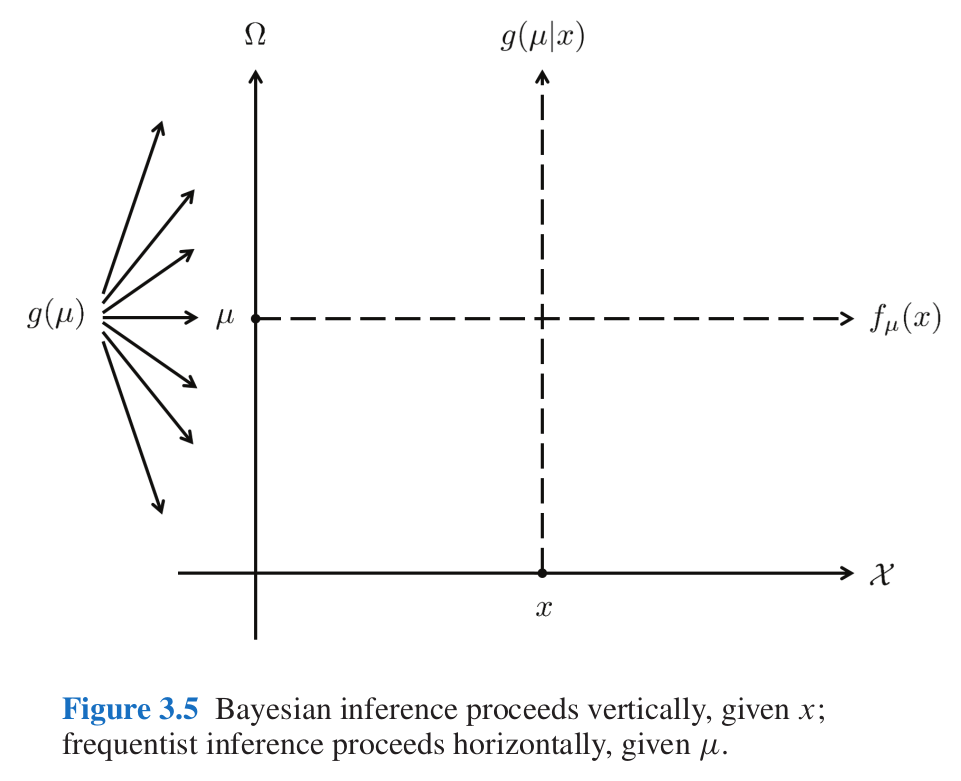
\includegraphics{images/gelman.png}

Картинка из одной из моих любимых книг по статистике \citep[34]{efron16}.

\hypertarget{ux431ux438ux43dux43eux43cux438ux430ux43bux44cux43dux44bux435-ux434ux430ux43dux43dux44bux435}{%
\section{Биномиальные данные}\label{ux431ux438ux43dux43eux43cux438ux430ux43bux44cux43dux44bux435-ux434ux430ux43dux43dux44bux435}}

Биномиальные данные возникают, когда нас интересует доля успехов в какой-то серии эксперементов Бернулли.

\hypertarget{ux431ux438ux43dux43eux43cux438ux430ux43bux44cux43dux43eux435-ux440ux430ux441ux43fux440ux435ux434ux435ux43bux435ux43dux438ux435-1}{%
\subsection{Биномиальное распределение}\label{ux431ux438ux43dux43eux43cux438ux430ux43bux44cux43dux43eux435-ux440ux430ux441ux43fux440ux435ux434ux435ux43bux435ux43dux438ux435-1}}

Биномиальное распределение --- распределение количества успехов эксперементов Бернулли из \emph{n} попыток с вероятностью успеха \emph{p}.

\[P(k | n, p) = \frac{n!}{k!(n-k)!} \times p^k \times (1-p)^{n-k} =  {n \choose k} \times p^k \times (1-p)^{n-k}\]
\[ 0 \leq p \leq 1; n, k > 0\]

\begin{Shaded}
\begin{Highlighting}[]
\FunctionTok{tibble}\NormalTok{(}\AttributeTok{x =} \DecValTok{0}\SpecialCharTok{:}\DecValTok{50}\NormalTok{,}
           \AttributeTok{density =} \FunctionTok{dbinom}\NormalTok{(}\AttributeTok{x =}\NormalTok{ x, }\AttributeTok{size =} \DecValTok{50}\NormalTok{, }\AttributeTok{prob =} \FloatTok{0.16}\NormalTok{)) }\SpecialCharTok{\%\textgreater{}\%} 
  \FunctionTok{ggplot}\NormalTok{(}\FunctionTok{aes}\NormalTok{(x, density))}\SpecialCharTok{+}
  \FunctionTok{geom\_point}\NormalTok{()}\SpecialCharTok{+}
  \FunctionTok{geom\_line}\NormalTok{()}\SpecialCharTok{+}
  \FunctionTok{labs}\NormalTok{(}\AttributeTok{title =} \StringTok{"Биномиальное распределение p = 0.16, n = 50"}\NormalTok{)}
\end{Highlighting}
\end{Shaded}

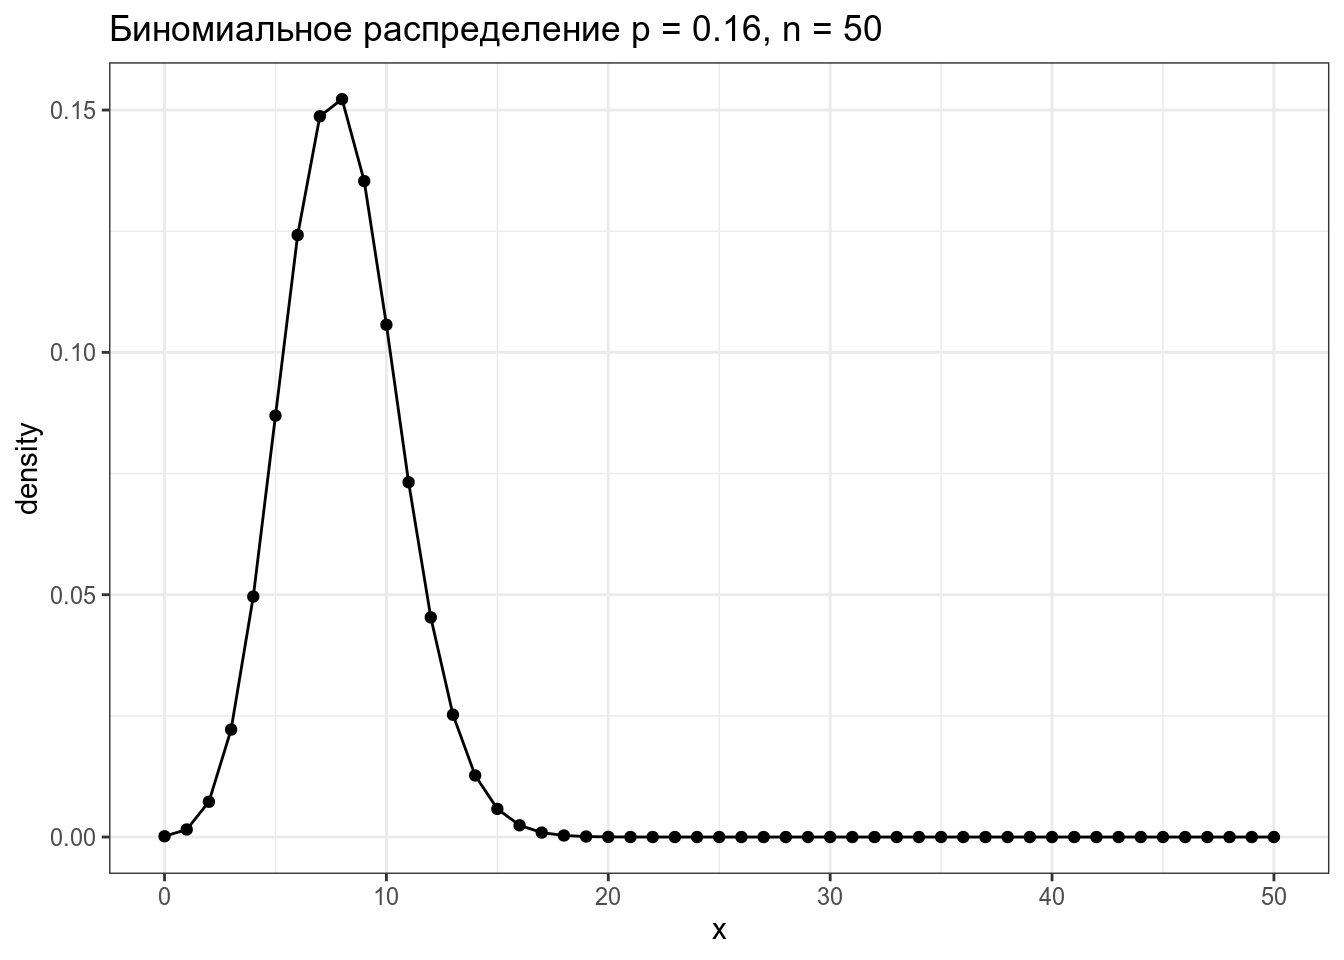
\includegraphics{da4l_files/figure-latex/unnamed-chunk-77-1.pdf}

\hypertarget{ux431ux435ux442ux430-ux440ux430ux441ux43fux440ux435ux434ux435ux43bux435ux43dux438ux435}{%
\subsection{Бета распределение}\label{ux431ux435ux442ux430-ux440ux430ux441ux43fux440ux435ux434ux435ux43bux435ux43dux438ux435}}

\[P(x; α, β) = \frac{x^{α-1}\times (1-x)^{β-1}}{B(α, β)}; 0 \leq x \leq 1; α, β > 0\]

Бета функция:

\[Β(α, β) = \frac{Γ(α)\times Γ(β)}{Γ(α+β)} = \frac{(α-1)!(β-1)!}{(α+β-1)!} \]

\begin{Shaded}
\begin{Highlighting}[]
\FunctionTok{tibble}\NormalTok{(}\AttributeTok{x =} \FunctionTok{seq}\NormalTok{(}\DecValTok{0}\NormalTok{, }\DecValTok{1}\NormalTok{, }\AttributeTok{length.out =} \DecValTok{100}\NormalTok{),}
           \AttributeTok{density =} \FunctionTok{dbeta}\NormalTok{(}\AttributeTok{x =}\NormalTok{ x, }\AttributeTok{shape1 =} \DecValTok{8}\NormalTok{, }\AttributeTok{shape2 =} \DecValTok{42}\NormalTok{)) }\SpecialCharTok{\%\textgreater{}\%} 
  \FunctionTok{ggplot}\NormalTok{(}\FunctionTok{aes}\NormalTok{(x, density))}\SpecialCharTok{+}
  \FunctionTok{geom\_point}\NormalTok{()}\SpecialCharTok{+}
  \FunctionTok{geom\_line}\NormalTok{()}\SpecialCharTok{+}
  \FunctionTok{labs}\NormalTok{(}\AttributeTok{title =} \StringTok{"Бета распределение α = 8, β = 42"}\NormalTok{)}
\end{Highlighting}
\end{Shaded}

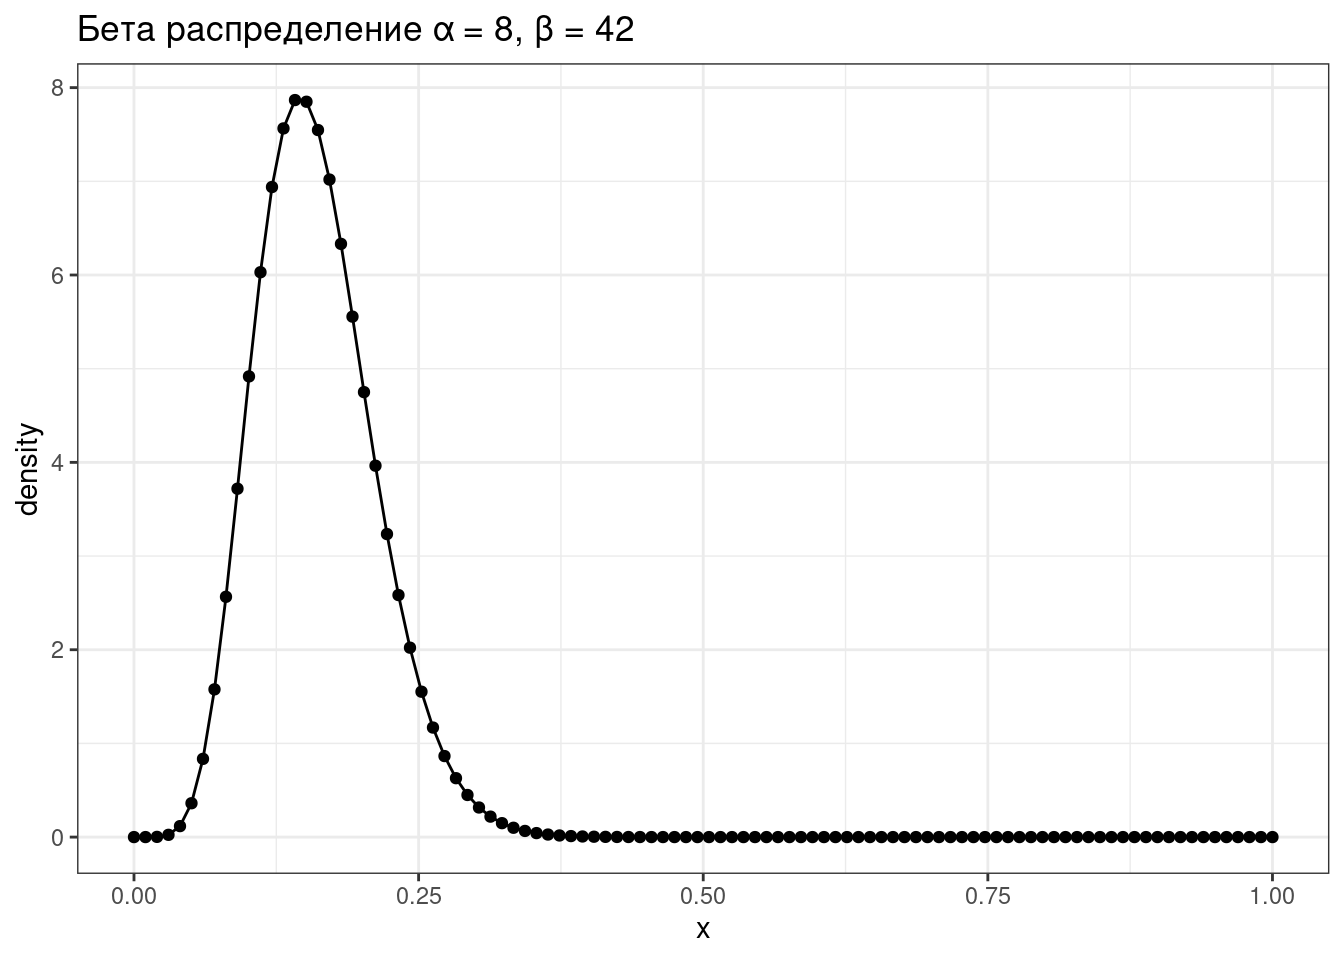
\includegraphics{da4l_files/figure-latex/unnamed-chunk-78-1.pdf}

Можно поиграть с разными параметрами:

\begin{Shaded}
\begin{Highlighting}[]
\NormalTok{shiny}\SpecialCharTok{::}\FunctionTok{runGitHub}\NormalTok{(}\StringTok{"agricolamz/beta\_distribution\_shiny"}\NormalTok{) }
\end{Highlighting}
\end{Shaded}

\[\mu = \frac{\alpha}{\alpha+\beta}\]

\[\sigma^2 = \frac{\alpha\times\beta}{(\alpha+\beta)^2\times(\alpha+\beta+1)}\]

\hypertarget{ux431ux430ux439ux435ux441ux43eux432ux441ux43aux438ux439-ux430ux43fux434ux435ux439ux442-ux431ux438ux43dux43eux43cux438ux430ux43bux44cux43dux44bux445-ux434ux430ux43dux43dux44bux445}{%
\subsection{Байесовский апдейт биномиальных данных}\label{ux431ux430ux439ux435ux441ux43eux432ux441ux43aux438ux439-ux430ux43fux434ux435ux439ux442-ux431ux438ux43dux43eux43cux438ux430ux43bux44cux43dux44bux445-ux434ux430ux43dux43dux44bux445}}

\[Beta_{post}(\alpha_{post}, \beta_{post}) = Beta(\alpha_{prior}+\alpha_{data}, \beta_{prior}+\beta_{data}),\]
где \(Beta\) --- это бета распределение

\begin{Shaded}
\begin{Highlighting}[]
\NormalTok{shiny}\SpecialCharTok{::}\FunctionTok{runGitHub}\NormalTok{(}\StringTok{"agricolamz/bayes\_for\_binomial\_app"}\NormalTok{) }
\end{Highlighting}
\end{Shaded}

\begin{rmdtask}
Немного упрощая данные из статьи {[}@rosenbach03: 394{]}, можно сказать
что носители британского английского предпочитают \emph{s}-генитив
(90\%) \emph{of}-генитиву (10\%). Проведите байесовский апдейт, если Вы
наблюдаете в интервью британского актера из 120 контекстов 92
\emph{s}-генитивов. Априорное распределение берите соразмерное данным.
Ответ округлите до трёх или менее знаков после запятой.
\end{rmdtask}

\begin{rmdtask}
Параметр альфа:
\end{rmdtask}

\begin{rmdtask}
Параметр бета:
\end{rmdtask}

\hypertarget{ux431ux430ux439ux435ux441ux43eux432ux441ux43aux438ux439-ux430ux43fux434ux435ux439ux442-ux431ux438ux43dux43eux43cux438ux430ux43bux44cux43dux44bux445-ux434ux430ux43dux43dux44bux445-ux43dux435ux441ux43aux43eux43bux44cux43aux43e-ux43cux43eux434ux435ux43bux435ux439}{%
\subsection{Байесовский апдейт биномиальных данных: несколько моделей}\label{ux431ux430ux439ux435ux441ux43eux432ux441ux43aux438ux439-ux430ux43fux434ux435ux439ux442-ux431ux438ux43dux43eux43cux438ux430ux43bux44cux43dux44bux445-ux434ux430ux43dux43dux44bux445-ux43dux435ux441ux43aux43eux43bux44cux43aux43e-ux43cux43eux434ux435ux43bux435ux439}}

\begin{Shaded}
\begin{Highlighting}[]
\FunctionTok{tibble}\NormalTok{(}\AttributeTok{x =} \FunctionTok{rep}\NormalTok{(}\FunctionTok{seq}\NormalTok{(}\DecValTok{0}\NormalTok{, }\DecValTok{1}\NormalTok{, }\AttributeTok{length.out =} \DecValTok{100}\NormalTok{), }\DecValTok{6}\NormalTok{),}
           \AttributeTok{density =} \FunctionTok{c}\NormalTok{(}\FunctionTok{dbeta}\NormalTok{(}\FunctionTok{unique}\NormalTok{(x), }\AttributeTok{shape1 =} \DecValTok{8}\NormalTok{, }\AttributeTok{shape2 =} \DecValTok{42}\NormalTok{),}
                       \FunctionTok{dbeta}\NormalTok{(}\FunctionTok{unique}\NormalTok{(x), }\AttributeTok{shape1 =} \DecValTok{16}\NormalTok{, }\AttributeTok{shape2 =} \DecValTok{34}\NormalTok{),}
                       \FunctionTok{dbeta}\NormalTok{(}\FunctionTok{unique}\NormalTok{(x), }\AttributeTok{shape1 =} \DecValTok{24}\NormalTok{, }\AttributeTok{shape2 =} \DecValTok{26}\NormalTok{),}
                       \FunctionTok{dbeta}\NormalTok{(}\FunctionTok{unique}\NormalTok{(x), }\AttributeTok{shape1 =} \DecValTok{8}\SpecialCharTok{+}\DecValTok{4}\NormalTok{, }\AttributeTok{shape2 =} \DecValTok{42}\SpecialCharTok{+}\DecValTok{16}\NormalTok{),}
                       \FunctionTok{dbeta}\NormalTok{(}\FunctionTok{unique}\NormalTok{(x), }\AttributeTok{shape1 =} \DecValTok{16}\SpecialCharTok{+}\DecValTok{4}\NormalTok{, }\AttributeTok{shape2 =} \DecValTok{34}\SpecialCharTok{+}\DecValTok{16}\NormalTok{),}
                       \FunctionTok{dbeta}\NormalTok{(}\FunctionTok{unique}\NormalTok{(x), }\AttributeTok{shape1 =} \DecValTok{24}\SpecialCharTok{+}\DecValTok{4}\NormalTok{, }\AttributeTok{shape2 =} \DecValTok{26}\SpecialCharTok{+}\DecValTok{16}\NormalTok{)),}
           \AttributeTok{type =} \FunctionTok{rep}\NormalTok{(}\FunctionTok{c}\NormalTok{(}\StringTok{"prior"}\NormalTok{, }\StringTok{"prior"}\NormalTok{, }\StringTok{"prior"}\NormalTok{, }\StringTok{"posterior"}\NormalTok{, }\StringTok{"posterior"}\NormalTok{, }\StringTok{"posterior"}\NormalTok{), }\AttributeTok{each =} \DecValTok{100}\NormalTok{),}
           \AttributeTok{dataset =} \FunctionTok{rep}\NormalTok{(}\FunctionTok{c}\NormalTok{(}\StringTok{"prior: 8, 42"}\NormalTok{, }\StringTok{"prior: 16, 34"}\NormalTok{, }\StringTok{"prior: 24, 26"}\NormalTok{,}
                           \StringTok{"prior: 8, 42"}\NormalTok{, }\StringTok{"prior: 16, 34"}\NormalTok{, }\StringTok{"prior: 24, 26"}\NormalTok{), }\AttributeTok{each =} \DecValTok{100}\NormalTok{)) }\SpecialCharTok{\%\textgreater{}\%} 
  \FunctionTok{ggplot}\NormalTok{(}\FunctionTok{aes}\NormalTok{(x, density, }\AttributeTok{color =}\NormalTok{ type))}\SpecialCharTok{+}
  \FunctionTok{geom\_line}\NormalTok{()}\SpecialCharTok{+}
  \FunctionTok{facet\_wrap}\NormalTok{(}\SpecialCharTok{\textasciitilde{}}\NormalTok{dataset)}\SpecialCharTok{+}
  \FunctionTok{labs}\NormalTok{(}\AttributeTok{title =} \StringTok{"data = 4, 16"}\NormalTok{)}
\end{Highlighting}
\end{Shaded}

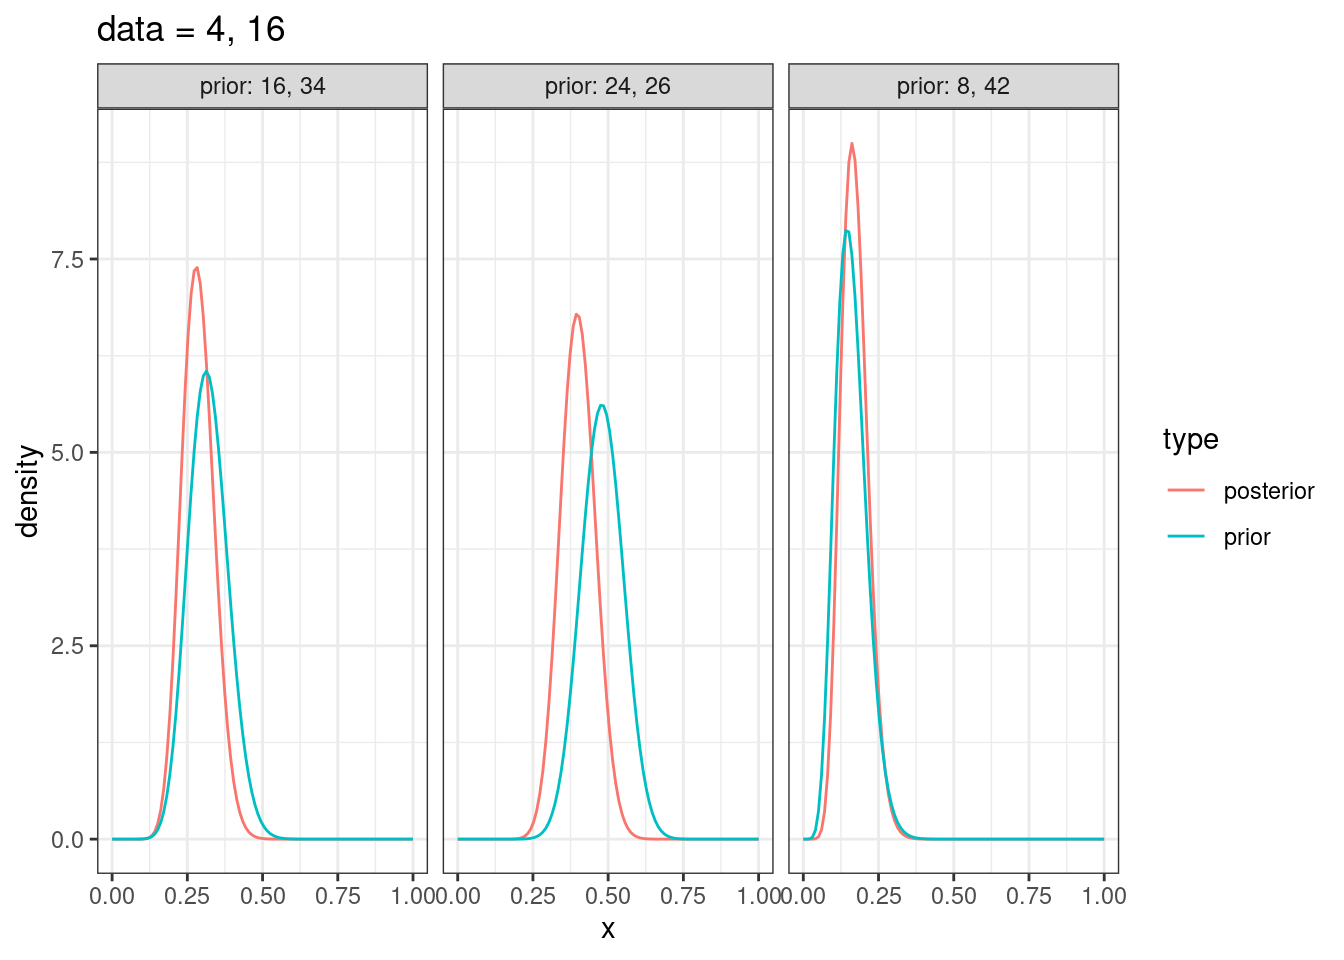
\includegraphics{da4l_files/figure-latex/unnamed-chunk-86-1.pdf}

\hypertarget{ux447ux442ux43e-ux43fux43eux447ux438ux442ux430ux442ux44c}{%
\subsection{Что почитать?}\label{ux447ux442ux43e-ux43fux43eux447ux438ux442ux430ux442ux44c}}

Если остались неясности, то можно посмотреть 2-ую главу \citep{robinson17}.

\hypertarget{ux431ux430ux439ux435ux441ux43eux432ux441ux43aux438ux439-ux430ux43fux434ux435ux439ux442-ux43dux43eux440ux43cux430ux43bux44cux43dux43eux433ux43e-ux440ux430ux441ux43fux440ux435ux434ux435ux43bux435ux43dux438ux44f}{%
\section{Байесовский апдейт нормального распределения}\label{ux431ux430ux439ux435ux441ux43eux432ux441ux43aux438ux439-ux430ux43fux434ux435ux439ux442-ux43dux43eux440ux43cux430ux43bux44cux43dux43eux433ux43e-ux440ux430ux441ux43fux440ux435ux434ux435ux43bux435ux43dux438ux44f}}

Встроенный датасет \texttt{ChickWeight} содержит вес цыплят (\texttt{weight}) в зависимости от типа диеты (\texttt{Diet}). Мы будем анализировать 20-дневных птенцов.

\begin{Shaded}
\begin{Highlighting}[]
\NormalTok{ChickWeight }\SpecialCharTok{\%\textgreater{}\%} 
  \FunctionTok{filter}\NormalTok{(Time }\SpecialCharTok{==} \DecValTok{20}\NormalTok{) }\OtherTok{{-}\textgreater{}}
\NormalTok{  chicks}

\NormalTok{chicks }\SpecialCharTok{\%\textgreater{}\%} 
  \FunctionTok{ggplot}\NormalTok{(}\FunctionTok{aes}\NormalTok{(weight))}\SpecialCharTok{+}
  \FunctionTok{geom\_density}\NormalTok{()}
\end{Highlighting}
\end{Shaded}

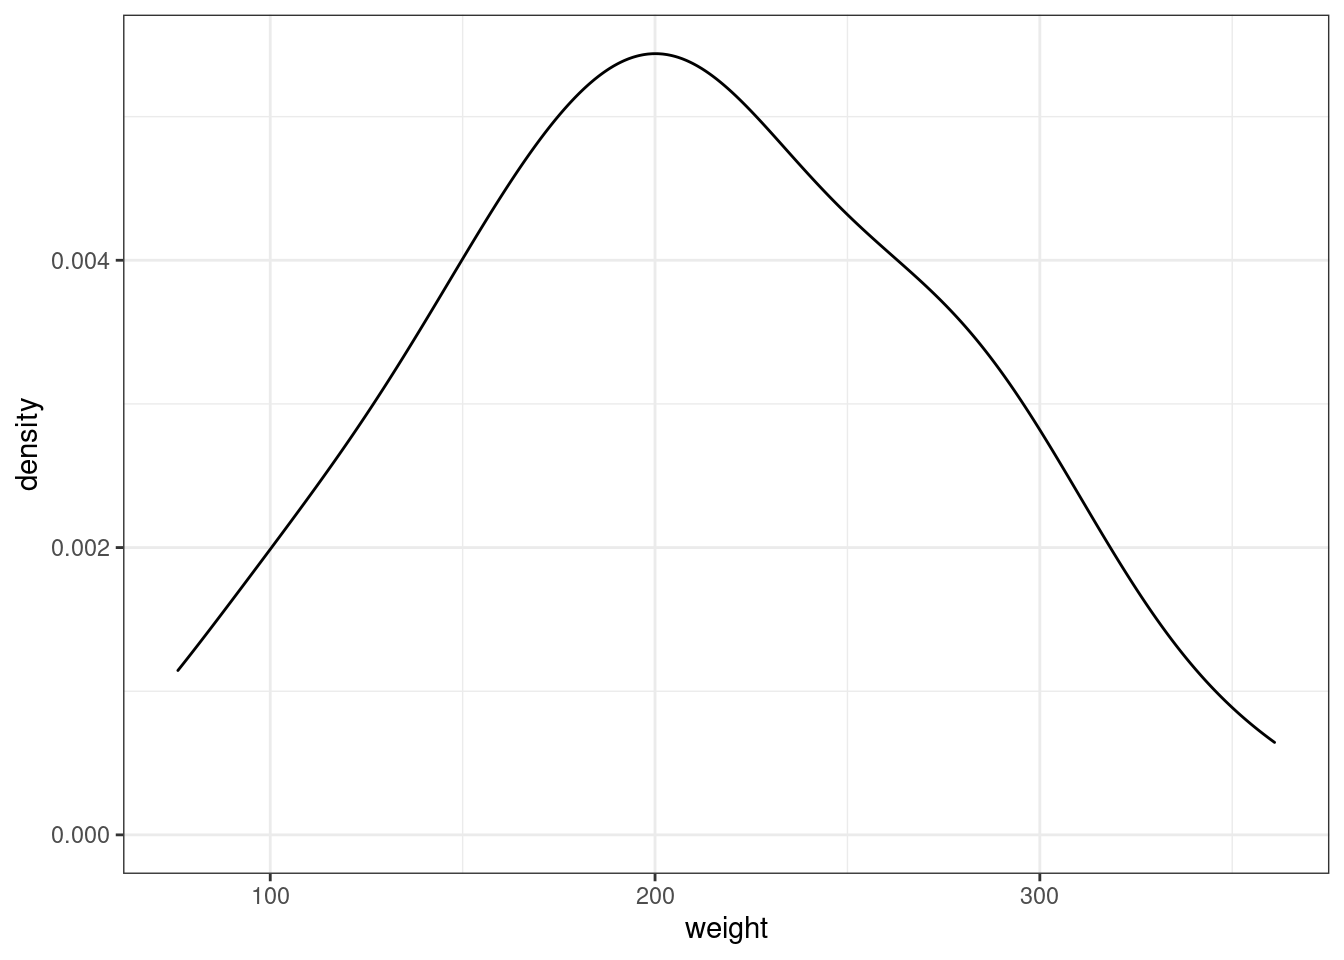
\includegraphics{da4l_files/figure-latex/unnamed-chunk-87-1.pdf}

Начнем с апостериорных параметров для наблюдений \(x_1, ... x_n\) со средним \(\mu_{data}\) известной дисперсией \(\sigma_{known}^2\)

\hypertarget{ux431ux430ux439ux435ux441ux43eux432ux441ux43aux438ux439-ux430ux43fux434ux435ux439ux442-ux43dux43eux440ux43cux430ux43bux44cux43dux43eux433ux43e-ux440ux430ux441ux43fux440ux435ux434ux435ux43bux435ux43dux438ux44f-ux432ux44bux431ux43eux440-ux438ux437-ux43dux435ux441ux43aux43eux43bux44cux43aux438ux445-ux43cux43eux434ux435ux43bux435ux439}{%
\subsection{Байесовский апдейт нормального распределения: выбор из нескольких моделей}\label{ux431ux430ux439ux435ux441ux43eux432ux441ux43aux438ux439-ux430ux43fux434ux435ux439ux442-ux43dux43eux440ux43cux430ux43bux44cux43dux43eux433ux43e-ux440ux430ux441ux43fux440ux435ux434ux435ux43bux435ux43dux438ux44f-ux432ux44bux431ux43eux440-ux438ux437-ux43dux435ux441ux43aux43eux43bux44cux43aux438ux445-ux43cux43eux434ux435ux43bux435ux439}}

Мы можем рассматривать эту задачу как выбор между несколькими моделями с разными средними:

\begin{Shaded}
\begin{Highlighting}[]
\FunctionTok{tibble}\NormalTok{(}\AttributeTok{x =} \FunctionTok{rep}\NormalTok{(}\DecValTok{1}\SpecialCharTok{:}\DecValTok{400}\NormalTok{, }\DecValTok{6}\NormalTok{),}
           \AttributeTok{density =} \FunctionTok{c}\NormalTok{(}\FunctionTok{dnorm}\NormalTok{(}\FunctionTok{unique}\NormalTok{(x), }\AttributeTok{mean =} \DecValTok{125}\NormalTok{, }\AttributeTok{sd =} \DecValTok{70}\NormalTok{),}
                       \FunctionTok{dnorm}\NormalTok{(}\FunctionTok{unique}\NormalTok{(x), }\AttributeTok{mean =} \DecValTok{150}\NormalTok{, }\AttributeTok{sd =} \DecValTok{70}\NormalTok{),}
                       \FunctionTok{dnorm}\NormalTok{(}\FunctionTok{unique}\NormalTok{(x), }\AttributeTok{mean =} \DecValTok{175}\NormalTok{, }\AttributeTok{sd =} \DecValTok{70}\NormalTok{),}
                       \FunctionTok{dnorm}\NormalTok{(}\FunctionTok{unique}\NormalTok{(x), }\AttributeTok{mean =} \DecValTok{200}\NormalTok{, }\AttributeTok{sd =} \DecValTok{70}\NormalTok{),}
                       \FunctionTok{dnorm}\NormalTok{(}\FunctionTok{unique}\NormalTok{(x), }\AttributeTok{mean =} \DecValTok{225}\NormalTok{, }\AttributeTok{sd =} \DecValTok{70}\NormalTok{),}
                       \FunctionTok{dnorm}\NormalTok{(}\FunctionTok{unique}\NormalTok{(x), }\AttributeTok{mean =} \DecValTok{250}\NormalTok{, }\AttributeTok{sd =} \DecValTok{70}\NormalTok{)),}
           \AttributeTok{dataset =} \FunctionTok{rep}\NormalTok{(}\DecValTok{1}\SpecialCharTok{:}\DecValTok{6}\NormalTok{, }\AttributeTok{each =} \DecValTok{400}\NormalTok{)) }\SpecialCharTok{\%\textgreater{}\%} 
  \FunctionTok{ggplot}\NormalTok{(}\FunctionTok{aes}\NormalTok{(x, density, }\AttributeTok{color =} \FunctionTok{factor}\NormalTok{(dataset)))}\SpecialCharTok{+}
  \FunctionTok{geom\_line}\NormalTok{()}
\end{Highlighting}
\end{Shaded}

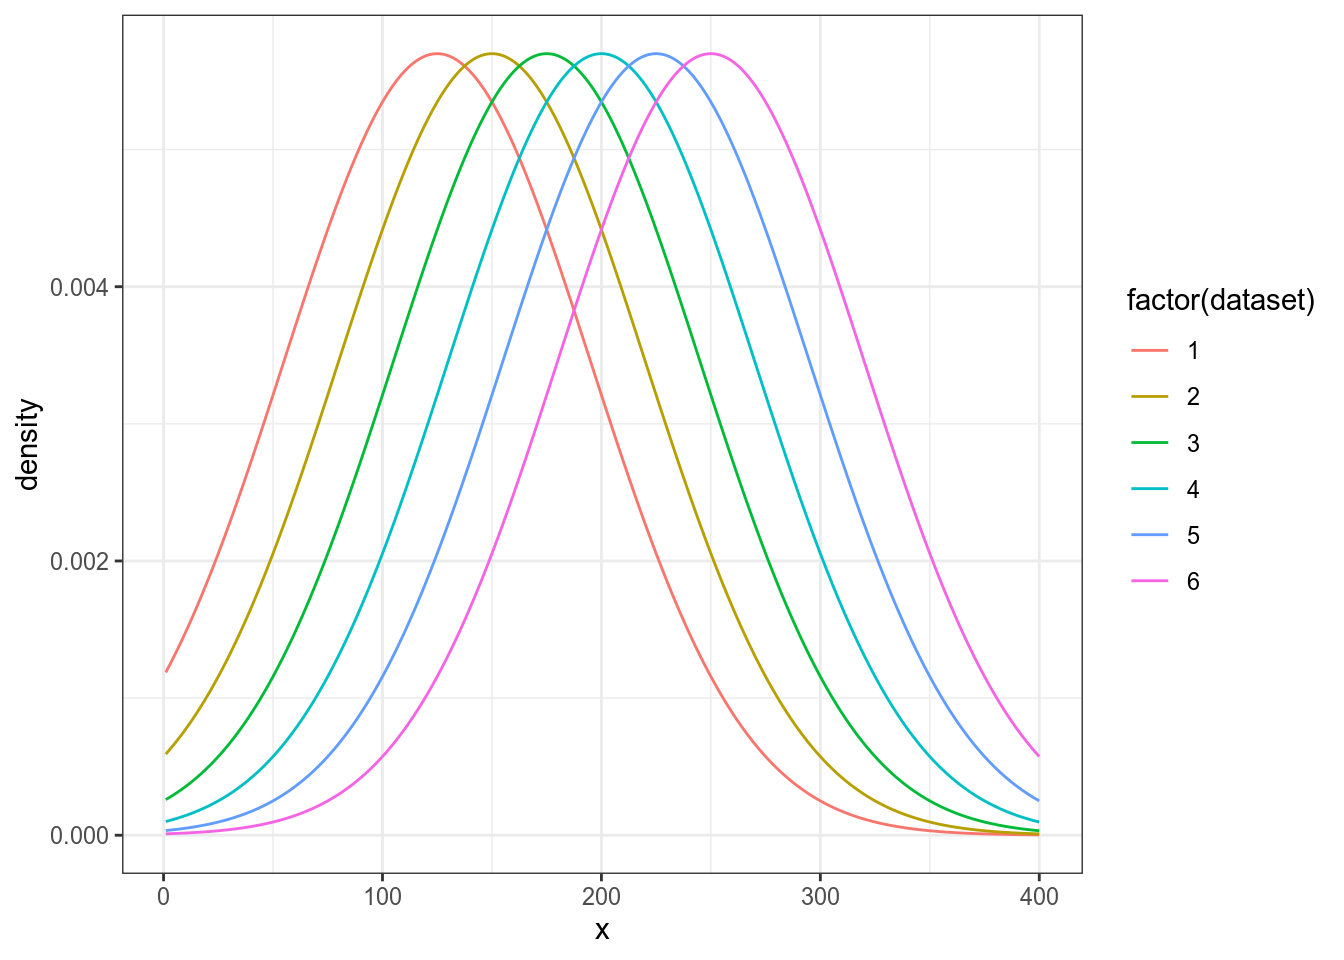
\includegraphics{da4l_files/figure-latex/unnamed-chunk-88-1.pdf}

Дальше мы можем точно так же апдейтить, как мы делали раньше:

\begin{Shaded}
\begin{Highlighting}[]
\FunctionTok{tibble}\NormalTok{(}\AttributeTok{mu =} \FunctionTok{seq}\NormalTok{(}\DecValTok{125}\NormalTok{, }\DecValTok{250}\NormalTok{, }\AttributeTok{by =} \DecValTok{25}\NormalTok{),}
           \AttributeTok{prior =} \DecValTok{1}\SpecialCharTok{/}\DecValTok{6}\NormalTok{,}
           \AttributeTok{likelihood =} \FunctionTok{c}\NormalTok{(}\FunctionTok{prod}\NormalTok{(}\FunctionTok{dnorm}\NormalTok{(chicks}\SpecialCharTok{$}\NormalTok{weight, }\AttributeTok{mean =} \DecValTok{125}\NormalTok{, }\AttributeTok{sd =} \DecValTok{70}\NormalTok{)),}
                          \FunctionTok{prod}\NormalTok{(}\FunctionTok{dnorm}\NormalTok{(chicks}\SpecialCharTok{$}\NormalTok{weight, }\AttributeTok{mean =} \DecValTok{150}\NormalTok{, }\AttributeTok{sd =} \DecValTok{70}\NormalTok{)),}
                          \FunctionTok{prod}\NormalTok{(}\FunctionTok{dnorm}\NormalTok{(chicks}\SpecialCharTok{$}\NormalTok{weight, }\AttributeTok{mean =} \DecValTok{175}\NormalTok{, }\AttributeTok{sd =} \DecValTok{70}\NormalTok{)),}
                          \FunctionTok{prod}\NormalTok{(}\FunctionTok{dnorm}\NormalTok{(chicks}\SpecialCharTok{$}\NormalTok{weight, }\AttributeTok{mean =} \DecValTok{200}\NormalTok{, }\AttributeTok{sd =} \DecValTok{70}\NormalTok{)),}
                          \FunctionTok{prod}\NormalTok{(}\FunctionTok{dnorm}\NormalTok{(chicks}\SpecialCharTok{$}\NormalTok{weight, }\AttributeTok{mean =} \DecValTok{225}\NormalTok{, }\AttributeTok{sd =} \DecValTok{70}\NormalTok{)),}
                          \FunctionTok{prod}\NormalTok{(}\FunctionTok{dnorm}\NormalTok{(chicks}\SpecialCharTok{$}\NormalTok{weight, }\AttributeTok{mean =} \DecValTok{250}\NormalTok{, }\AttributeTok{sd =} \DecValTok{70}\NormalTok{))),}
           \AttributeTok{product =}\NormalTok{ prior}\SpecialCharTok{*}\NormalTok{likelihood,}
           \AttributeTok{posterior =}\NormalTok{ product}\SpecialCharTok{/}\FunctionTok{sum}\NormalTok{(product)) }\OtherTok{{-}\textgreater{}}
\NormalTok{  results}
\NormalTok{results}
\end{Highlighting}
\end{Shaded}

\begin{verbatim}
# A tibble: 6 x 5
     mu prior likelihood   product posterior
  <dbl> <dbl>      <dbl>     <dbl>     <dbl>
1   125 0.167  2.06e-127 3.44e-128  2.39e-15
2   150 0.167  4.74e-120 7.90e-121  5.48e- 8
3   175 0.167  3.08e-115 5.13e-116  3.56e- 3
4   200 0.167  5.66e-113 9.43e-114  6.55e- 1
5   225 0.167  2.95e-113 4.91e-114  3.41e- 1
6   250 0.167  4.34e-116 7.23e-117  5.02e- 4
\end{verbatim}

\begin{Shaded}
\begin{Highlighting}[]
\NormalTok{results }\SpecialCharTok{\%\textgreater{}\%} 
  \FunctionTok{select}\NormalTok{(mu, prior, posterior) }\SpecialCharTok{\%\textgreater{}\%} 
  \FunctionTok{pivot\_longer}\NormalTok{(}\AttributeTok{names\_to =} \StringTok{"type"}\NormalTok{, }\AttributeTok{values\_to =} \StringTok{"probability"}\NormalTok{, prior}\SpecialCharTok{:}\NormalTok{posterior) }\SpecialCharTok{\%\textgreater{}\%} 
  \FunctionTok{ggplot}\NormalTok{(}\FunctionTok{aes}\NormalTok{(mu, probability, }\AttributeTok{color =}\NormalTok{ type))}\SpecialCharTok{+}
  \FunctionTok{geom\_point}\NormalTok{()}\SpecialCharTok{+}
  \FunctionTok{labs}\NormalTok{(}\AttributeTok{title =} \StringTok{"изменение вероятностей для каждой из моделей"}\NormalTok{,}
       \AttributeTok{x =} \StringTok{"μ"}\NormalTok{)}
\end{Highlighting}
\end{Shaded}

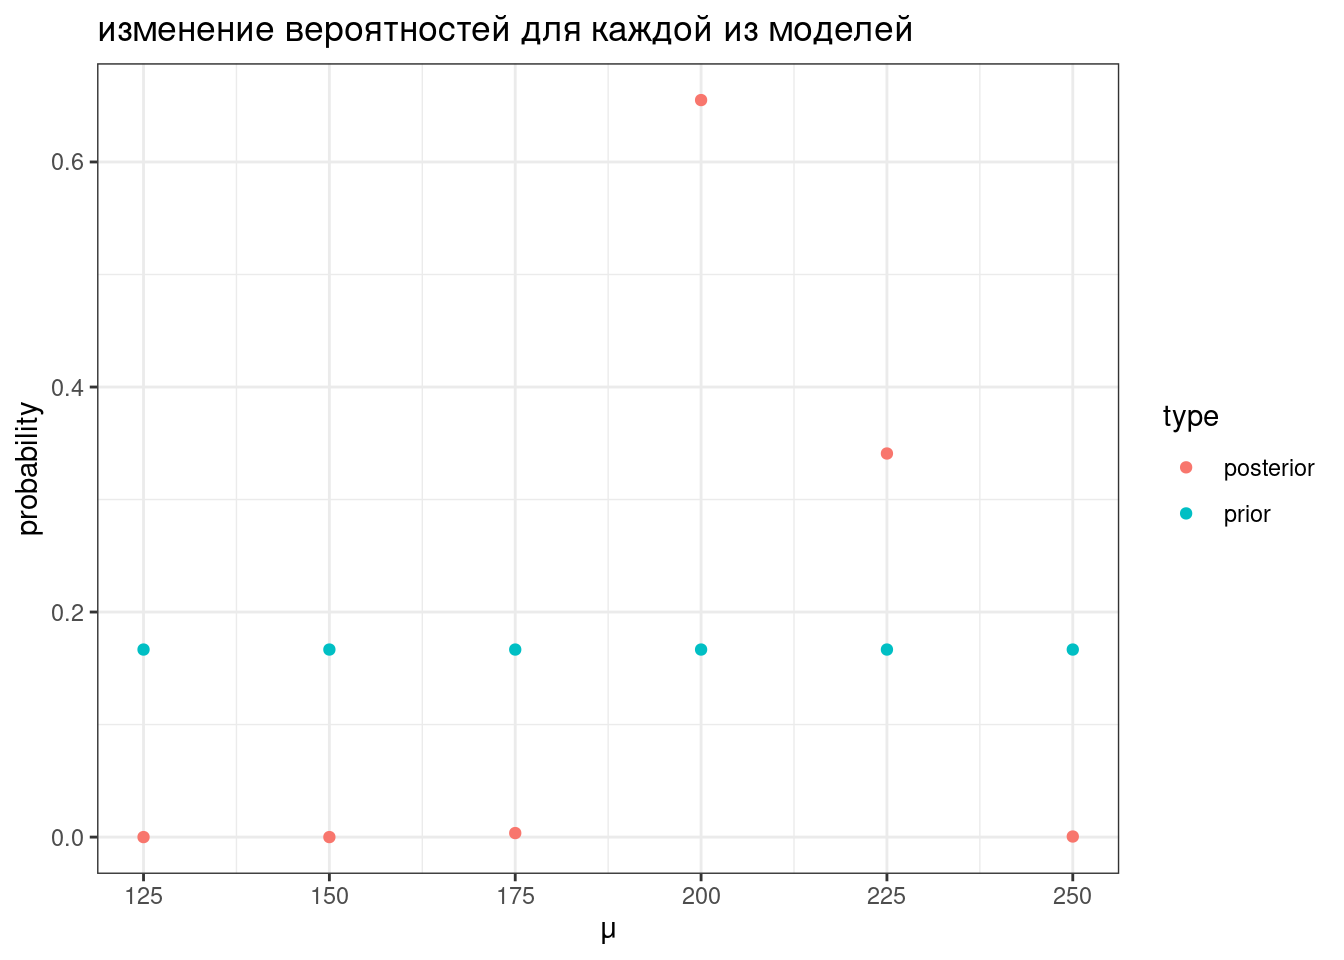
\includegraphics{da4l_files/figure-latex/unnamed-chunk-89-1.pdf}

\hypertarget{ux431ux430ux439ux435ux441ux43eux432ux441ux43aux438ux439-ux430ux43fux434ux435ux439ux442-ux43dux43eux440ux43cux430ux43bux44cux43dux43eux433ux43e-ux440ux430ux441ux43fux440ux435ux434ux435ux43bux435ux43dux438ux44f-ux43dux435ux43fux440ux435ux440ux44bux432ux43dux44bux439-ux432ux430ux440ux438ux430ux43dux442}{%
\subsection{Байесовский апдейт нормального распределения: непрерывный вариант}\label{ux431ux430ux439ux435ux441ux43eux432ux441ux43aux438ux439-ux430ux43fux434ux435ux439ux442-ux43dux43eux440ux43cux430ux43bux44cux43dux43eux433ux43e-ux440ux430ux441ux43fux440ux435ux434ux435ux43bux435ux43dux438ux44f-ux43dux435ux43fux440ux435ux440ux44bux432ux43dux44bux439-ux432ux430ux440ux438ux430ux43dux442}}

Во первых, нам понадобится некоторая мера, которая называется \emph{точность} (precision):

\[\tau = \frac{1}{\sigma^2}\]

\[\tau_{post} = \tau_{prior} + \tau_{data} \Rightarrow \sigma^2_{post} = \frac{1}{\tau_{post}}\]

\[\mu_{post} = \frac{\mu_{prior} \times \tau_{prior} + \mu_{data} \times \tau_{data}}{\tau_{post}}\]

Так что если нашим априорным распределением мы назовем нормальное распределение со средним около 180 и стандартным отклонением 90, то процесс байесовского апдейта будет выглядеть вот так:

\begin{Shaded}
\begin{Highlighting}[]
\NormalTok{sd\_prior }\OtherTok{\textless{}{-}} \DecValTok{90} 
\NormalTok{sd\_data }\OtherTok{\textless{}{-}} \FunctionTok{sd}\NormalTok{(chicks}\SpecialCharTok{$}\NormalTok{weight)}
\NormalTok{sd\_post }\OtherTok{\textless{}{-}} \DecValTok{1}\SpecialCharTok{/}\FunctionTok{sqrt}\NormalTok{(}\DecValTok{1}\SpecialCharTok{/}\NormalTok{sd\_prior}\SpecialCharTok{\^{}}\DecValTok{2} \SpecialCharTok{+} \DecValTok{1}\SpecialCharTok{/}\NormalTok{sd\_data}\SpecialCharTok{\^{}}\DecValTok{2}\NormalTok{)}
\NormalTok{mean\_prior }\OtherTok{\textless{}{-}} \DecValTok{180}
\NormalTok{mean\_data }\OtherTok{\textless{}{-}} \FunctionTok{mean}\NormalTok{(chicks}\SpecialCharTok{$}\NormalTok{weight)}
\NormalTok{mean\_post }\OtherTok{\textless{}{-}} \FunctionTok{weighted.mean}\NormalTok{(}\FunctionTok{c}\NormalTok{(mean\_prior, mean\_data), }\FunctionTok{c}\NormalTok{(}\DecValTok{1}\SpecialCharTok{/}\NormalTok{sd\_prior}\SpecialCharTok{\^{}}\DecValTok{2}\NormalTok{, }\DecValTok{1}\SpecialCharTok{/}\NormalTok{sd\_data}\SpecialCharTok{\^{}}\DecValTok{2}\NormalTok{))}

\NormalTok{chicks }\SpecialCharTok{\%\textgreater{}\%} 
  \FunctionTok{ggplot}\NormalTok{(}\FunctionTok{aes}\NormalTok{(weight)) }\SpecialCharTok{+}
  \FunctionTok{geom\_histogram}\NormalTok{(}\FunctionTok{aes}\NormalTok{(}\AttributeTok{y =}\NormalTok{ ..density..))}\SpecialCharTok{+}
  \FunctionTok{stat\_function}\NormalTok{(}\AttributeTok{fun =}\NormalTok{ dnorm, }\AttributeTok{args =} \FunctionTok{list}\NormalTok{(mean\_prior,  sd\_prior), }\AttributeTok{color =} \StringTok{"lightblue"}\NormalTok{)}\SpecialCharTok{+}
  \FunctionTok{stat\_function}\NormalTok{(}\AttributeTok{fun =}\NormalTok{ dnorm, }\AttributeTok{args =} \FunctionTok{list}\NormalTok{(mean\_post,  sd\_post), }\AttributeTok{color =} \StringTok{"red"}\NormalTok{)}
\end{Highlighting}
\end{Shaded}

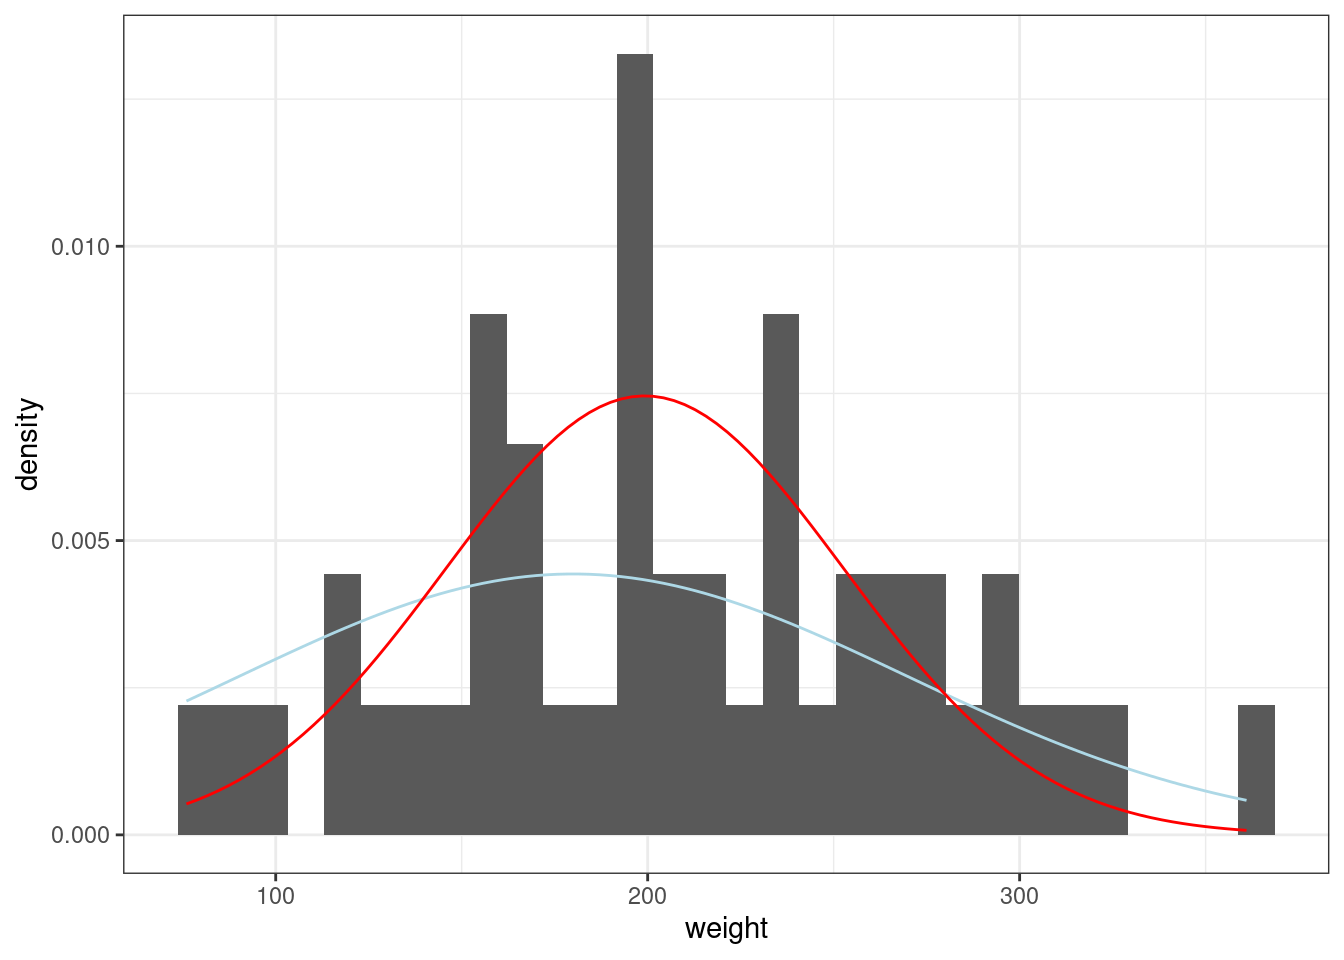
\includegraphics{da4l_files/figure-latex/unnamed-chunk-90-1.pdf}

\begin{Shaded}
\begin{Highlighting}[]
\NormalTok{shiny}\SpecialCharTok{::}\FunctionTok{runGitHub}\NormalTok{(}\StringTok{"agricolamz/bayes\_for\_normal\_app"}\NormalTok{) }
\end{Highlighting}
\end{Shaded}

\begin{rmdtask}
В работе {[}@coretta2016{]} собраны
\href{https://raw.githubusercontent.com/agricolamz/2021_da4l/master/data/Coretta_2017_icelandic.csv}{данные}
длительности исландских гласных. Отфильтруйте данные, произнесенные
носителем \texttt{tt01} (переменная \texttt{speaker}), произведите
байесовский апдейт данных, моделируя длительность гласных (переменная
\texttt{vowel.dur}) нормальным распределением и постройте график. В
качестве априорного распределения используйте нормальное распределение
со средним 87 и стандартным отклонением 25.
\end{rmdtask}

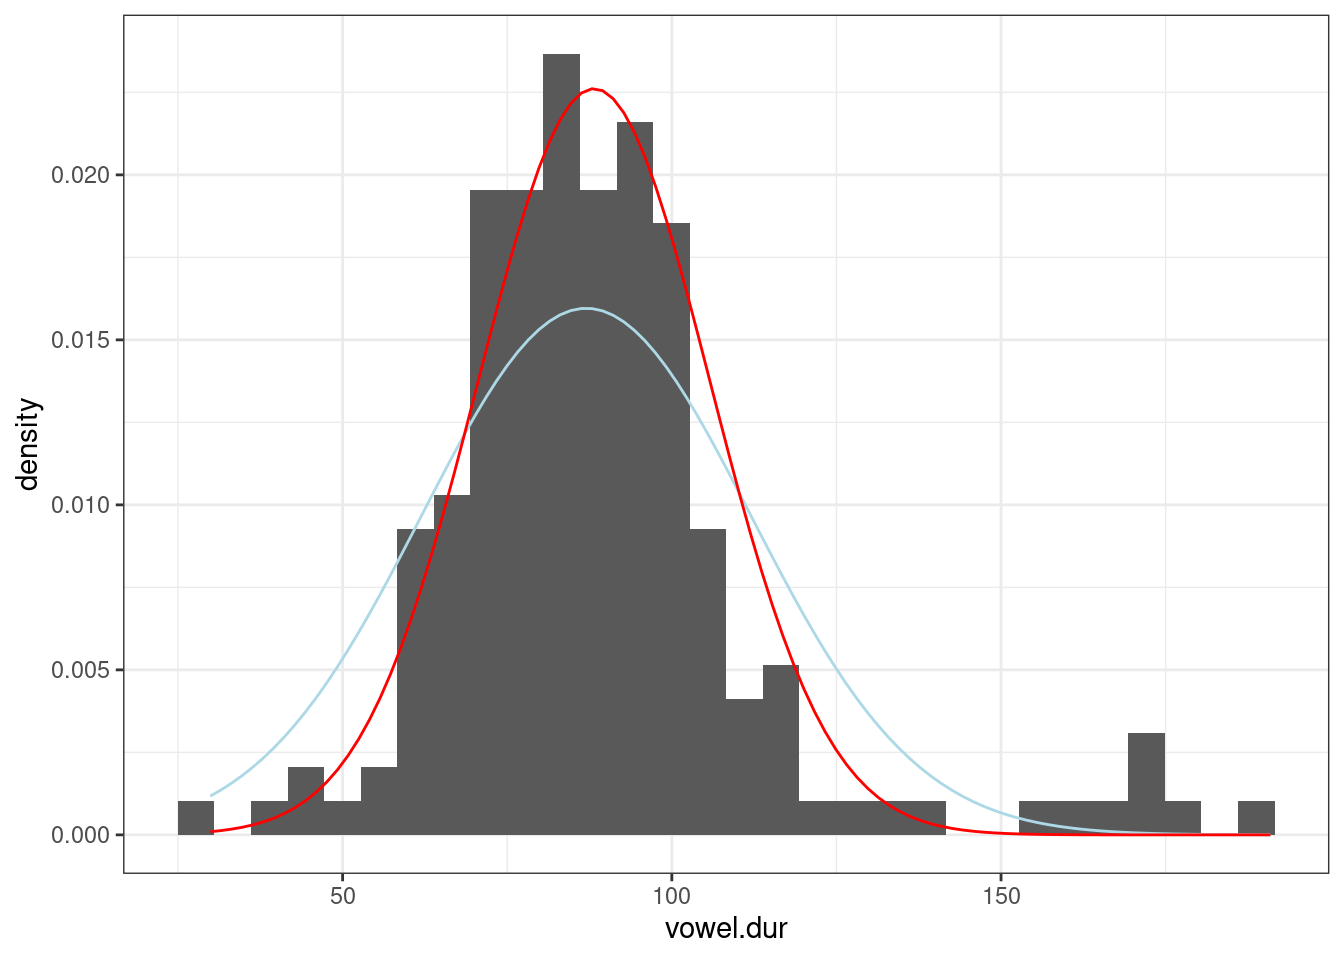
\includegraphics{da4l_files/figure-latex/unnamed-chunk-93-1.pdf}

\hypertarget{ux447ux442ux43e-ux43fux43eux447ux438ux442ux430ux442ux44c-1}{%
\subsection{Что почитать?}\label{ux447ux442ux43e-ux43fux43eux447ux438ux442ux430ux442ux44c-1}}

\begin{itemize}
\tightlist
\item
  \href{https://www.cs.ubc.ca/~murphyk/Papers/bayesGauss.pdf}{Murphy K. P. (2007) Conjugate Bayesian analysis of the Gaussian distribution}
\item
  \href{https://people.eecs.berkeley.edu/~jordan/courses/260-spring10/lectures/lecture5.pdf}{Jordan M. I. (2010) The Conjugate Prior for the Normal Distribution}
\item
  раздел 2.5 в Gelman A. et. al (2014) Bayesian Data Analysis
\end{itemize}

\hypertarget{ux434ux440ux443ux433ux438ux435-ux440ux430ux441ux43fux440ux435ux434ux435ux43bux435ux43dux438ux44f}{%
\section{Другие распределения}\label{ux434ux440ux443ux433ux438ux435-ux440ux430ux441ux43fux440ux435ux434ux435ux43bux435ux43dux438ux44f}}

Мы обсудили биномиальные и нормальнораспределенные данные. Так случилось, что для них есть короткий путь сделать байесовский апдейт, не применяя формулы байеса. И нам так повезло, что связки априорного/апосториорного распределений и функции правдоподобия такие простые:

\begin{itemize}
\tightlist
\item
  априорного/апосториорного распределены как бета распределение, значит функция правдоподобия -- биномиальное распределение
\item
  если мы моделируем данные при помощи нормального распределения, то все три распределения (априорное, функция правдопдобия и апосториорное) -- нормальные.
\end{itemize}

Такие отношения между распределениями называют сопряженными (conjugate). В результате для разных семейств функции правдоподобия существует список соответствующих сопряженных априорных распределений (conjugate prior), который можно найти, например, \href{https://en.wikipedia.org/wiki/Conjugate_prior}{здесь}.

В более случаях используется (а на самом деле почти всегда) Марковские цепи Монте-Карло (MCMC).

\hypertarget{ux432ux43eux43fux440ux43eux441ux44b-ux43a-ux430ux43fux43eux441ux442ux435ux440ux438ux43eux440ux43dux43eux43cux443-ux440ux430ux441ux43fux440ux435ux434ux435ux43bux435ux43dux438ux44e}{%
\section{Вопросы к апостериорному распределению}\label{ux432ux43eux43fux440ux43eux441ux44b-ux43a-ux430ux43fux43eux441ux442ux435ux440ux438ux43eux440ux43dux43eux43cux443-ux440ux430ux441ux43fux440ux435ux434ux435ux43bux435ux43dux438ux44e}}

\begin{quote}
A frequentist uses impeccable logic to answer the wrong question, while a Bayesian answers the right question by making assumptions that nobody can fully believe in. (P. G. Hammer)
\end{quote}

\begin{enumerate}
\def\labelenumi{\arabic{enumi})}
\tightlist
\item
  попытка оценить параметр θ и/или какой-нибудь интервал, в котором он лежит.

  \begin{itemize}
  \tightlist
  \item
    среднее апостериорного распределения (mean of the posterior estimation, MAP)
  \item
    максимум апостериорного распределения (maximum a posteriori estimation, MAP)
  \item
    байесовский доверительный интервал
  \end{itemize}
\item
  ответить на вопросы вроде

  \begin{itemize}
  \tightlist
  \item
    какова вероятность, что значение θ больше некоторого значения \(x\)?
  \item
    какова вероятность, что значение θ лежит в интервале \([x; y]\)?
  \item
    и т. п.
  \end{itemize}
\item
  Выборки из апостериорного распределения (Posterior simulation):

  \begin{itemize}
  \tightlist
  \item
    симулируйте большую выборку из апостериорного распределения;
  \item
    используйте полученную выборку для статистического вывода.
  \end{itemize}
\end{enumerate}

Допустим, мы получили апостериорное бета распределение с параметрами 20 и 70. Какова вероятность наблюдать значения больше 0.3?

\begin{Shaded}
\begin{Highlighting}[]
\NormalTok{posterior\_simulation }\OtherTok{\textless{}{-}} \FunctionTok{rbeta}\NormalTok{(}\AttributeTok{n =} \DecValTok{10000}\NormalTok{, }\AttributeTok{shape1 =} \DecValTok{20}\NormalTok{, }\AttributeTok{shape2 =} \DecValTok{70}\NormalTok{)}
\FunctionTok{sum}\NormalTok{(posterior\_simulation }\SpecialCharTok{\textgreater{}} \FloatTok{0.3}\NormalTok{)}\SpecialCharTok{/}\DecValTok{10000}
\end{Highlighting}
\end{Shaded}

\begin{verbatim}
[1] 0.0424
\end{verbatim}

И это не p-value! Это настоящие вероятности!

\hypertarget{ux431ux430ux439ux435ux441ux43eux432ux441ux43aux438ux439-ux434ux43eux432ux435ux440ux438ux442ux435ux43bux44cux43dux44bux439-ux438ux43dux442ux435ux440ux432ux430ux43b}{%
\chapter{Байесовский доверительный интервал}\label{ux431ux430ux439ux435ux441ux43eux432ux441ux43aux438ux439-ux434ux43eux432ux435ux440ux438ux442ux435ux43bux44cux43dux44bux439-ux438ux43dux442ux435ux440ux432ux430ux43b}}

Рассмотрим простенькую задачу, которую мы видели раньше:

\begin{rmdtask}
Немного упрощая данные из статьи {[}@rosenbach03: 394{]}, можно сказать
что носители британского английского предпочитают \emph{s}-генитив
(90\%) \emph{of}-генитиву (10\%). Проведите байесовский апдейт, если Вы
наблюдаете в интервью британского актера из 120 контекстов 92
\emph{s}-генитивов. Априорное распределение берите соразмерное данным.
Ответ округлите до трёх или менее знаков после запятой.
\end{rmdtask}

\begin{Shaded}
\begin{Highlighting}[]
\FunctionTok{tibble}\NormalTok{(}\AttributeTok{x =} \FunctionTok{seq}\NormalTok{(}\DecValTok{0}\NormalTok{, }\DecValTok{1}\NormalTok{, }\AttributeTok{by =} \FloatTok{0.001}\NormalTok{),}
       \AttributeTok{y =} \FunctionTok{dbeta}\NormalTok{(x, }\DecValTok{108}\SpecialCharTok{+}\DecValTok{92}\NormalTok{, }\DecValTok{12}\SpecialCharTok{+}\DecValTok{28}\NormalTok{)) }\SpecialCharTok{\%\textgreater{}\%} 
  \FunctionTok{ggplot}\NormalTok{(}\FunctionTok{aes}\NormalTok{(x, y))}\SpecialCharTok{+}
  \FunctionTok{geom\_line}\NormalTok{()}
\end{Highlighting}
\end{Shaded}

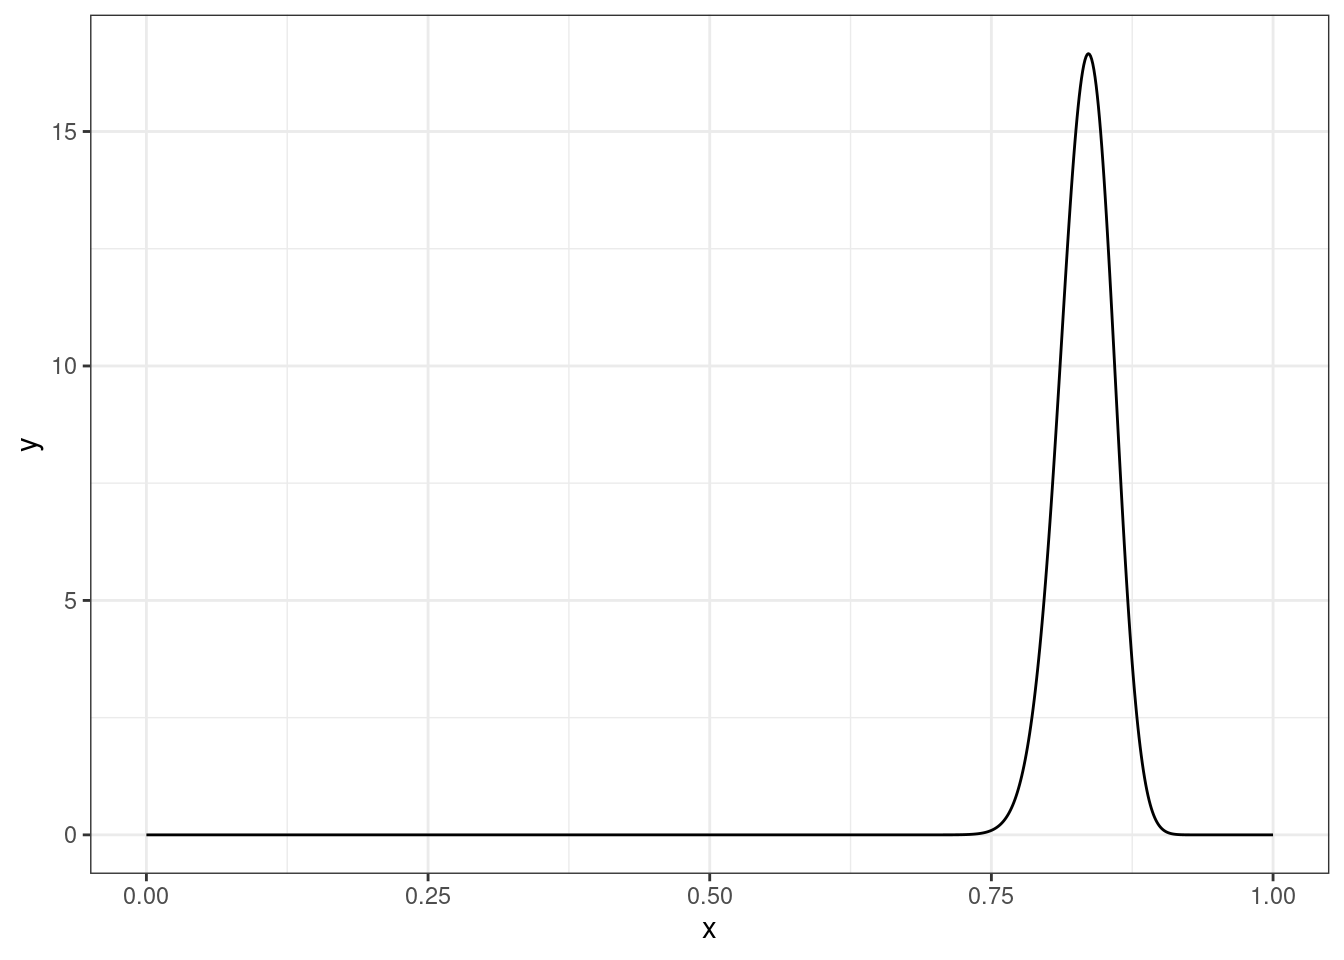
\includegraphics{da4l_files/figure-latex/unnamed-chunk-96-1.pdf}

\hypertarget{ux444ux440ux435ux43aux432ux435ux43dux442ux438ux441ux442ux43aux438ux439-ux434ux43eux432ux435ux440ux438ux442ux435ux43bux44cux43dux44bux439-ux438ux43dux442ux435ux440ux432ux430ux43b}{%
\section{Фреквентисткий доверительный интервал}\label{ux444ux440ux435ux43aux432ux435ux43dux442ux438ux441ux442ux43aux438ux439-ux434ux43eux432ux435ux440ux438ux442ux435ux43bux44cux43dux44bux439-ux438ux43dux442ux435ux440ux432ux430ux43b}}

Фреквентистский доверительный интервал (по-английски confidence interval) основан на правиле трех сигм нормального распределения:

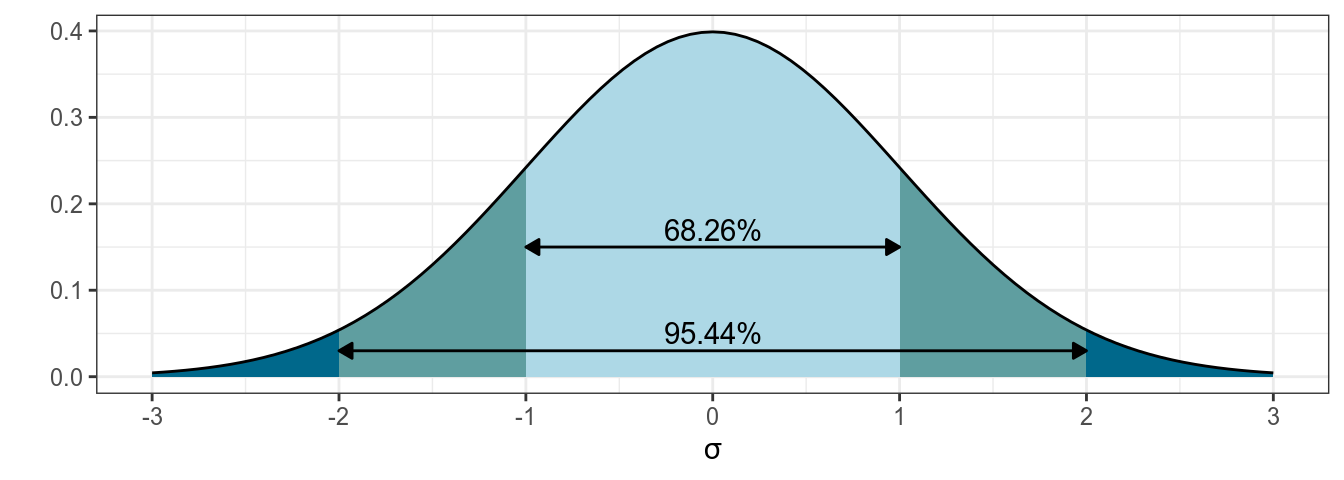
\includegraphics{da4l_files/figure-latex/unnamed-chunk-97-1.pdf}

\textbf{z-score}:

\begin{itemize}
\tightlist
\item
  95\% данных находится в 1.96 стандартных отклонений
\item
  99\% данных находится в 2.58 стандартных отклонений
\end{itemize}

Доверительный интервал:

\begin{itemize}
\tightlist
\item
  предположим, что данные генеральной совокупности нормально распределены
\item
  тогда доверительные интервалы выборок взятых из генеральной совокупности будут \href{https://rpsychologist.com/d3/CI/}{покрывать среднее генеральной совокупности}
\end{itemize}

\[\bar{x} \pm z \times \frac{\sigma}{\sqrt{n}}\text{, где } z \text{ — это центральная } 1 - \frac{\alpha}{2} \text{ часть данных}\]

Распространение этой логики на биномиальные данные называется интервал Вальда:

\[\bar{x} = \theta; \sigma = \sqrt{\frac{\theta\times(1-\theta)}{n}}\]

Тогда интервал Вальда:

\[\theta \pm  z\times\sqrt{\frac{\theta\times(1-\theta)} {n}}\]

Есть только одна проблема: работает он плохо. Его аналоги перечислены в других работ:

\begin{itemize}
\tightlist
\item
  assymptotic method with continuity correction
\item
  Wilson score
\item
  Wilson Score method with continuity correction
\item
  Jeffreys interval
\item
  Clopper--Pearson interval (default in R \texttt{binom.test()})
\item
  Agresti--Coull interval
\item
  \ldots{} см. пакет \texttt{binom}
\end{itemize}

\begin{Shaded}
\begin{Highlighting}[]
\NormalTok{low\_ci }\OtherTok{\textless{}{-}} \FunctionTok{binom.test}\NormalTok{(}\AttributeTok{x =} \DecValTok{108}\SpecialCharTok{+}\DecValTok{92}\NormalTok{, }\AttributeTok{n =} \DecValTok{108}\SpecialCharTok{+}\DecValTok{92}\SpecialCharTok{+}\DecValTok{12}\SpecialCharTok{+}\DecValTok{28}\NormalTok{)}\SpecialCharTok{$}\NormalTok{conf.int[}\DecValTok{1}\NormalTok{]}
\NormalTok{up\_ci }\OtherTok{\textless{}{-}}  \FunctionTok{binom.test}\NormalTok{(}\AttributeTok{x =} \DecValTok{108}\SpecialCharTok{+}\DecValTok{92}\NormalTok{, }\AttributeTok{n =} \DecValTok{108}\SpecialCharTok{+}\DecValTok{92}\SpecialCharTok{+}\DecValTok{12}\SpecialCharTok{+}\DecValTok{28}\NormalTok{)}\SpecialCharTok{$}\NormalTok{conf.int[}\DecValTok{2}\NormalTok{]}

\FunctionTok{tibble}\NormalTok{(}\AttributeTok{x =} \FunctionTok{seq}\NormalTok{(}\DecValTok{0}\NormalTok{, }\DecValTok{1}\NormalTok{, }\AttributeTok{by =} \FloatTok{0.001}\NormalTok{),}
       \AttributeTok{y =} \FunctionTok{dbeta}\NormalTok{(x, }\DecValTok{108}\SpecialCharTok{+}\DecValTok{92}\NormalTok{, }\DecValTok{12}\SpecialCharTok{+}\DecValTok{28}\NormalTok{)) }\SpecialCharTok{\%\textgreater{}\%} 
  \FunctionTok{ggplot}\NormalTok{(}\FunctionTok{aes}\NormalTok{(x, y))}\SpecialCharTok{+}
  \FunctionTok{geom\_line}\NormalTok{()}\SpecialCharTok{+}
  \FunctionTok{annotate}\NormalTok{(}\AttributeTok{geom =} \StringTok{"errorbar"}\NormalTok{, }\AttributeTok{y =} \DecValTok{0}\NormalTok{, }\AttributeTok{xmin =}\NormalTok{ low\_ci, }\AttributeTok{xmax =}\NormalTok{ up\_ci, }\AttributeTok{color =} \StringTok{"red"}\NormalTok{)}\SpecialCharTok{+}
  \FunctionTok{labs}\NormalTok{(}\AttributeTok{title =} \StringTok{"Апостериорное распределение"}\NormalTok{,}
       \AttributeTok{subtitle =} \StringTok{"красным фреквентисткий 95\% доверительный интервал"}\NormalTok{,}
       \AttributeTok{x =} \StringTok{""}\NormalTok{, }\AttributeTok{y =} \StringTok{""}\NormalTok{)}
\end{Highlighting}
\end{Shaded}

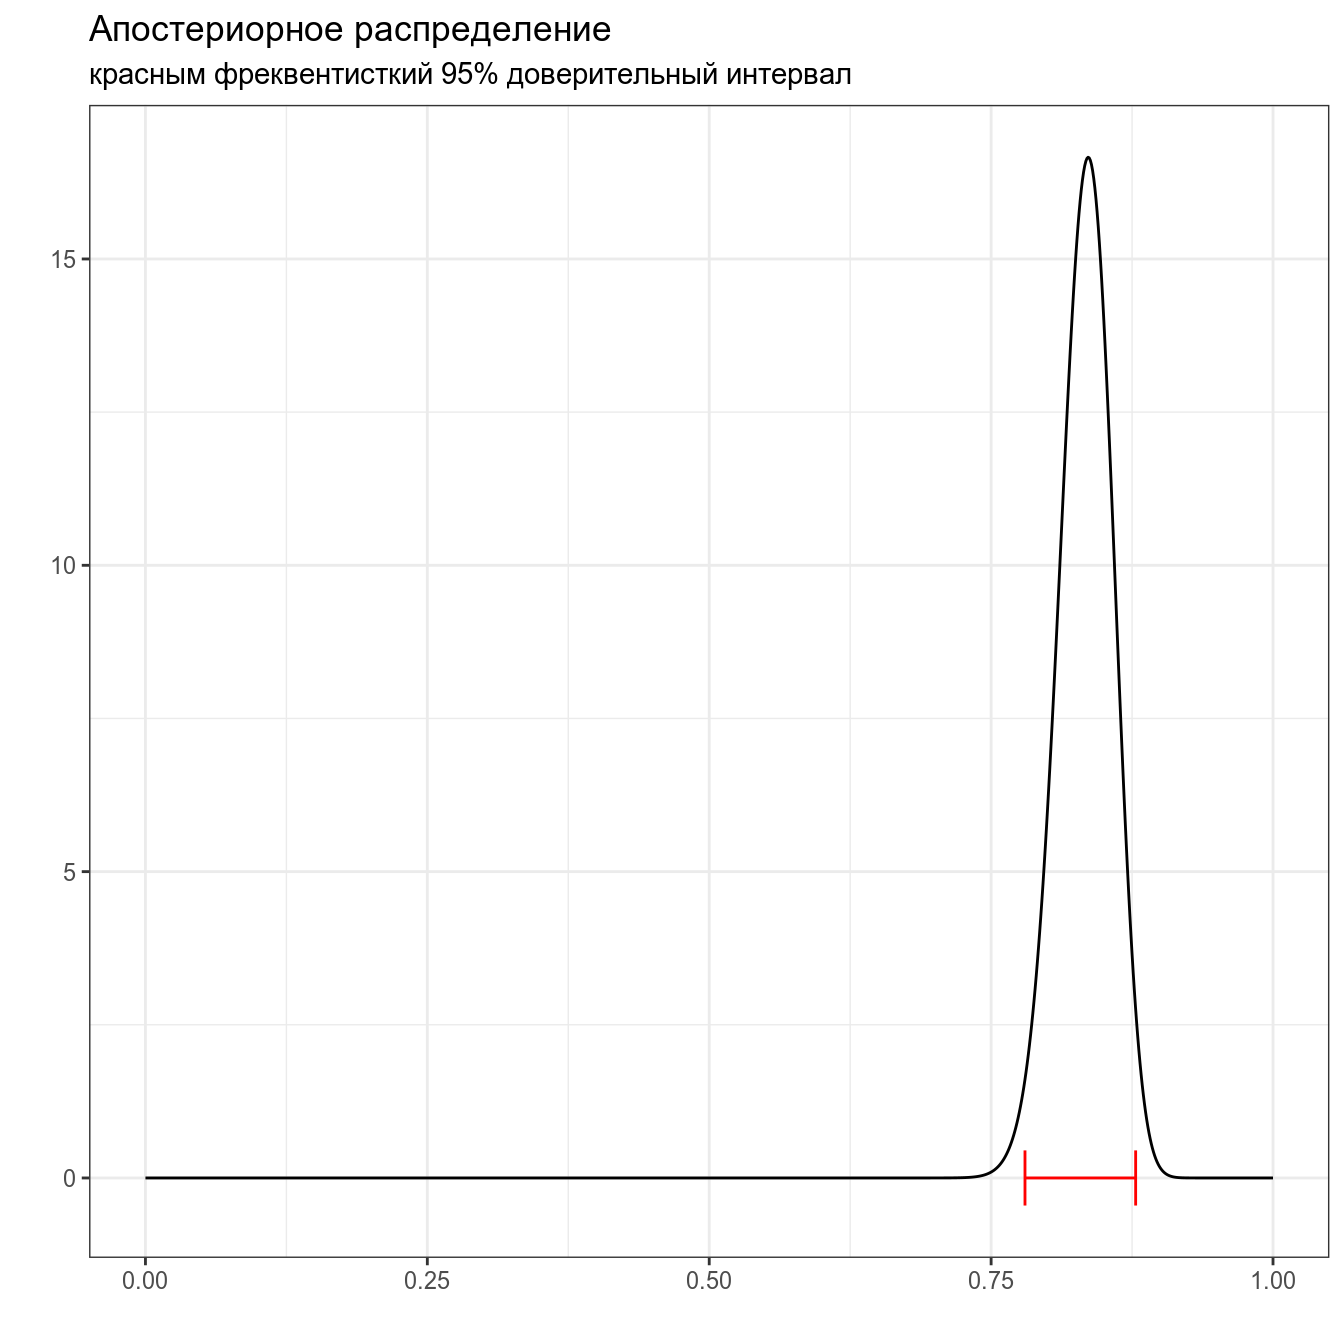
\includegraphics{da4l_files/figure-latex/unnamed-chunk-98-1.pdf}

В базовом пакете функция \texttt{binom.test()} не позволяет выбирать тип доверительного интервала. \texttt{ci.method\ =\ "Clopper-Pearson"} возможна, если включить библиотеку \texttt{mosaic}.

\hypertarget{ux431ux430ux439ux435ux441ux43eux432ux441ux43aux438ux439-ux434ux43eux432ux435ux440ux438ux442ux435ux43bux44cux43dux44bux439-ux438ux43dux442ux435ux440ux432ux430ux43b-1}{%
\section{Байесовский доверительный интервал}\label{ux431ux430ux439ux435ux441ux43eux432ux441ux43aux438ux439-ux434ux43eux432ux435ux440ux438ux442ux435ux43bux44cux43dux44bux439-ux438ux43dux442ux435ux440ux432ux430ux43b-1}}

Байесовский доверительный \((100-k)\)-\% интервал (по-английски credible interval) --- это интервал \([\frac{k}{2}, 1-\frac{k}{2}]\) от апостериорного распределения.

\begin{Shaded}
\begin{Highlighting}[]
\NormalTok{low\_ci }\OtherTok{\textless{}{-}} \FunctionTok{binom.test}\NormalTok{(}\AttributeTok{x =} \DecValTok{108}\SpecialCharTok{+}\DecValTok{92}\NormalTok{, }\AttributeTok{n =} \DecValTok{108}\SpecialCharTok{+}\DecValTok{92}\SpecialCharTok{+}\DecValTok{12}\SpecialCharTok{+}\DecValTok{28}\NormalTok{)}\SpecialCharTok{$}\NormalTok{conf.int[}\DecValTok{1}\NormalTok{]}
\NormalTok{up\_ci }\OtherTok{\textless{}{-}}  \FunctionTok{binom.test}\NormalTok{(}\AttributeTok{x =} \DecValTok{108}\SpecialCharTok{+}\DecValTok{92}\NormalTok{, }\AttributeTok{n =} \DecValTok{108}\SpecialCharTok{+}\DecValTok{92}\SpecialCharTok{+}\DecValTok{12}\SpecialCharTok{+}\DecValTok{28}\NormalTok{)}\SpecialCharTok{$}\NormalTok{conf.int[}\DecValTok{2}\NormalTok{]}

\NormalTok{cred\_int\_l }\OtherTok{\textless{}{-}} \FunctionTok{qbeta}\NormalTok{(}\FloatTok{0.025}\NormalTok{, }\DecValTok{108}\SpecialCharTok{+}\DecValTok{92}\NormalTok{, }\DecValTok{12}\SpecialCharTok{+}\DecValTok{28}\NormalTok{)}
\NormalTok{cred\_int\_h }\OtherTok{\textless{}{-}} \FunctionTok{qbeta}\NormalTok{(}\FloatTok{0.975}\NormalTok{, }\DecValTok{108}\SpecialCharTok{+}\DecValTok{92}\NormalTok{, }\DecValTok{12}\SpecialCharTok{+}\DecValTok{28}\NormalTok{)}

\FunctionTok{tibble}\NormalTok{(}\AttributeTok{x =} \FunctionTok{seq}\NormalTok{(}\DecValTok{0}\NormalTok{, }\DecValTok{1}\NormalTok{, }\AttributeTok{by =} \FloatTok{0.001}\NormalTok{),}
       \AttributeTok{y =} \FunctionTok{dbeta}\NormalTok{(x, }\DecValTok{108}\SpecialCharTok{+}\DecValTok{92}\NormalTok{, }\DecValTok{12}\SpecialCharTok{+}\DecValTok{28}\NormalTok{)) }\SpecialCharTok{\%\textgreater{}\%} 
  \FunctionTok{ggplot}\NormalTok{(}\FunctionTok{aes}\NormalTok{(x, y))}\SpecialCharTok{+}
  \FunctionTok{geom\_line}\NormalTok{()}\SpecialCharTok{+}
  \FunctionTok{annotate}\NormalTok{(}\AttributeTok{geom =} \StringTok{"errorbar"}\NormalTok{, }\AttributeTok{y =} \DecValTok{0}\NormalTok{, }\AttributeTok{xmin =}\NormalTok{ low\_ci, }\AttributeTok{xmax =}\NormalTok{ up\_ci, }\AttributeTok{color =} \StringTok{"red"}\NormalTok{)}\SpecialCharTok{+}
  \FunctionTok{annotate}\NormalTok{(}\AttributeTok{geom =} \StringTok{"errorbar"}\NormalTok{, }\AttributeTok{y =} \SpecialCharTok{{-}}\DecValTok{1}\NormalTok{, }\AttributeTok{xmin =}\NormalTok{ cred\_int\_l, }\AttributeTok{xmax =}\NormalTok{ cred\_int\_h, }\AttributeTok{color =} \StringTok{"lightblue"}\NormalTok{)}\SpecialCharTok{+}
  \FunctionTok{labs}\NormalTok{(}\AttributeTok{title =} \StringTok{"Апостериорное распределение"}\NormalTok{,}
       \AttributeTok{subtitle =} \StringTok{"красным фреквентисткий 95\% доверительный интервал}\SpecialCharTok{\textbackslash{}n}\StringTok{синим байесовский 95\% доверительный интервал"}\NormalTok{,}
       \AttributeTok{x =} \StringTok{""}\NormalTok{, }\AttributeTok{y =} \StringTok{""}\NormalTok{)}
\end{Highlighting}
\end{Shaded}

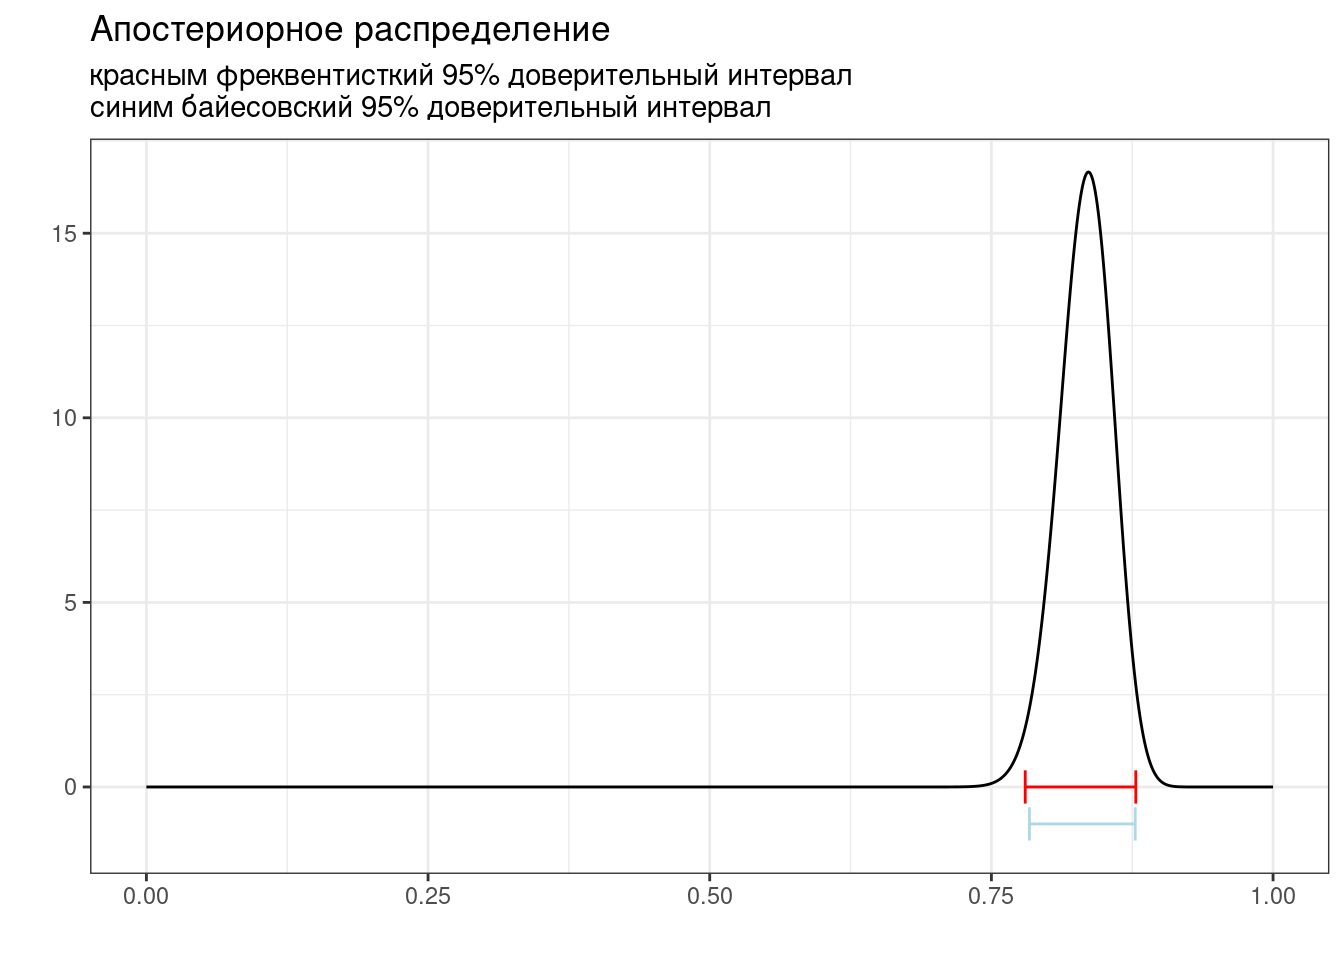
\includegraphics{da4l_files/figure-latex/unnamed-chunk-99-1.pdf}

\begin{rmdtask}
В работе {[}@coretta2016{]} собраны
\href{https://raw.githubusercontent.com/agricolamz/2021_da4l/master/data/Coretta_2017_icelandic.csv}{данные}
длительности исландских гласных. Отфильтруйте данные, произнесенные
носителем \texttt{tt01} (переменная \texttt{speaker}), произведите
байесовский апдейт данных, моделируя длительность гласных (переменная
\texttt{vowel.dur}) нормальным распределением и постройте график. На
графике отобразите 80\% байесовский доверительный интервал (при
построении интервала я использовал аргумент \texttt{width\ =\ 0.001}). В
качестве априорного распределения используйте нормальное распределение
со средним 87 и стандартным отклонением 25.
\end{rmdtask}

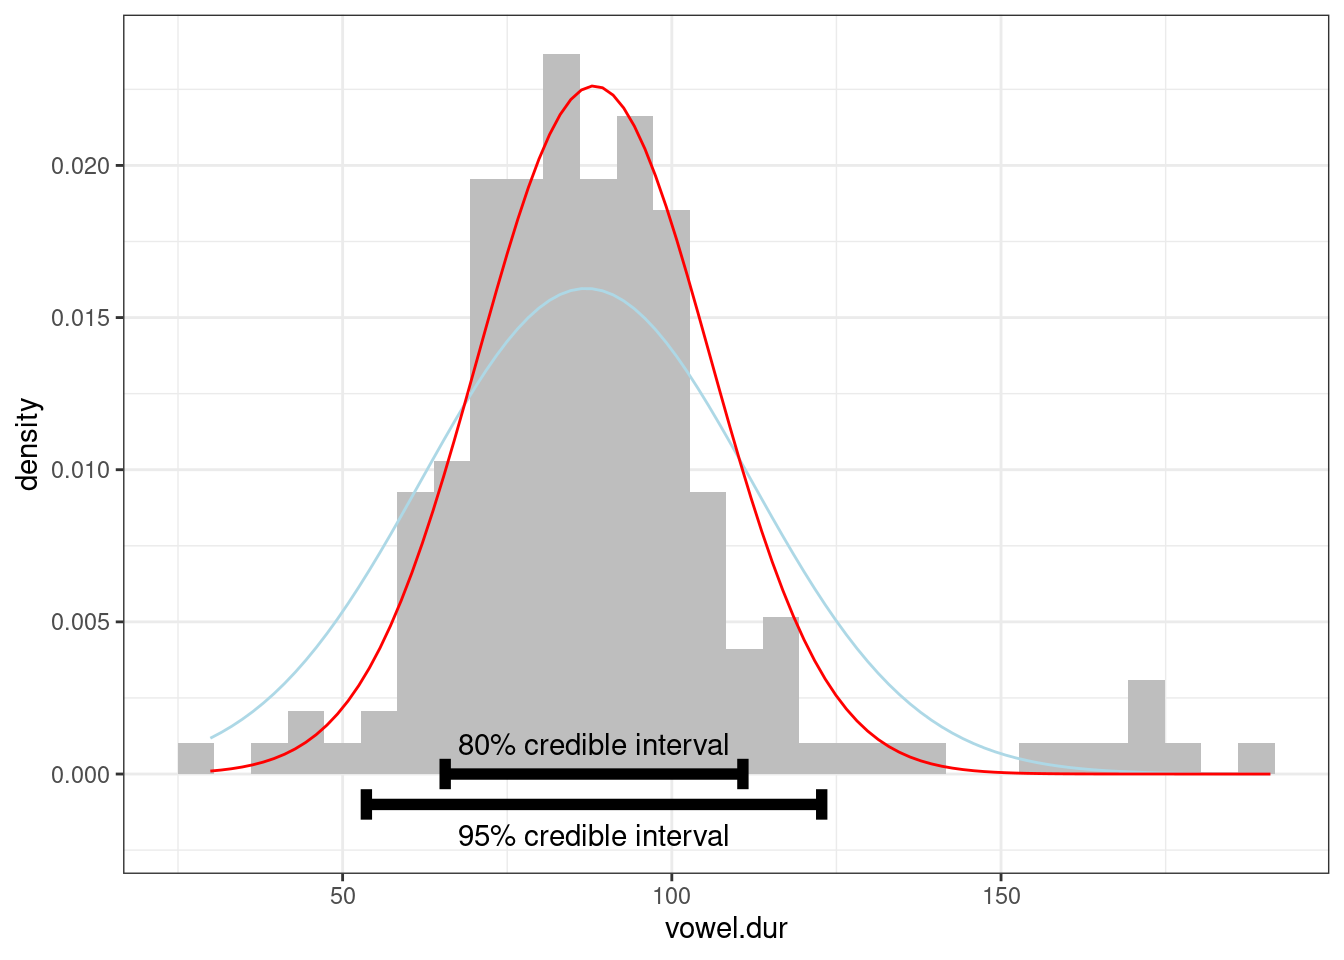
\includegraphics{da4l_files/figure-latex/unnamed-chunk-101-1.pdf}

\hypertarget{ux43aux43eux44dux444ux444ux438ux446ux438ux435ux43dux442-ux431ux430ux439ux435ux441ux430}{%
\chapter{Коэффициент Байеса}\label{ux43aux43eux44dux444ux444ux438ux446ux438ux435ux43dux442-ux431ux430ux439ux435ux441ux430}}

\hypertarget{ux43aux43eux44dux444ux444ux438ux446ux438ux435ux43dux442-ux431ux430ux439ux435ux441ux430-1}{%
\section{Коэффициент Байеса}\label{ux43aux43eux44dux444ux444ux438ux446ux438ux435ux43dux442-ux431ux430ux439ux435ux441ux430-1}}

\begin{Shaded}
\begin{Highlighting}[]
\FunctionTok{library}\NormalTok{(tidyverse)}
\end{Highlighting}
\end{Shaded}

В прошлой лекции мы обсуждали значения правдоподобия. Важно понимать, что само по себе значение правдоподобия бессмысленно, оно важно для сравнения со значениями правдоподобия разных моделей. Представим, что мы пытаемся выбрать между двумя моделями:

\begin{itemize}
\tightlist
\item
  \(H_1 = X \sim \ln\mathcal{N}(\mu = 3,\, \sigma^{2}= 0.37)\)
\item
  \(H_2 = X \sim \ln\mathcal{N}(\mu = 3.5,\, \sigma^{2}= 0.25)\)
\end{itemize}

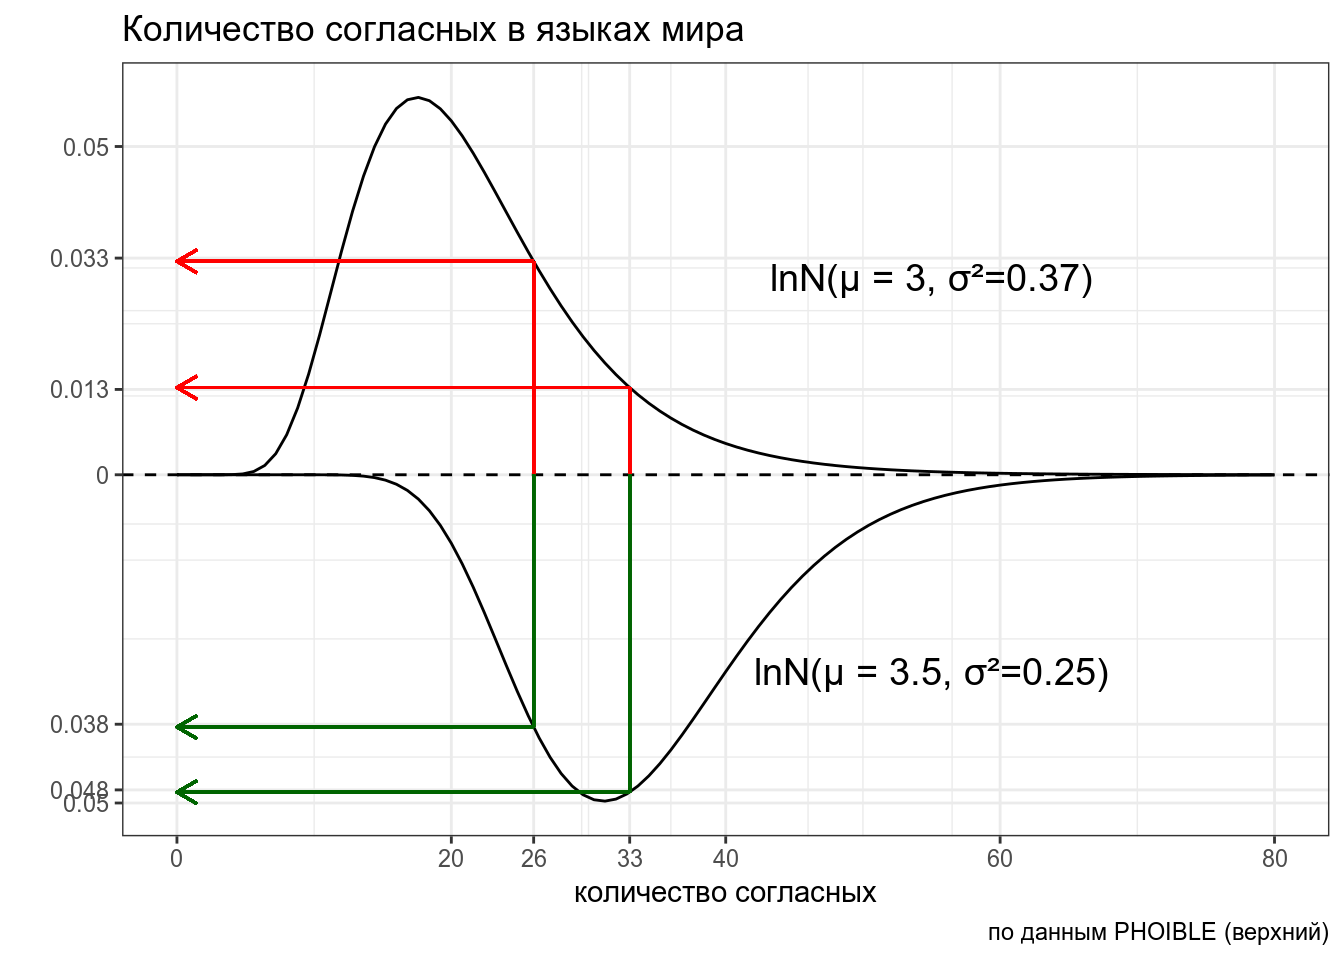
\includegraphics{da4l_files/figure-latex/unnamed-chunk-103-1.pdf}

\begin{Shaded}
\begin{Highlighting}[]
\NormalTok{L1 }\OtherTok{\textless{}{-}} \FunctionTok{dlnorm}\NormalTok{(}\DecValTok{33}\NormalTok{, }\DecValTok{3}\NormalTok{, }\FloatTok{0.37}\NormalTok{)}\SpecialCharTok{*}\FunctionTok{dlnorm}\NormalTok{(}\DecValTok{26}\NormalTok{, }\DecValTok{3}\NormalTok{, }\FloatTok{0.37}\NormalTok{)}
\NormalTok{L2 }\OtherTok{\textless{}{-}} \FunctionTok{dlnorm}\NormalTok{(}\DecValTok{33}\NormalTok{, }\FloatTok{3.5}\NormalTok{, }\FloatTok{0.25}\NormalTok{)}\SpecialCharTok{*}\FunctionTok{dlnorm}\NormalTok{(}\DecValTok{26}\NormalTok{, }\FloatTok{3.5}\NormalTok{, }\FloatTok{0.25}\NormalTok{)}
\NormalTok{L2}\SpecialCharTok{/}\NormalTok{L1}
\end{Highlighting}
\end{Shaded}

\begin{verbatim}
[1] 4.303835
\end{verbatim}

Как мы видим, на основании наших (фейковых) данных \(H_2\) в 4 раза более вероятнее, чем \(H_1\). Надо отметить, что не все тепло относятся к сравнению моделей (см. \href{https://citeseerx.ist.psu.edu/viewdoc/summary?doi=10.1.1.44.6443}{Gelman, Rubin 1994}).

\hypertarget{ux444ux43eux440ux43cux443ux43bux430-ux431ux430ux439ux435ux441ux430-ux43eux43fux44fux442ux44c}{%
\section{Формула Байеса опять}\label{ux444ux43eux440ux43cux443ux43bux430-ux431ux430ux439ux435ux441ux430-ux43eux43fux44fux442ux44c}}

Представим себе, что у нас есть \(k\) гипотез \(M\). Тогда формула Байеса может выглядеть вот так:

\[P(θ|Data, M_k) = \frac{P(Data|θ, M_k) \times  P(θ| M_k) }{P(Data|M_k)}\]

Коэффициент Байеса определяют как соотношение предельных правдоподобий (\(P(Data, M_k)\)) моделей (в принципе их может быть больше двух):

\[
BF_{12} = \frac{P(Data | M_1 )}{P(Data | M_2)}
\]

Вычислять предельные правдоподобия порой достаточно сложно, так что иногда используют численную аппроксимацию.

\hypertarget{ux431ux438ux43dux43eux43cux438ux430ux43bux44cux43dux44bux439-ux432ux430ux440ux438ux430ux43dux442}{%
\section{Биномиальный вариант}\label{ux431ux438ux43dux43eux43cux438ux430ux43bux44cux43dux44bux439-ux432ux430ux440ux438ux430ux43dux442}}

Рассмотрим пример эксперимента Бернулли:

\begin{itemize}
\tightlist
\item
  мы посчитали количество букв ``а'' в рассказе А. П. Чехова и получили 58 букв из рассказа длинной 699 букв (пробелы и латинские буквы выкинуты);
\item
  представим, что у нас есть две модели, соогласно одной мы ожидаем долю 0.08, а согласно другой 0.085.
\end{itemize}

Мы помним, что эксперимент Бернулли описывается биномиальным распределением:

\[P(k | n, p) = \frac{n!}{k!(n-k)!} \times p^k \times (1-p)^{n-k} =  {n \choose k} \times p^k \times (1-p)^{n-k}\]

Так что в случае наших моделей будет:

\[P(Data | M_1) = {n \choose k} \times p^k \times (1-p)^{n-k} = {699 \choose 58} \times 0.08^{58} \times (1-0.08)^{699-58} = 0.0523985\]

\begin{Shaded}
\begin{Highlighting}[]
\FunctionTok{dbinom}\NormalTok{(}\DecValTok{58}\NormalTok{, }\DecValTok{699}\NormalTok{, }\AttributeTok{prob =} \FloatTok{0.08}\NormalTok{)}
\end{Highlighting}
\end{Shaded}

\begin{verbatim}
[1] 0.0523985
\end{verbatim}

\[P(Data | M_2) = {n \choose k} \times p^k \times (1-p)^{n-k} = {699 \choose 58} \times 0.085^{58} \times (1-0.085)^{699-58} = 0.04402509\]

\begin{Shaded}
\begin{Highlighting}[]
\FunctionTok{dbinom}\NormalTok{(}\DecValTok{58}\NormalTok{, }\DecValTok{699}\NormalTok{, }\AttributeTok{prob =} \FloatTok{0.09}\NormalTok{)}
\end{Highlighting}
\end{Shaded}

\begin{verbatim}
[1] 0.04402509
\end{verbatim}

Тогда коэфициент Байеса будет

\begin{Shaded}
\begin{Highlighting}[]
\NormalTok{BF\_12 }\OtherTok{=} \FunctionTok{dbinom}\NormalTok{(}\DecValTok{58}\NormalTok{, }\DecValTok{699}\NormalTok{, }\AttributeTok{prob =} \FloatTok{0.08}\NormalTok{)}\SpecialCharTok{/}\FunctionTok{dbinom}\NormalTok{(}\DecValTok{58}\NormalTok{, }\DecValTok{699}\NormalTok{, }\AttributeTok{prob =} \FloatTok{0.09}\NormalTok{)}
\NormalTok{BF\_12}
\end{Highlighting}
\end{Shaded}

\begin{verbatim}
[1] 1.190196
\end{verbatim}

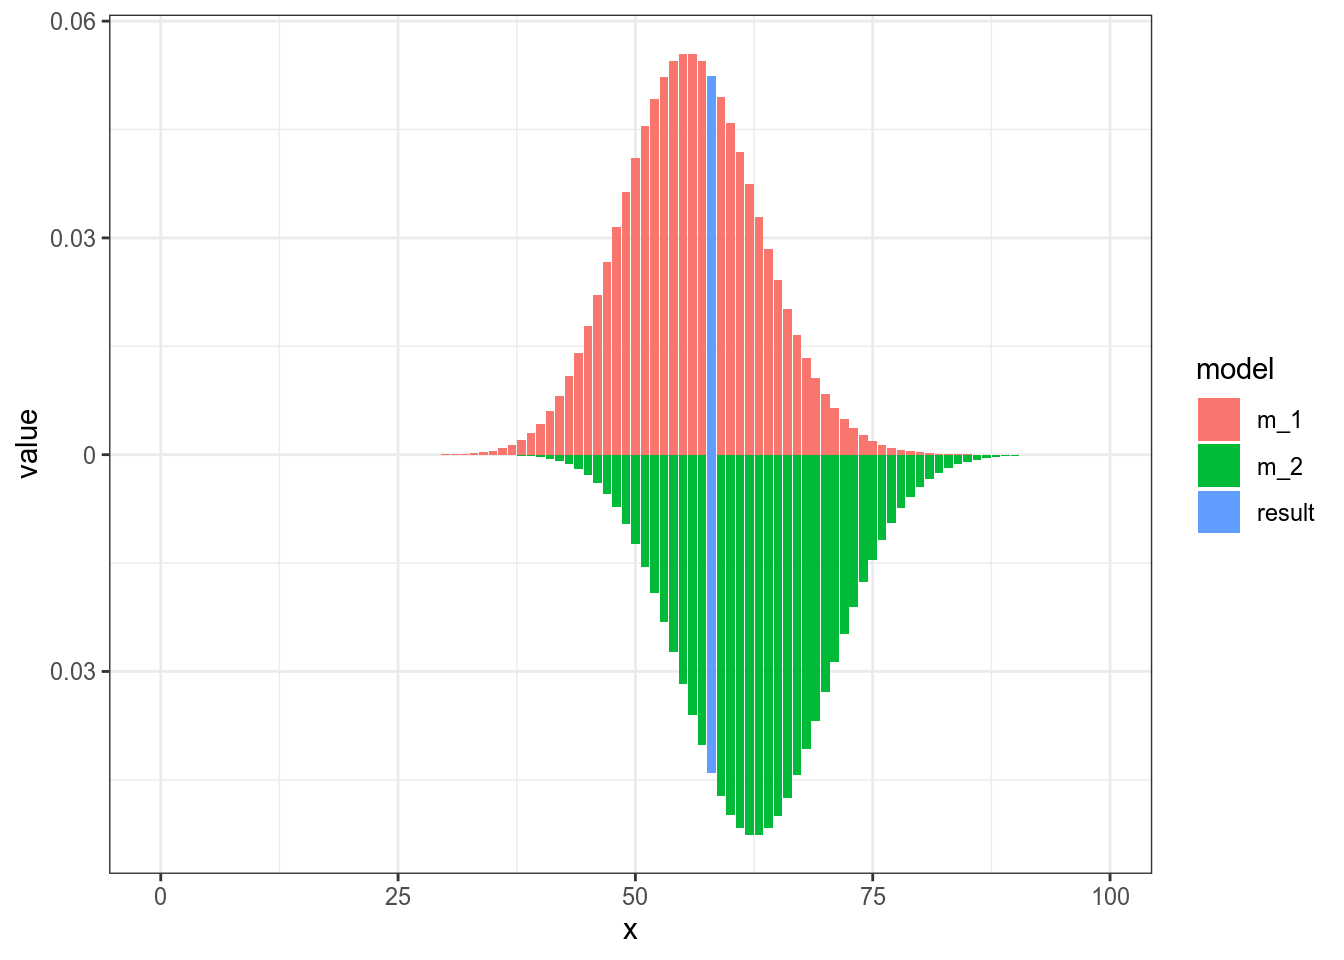
\includegraphics{da4l_files/figure-latex/unnamed-chunk-108-1.pdf}

\hypertarget{ux438ux43dux442ux435ux440ux43fux440ux435ux442ux430ux446ux438ux44f-ux43aux43eux44dux444ux444ux438ux446ux438ux435ux43dux442ux430-ux431ux430ux439ux435ux441ux430}{%
\section{\texorpdfstring{\href{https://en.wikipedia.org/wiki/Bayes_factor\#Interpretation}{Интерпретация коэффициента Байеса}}{Интерпретация коэффициента Байеса}}\label{ux438ux43dux442ux435ux440ux43fux440ux435ux442ux430ux446ux438ux44f-ux43aux43eux44dux444ux444ux438ux446ux438ux435ux43dux442ux430-ux431ux430ux439ux435ux441ux430}}

\hypertarget{ux434ux438ux441ux43aux440ux435ux442ux43dux44bux439-ux432ux430ux440ux438ux430ux43dux442}{%
\section{Дискретный вариант}\label{ux434ux438ux441ux43aux440ux435ux442ux43dux44bux439-ux432ux430ux440ux438ux430ux43dux442}}

Для примера обратися снова к датасету, который содержит спамерские и обычные смс-сообщения, выложенный UCI Machine Learning \href{https://www.kaggle.com/uciml/sms-spam-collection-dataset}{на kaggle} и при помощи пакета \texttt{udpipe} токенизировал и определил часть речи:

\begin{Shaded}
\begin{Highlighting}[]
\NormalTok{sms\_pos }\OtherTok{\textless{}{-}} \FunctionTok{read\_csv}\NormalTok{(}\StringTok{"https://raw.githubusercontent.com/agricolamz/2021\_da4l/master/data/spam\_sms\_pos.csv"}\NormalTok{)}
\FunctionTok{glimpse}\NormalTok{(sms\_pos)}
\end{Highlighting}
\end{Shaded}

\begin{verbatim}
Rows: 34
Columns: 3
$ type <chr> "ham", "ham", "ham", "ham", "ham", "ham", "ham", "ham", "ham",...
$ upos <chr> "ADJ", "ADP", "ADV", "AUX", "CCONJ", "DET", "INTJ", "NOUN", "N...
$ n    <dbl> 4329, 5004, 5832, 5707, 1607, 3493, 1676, 12842, 1293, 2424, 1...
\end{verbatim}

\begin{Shaded}
\begin{Highlighting}[]
\NormalTok{sms\_pos }\SpecialCharTok{\%\textgreater{}\%} 
  \FunctionTok{group\_by}\NormalTok{(type) }\SpecialCharTok{\%\textgreater{}\%} 
  \FunctionTok{mutate}\NormalTok{(}\AttributeTok{ratio =}\NormalTok{ n}\SpecialCharTok{/}\FunctionTok{sum}\NormalTok{(n),}
         \AttributeTok{upos =} \FunctionTok{fct\_reorder}\NormalTok{(upos, n, mean, }\AttributeTok{.desc =} \ConstantTok{TRUE}\NormalTok{)) }\SpecialCharTok{\%\textgreater{}\%}
  \FunctionTok{ggplot}\NormalTok{(}\FunctionTok{aes}\NormalTok{(type, ratio))}\SpecialCharTok{+}
  \FunctionTok{geom\_col}\NormalTok{()}\SpecialCharTok{+}
  \FunctionTok{geom\_label}\NormalTok{(}\FunctionTok{aes}\NormalTok{(}\AttributeTok{label =} \FunctionTok{round}\NormalTok{(ratio, }\DecValTok{3}\NormalTok{)), }\AttributeTok{position =} \FunctionTok{position\_stack}\NormalTok{(}\AttributeTok{vjust =} \FloatTok{0.5}\NormalTok{))}\SpecialCharTok{+}
  \FunctionTok{facet\_wrap}\NormalTok{(}\SpecialCharTok{\textasciitilde{}}\NormalTok{upos, }\AttributeTok{scales =} \StringTok{"free\_y"}\NormalTok{)}
\end{Highlighting}
\end{Shaded}

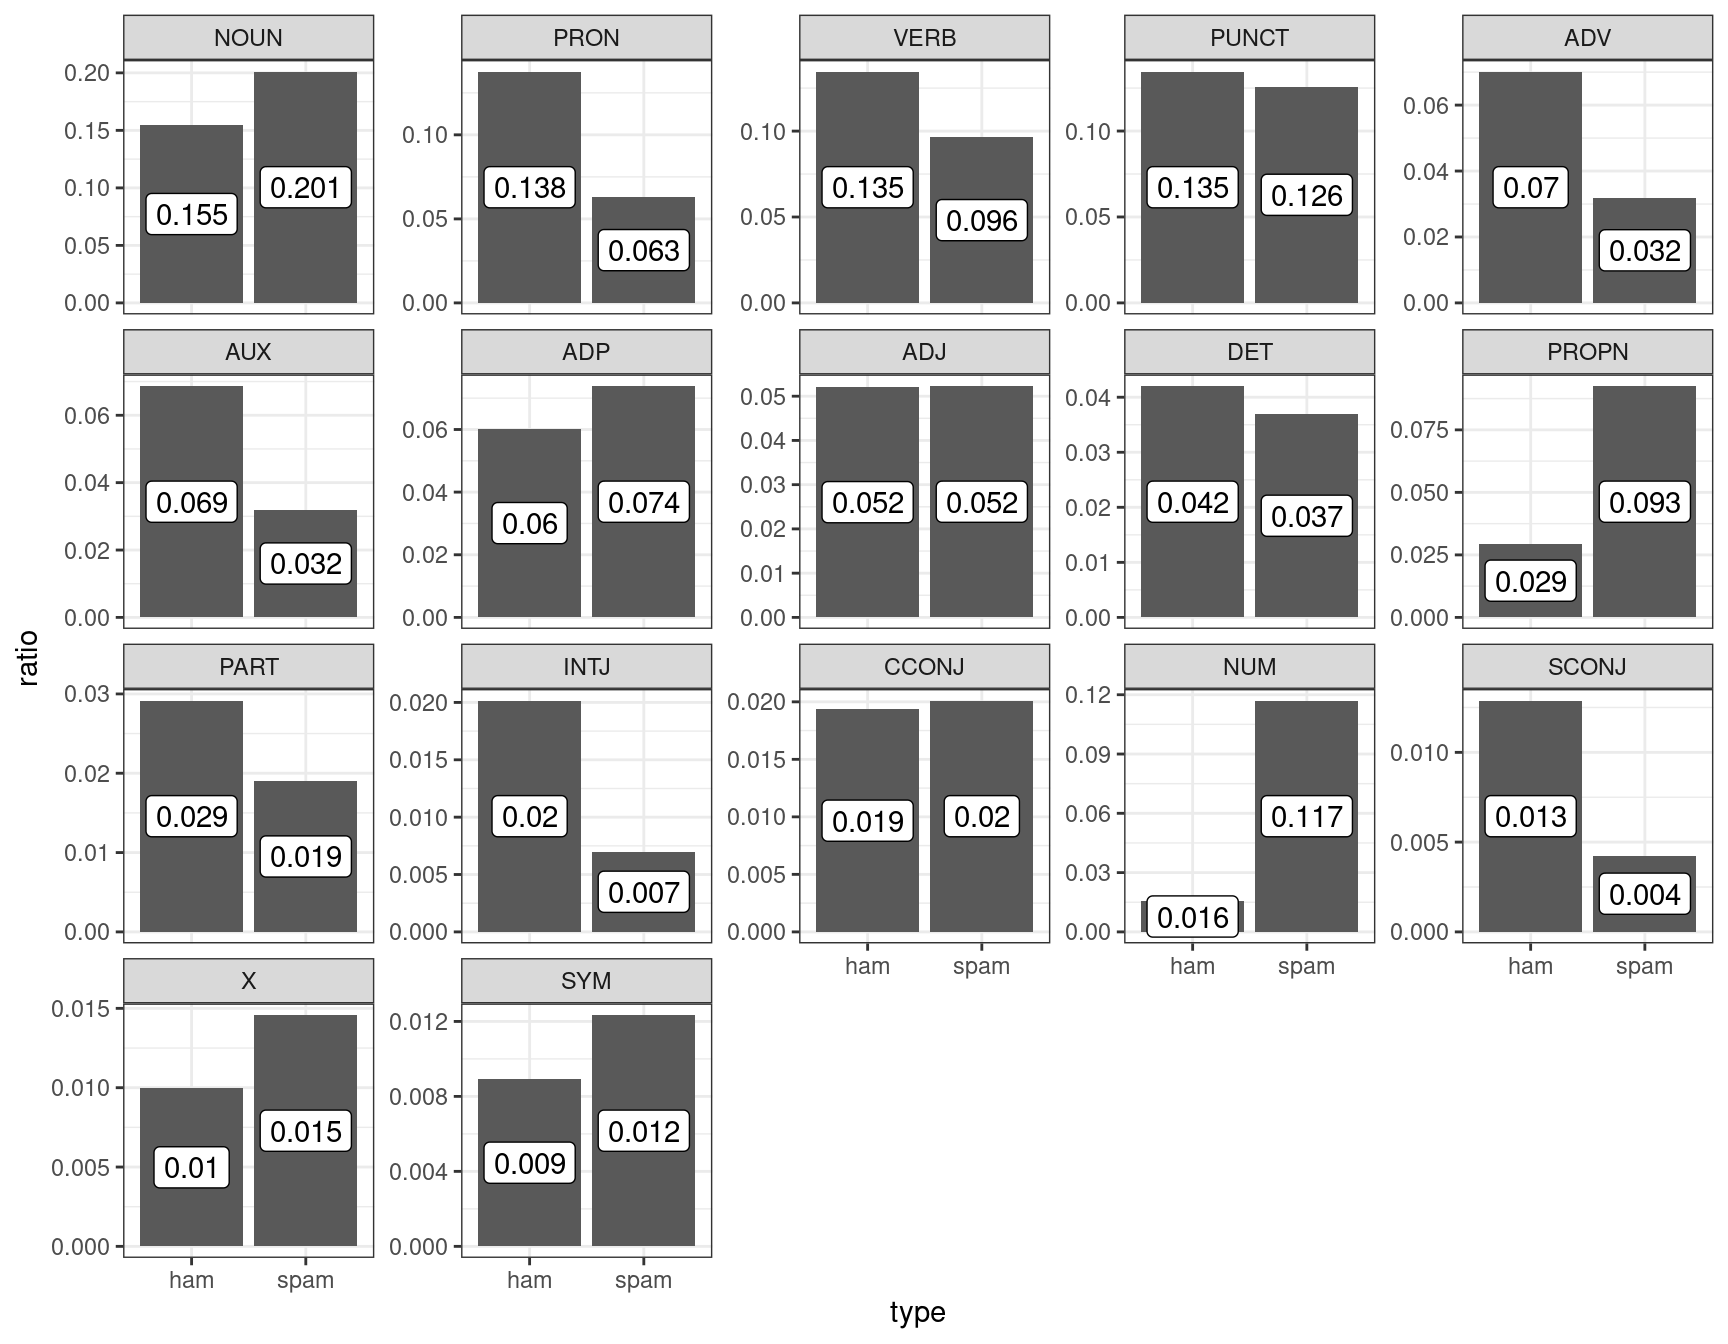
\includegraphics{da4l_files/figure-latex/unnamed-chunk-109-1.pdf}

Давайте полученные доли считать нашей моделью: сумма всех чисел внутри каждого типа (\texttt{ham}/\texttt{spam}) дает в сумме 1. Мы получили новое сообщение:

\begin{quote}
Call FREEPHONE 0800 542 0825 now!
\end{quote}

Модель \texttt{udpipe} разобрала его следующим образом:

\begin{quote}
VERB NUM NUM NUM NUM ADV PUNCT
\end{quote}

\[L(VERB,\ NUM|ham) = 0.135 \times 0.016 = 0.00216\]

\[L(VERB,\ NUM|spam) = 0.096 \times 0.117 = 0.011232\]

\[BF_{ham\ spam} = \frac{L(VERB,\ NUM|ham)}{L(VERB,\ NUM|spam)} = \frac{0.00216}{0.011232} = 0.1923077\]

\hypertarget{ux43dux435ux441ux43aux43eux43bux44cux43aux43e-ux442ux43eux447ux435ux447ux43dux44bux445-ux43cux43eux434ux435ux43bux435ux439}{%
\section{Несколько точечных моделей}\label{ux43dux435ux441ux43aux43eux43bux44cux43aux43e-ux442ux43eux447ux435ux447ux43dux44bux445-ux43cux43eux434ux435ux43bux435ux439}}

До сих пор мы рассматривали одну точечную модель, сравнивая доли 0.08 и 0.085.

\begin{itemize}
\tightlist
\item
  Мы посчитали количество букв ``а'' в рассказе А. П. Чехова и получили 58 букв из рассказа длинной 699 букв (пробелы и латинские буквы выкинуты);
\item
  представим, что у нас есть две модели, соогласно одной мы ожидаем долю 0.08, а вторая модель состоит из 7 равновероятных моделей: 0.60 0.65 0.70 0.75 0.80 0.85 0.90.
\end{itemize}

Функцию правдоподобия для первой модели мы уже считали:

\begin{Shaded}
\begin{Highlighting}[]
\FunctionTok{dbinom}\NormalTok{(}\DecValTok{58}\NormalTok{, }\DecValTok{699}\NormalTok{, }\AttributeTok{prob =} \FloatTok{0.08}\NormalTok{)}
\end{Highlighting}
\end{Shaded}

\begin{verbatim}
[1] 0.0523985
\end{verbatim}

Функция правдоподобия второй модели -- это среднее функций правдоподобия всех входящих моделей:

\begin{Shaded}
\begin{Highlighting}[]
\FunctionTok{mean}\NormalTok{(}\FunctionTok{dbinom}\NormalTok{(}\DecValTok{58}\NormalTok{, }\DecValTok{699}\NormalTok{, }\AttributeTok{prob =} \FunctionTok{seq}\NormalTok{(}\FloatTok{0.08}\NormalTok{, }\FloatTok{0.085}\NormalTok{, }\FloatTok{0.001}\NormalTok{)))}
\end{Highlighting}
\end{Shaded}

\begin{verbatim}
[1] 0.05383749
\end{verbatim}

Байес фактор:

\begin{Shaded}
\begin{Highlighting}[]
\FunctionTok{mean}\NormalTok{(}\FunctionTok{dbinom}\NormalTok{(}\DecValTok{58}\NormalTok{, }\DecValTok{699}\NormalTok{, }\AttributeTok{prob =} \FunctionTok{seq}\NormalTok{(}\FloatTok{0.08}\NormalTok{, }\FloatTok{0.085}\NormalTok{, }\FloatTok{0.001}\NormalTok{)))}\SpecialCharTok{/}\FunctionTok{dbinom}\NormalTok{(}\DecValTok{58}\NormalTok{, }\DecValTok{699}\NormalTok{, }\AttributeTok{prob =} \FloatTok{0.08}\NormalTok{)}
\end{Highlighting}
\end{Shaded}

\begin{verbatim}
[1] 1.027462
\end{verbatim}

Как видим, наша распределенная модель немного предпочтительнее, чем точечная.

  \bibliography{bibliography.bib}

\end{document}
